\documentclass{scrartcl}
\usepackage{style}

% version
\newcommand{\versionmajor}{2}
\newcommand{\versionminor}{0}
\newcommand{\versionpatch}{0}
\newcommand{\version}{\versionmajor.\versionminor.\versionpatch}

\title{\LARGE
    ChainVote Final Report
}

\subtitle{(v. \version)}

\author{
    Giovanni Antonioni \\ \emailaddr{giovanni.antonioni2@studio.unibo.it} \\ Matr. \texttt{xxxx}
    \and 
    Luca Rubboli \\ \emailaddr{luca.rubboli2@studio.unibo.it} \\ Matr. \texttt{1083742}
    \and
    Luca Tassinari \\ \emailaddr{luca.tassinari10@studio.unibo.it} \\ Matr. \texttt{1096190}
}

\date{\today}

\begin{document}

\maketitle

\begin{abstract}
    Electronic voting systems based on blockchain technology have emerged as a potential solution to enhance the security and transparency of traditional voting methods. In this system, voters cast their votes electronically, and the results are stored on a decentralized blockchain ledger, which ensures the integrity of the vote by preventing any tampering or manipulation. This system provides a transparent and immutable record of votes, which can be accessed by anyone in the network, thus increasing trust in the electoral process. Nevertheless, the use of blockchain technology in electronic voting systems holds promise for creating a more secure, transparent, and democratic electoral process.
\end{abstract}

\section{Goals and requirements}

The project consists of the implementation of a small-scale distributed electronic voting system based on blockchain technology.
%
Specifically, the goal is to create a \textbf{distributed architecture} that exposes a \textbf{uniform API} allowing users to interact with the system using a \textbf{web application}.

\subsection{Functional requirements}

Here are reported the set of questions and answers used to refine the coarse-grained system's requirements.

\begin{Question}
    What are the main actors of the system?
\end{Question}
\begin{Answer}
    Two main actors can be identified in the system: the \textbf{administrator}, taking care of creating new elections, and the \textbf{user}, which interacts with them.
\end{Answer}

\begin{Question}
    Can everybody create a new election?
\end{Question}
\begin{Answer}
    No, only system administrators can create new elections.
\end{Answer}

\begin{Question}
    Can everybody cast votes?
\end{Question}
\begin{Answer}
    System administrators can't cast a vote, while regular users are allowed to cast a vote only once authenticated.
\end{Answer}

\begin{Question}
    How many times can a user cast votes in a single election?
\end{Question}
\begin{Answer}
    A user can cast a vote up to once per ballot.
\end{Answer}

\begin{Question}
    What is an election?
\end{Question}
\begin{Answer}
    An election is a set of mutually exclusive choices with a time limit that cannot be changed.
\end{Answer}

\begin{Question}
    Can a user modify their vote?
\end{Question}
\begin{Answer}
    No, once a vote has been cast it cannot be modified.
\end{Answer}

\begin{Question}
    Which information about the election is available to users?
\end{Question}
\begin{Answer}
    While a vote is open users can see only the turnout. Once an election is closed, all users (voters and abstainers) and administrators can see the results. At the application level, the connection between a user and his vote must be hidden.
\end{Answer}

\begin{Question}
    Is it possible to have multiple elections open at the same time?
\end{Question}
\begin{Answer}
    Yes.
\end{Answer}

\begin{Question}
    Users get some kind of notifications?
\end{Question}
\begin{Answer}
    Users are notified whenever a new election opens and is about to close.
\end{Answer}

The above user requirements have emphasized the use cases reported in \Cref{fig:use-cases-diagram}.

\begin{figure}
    \centering
    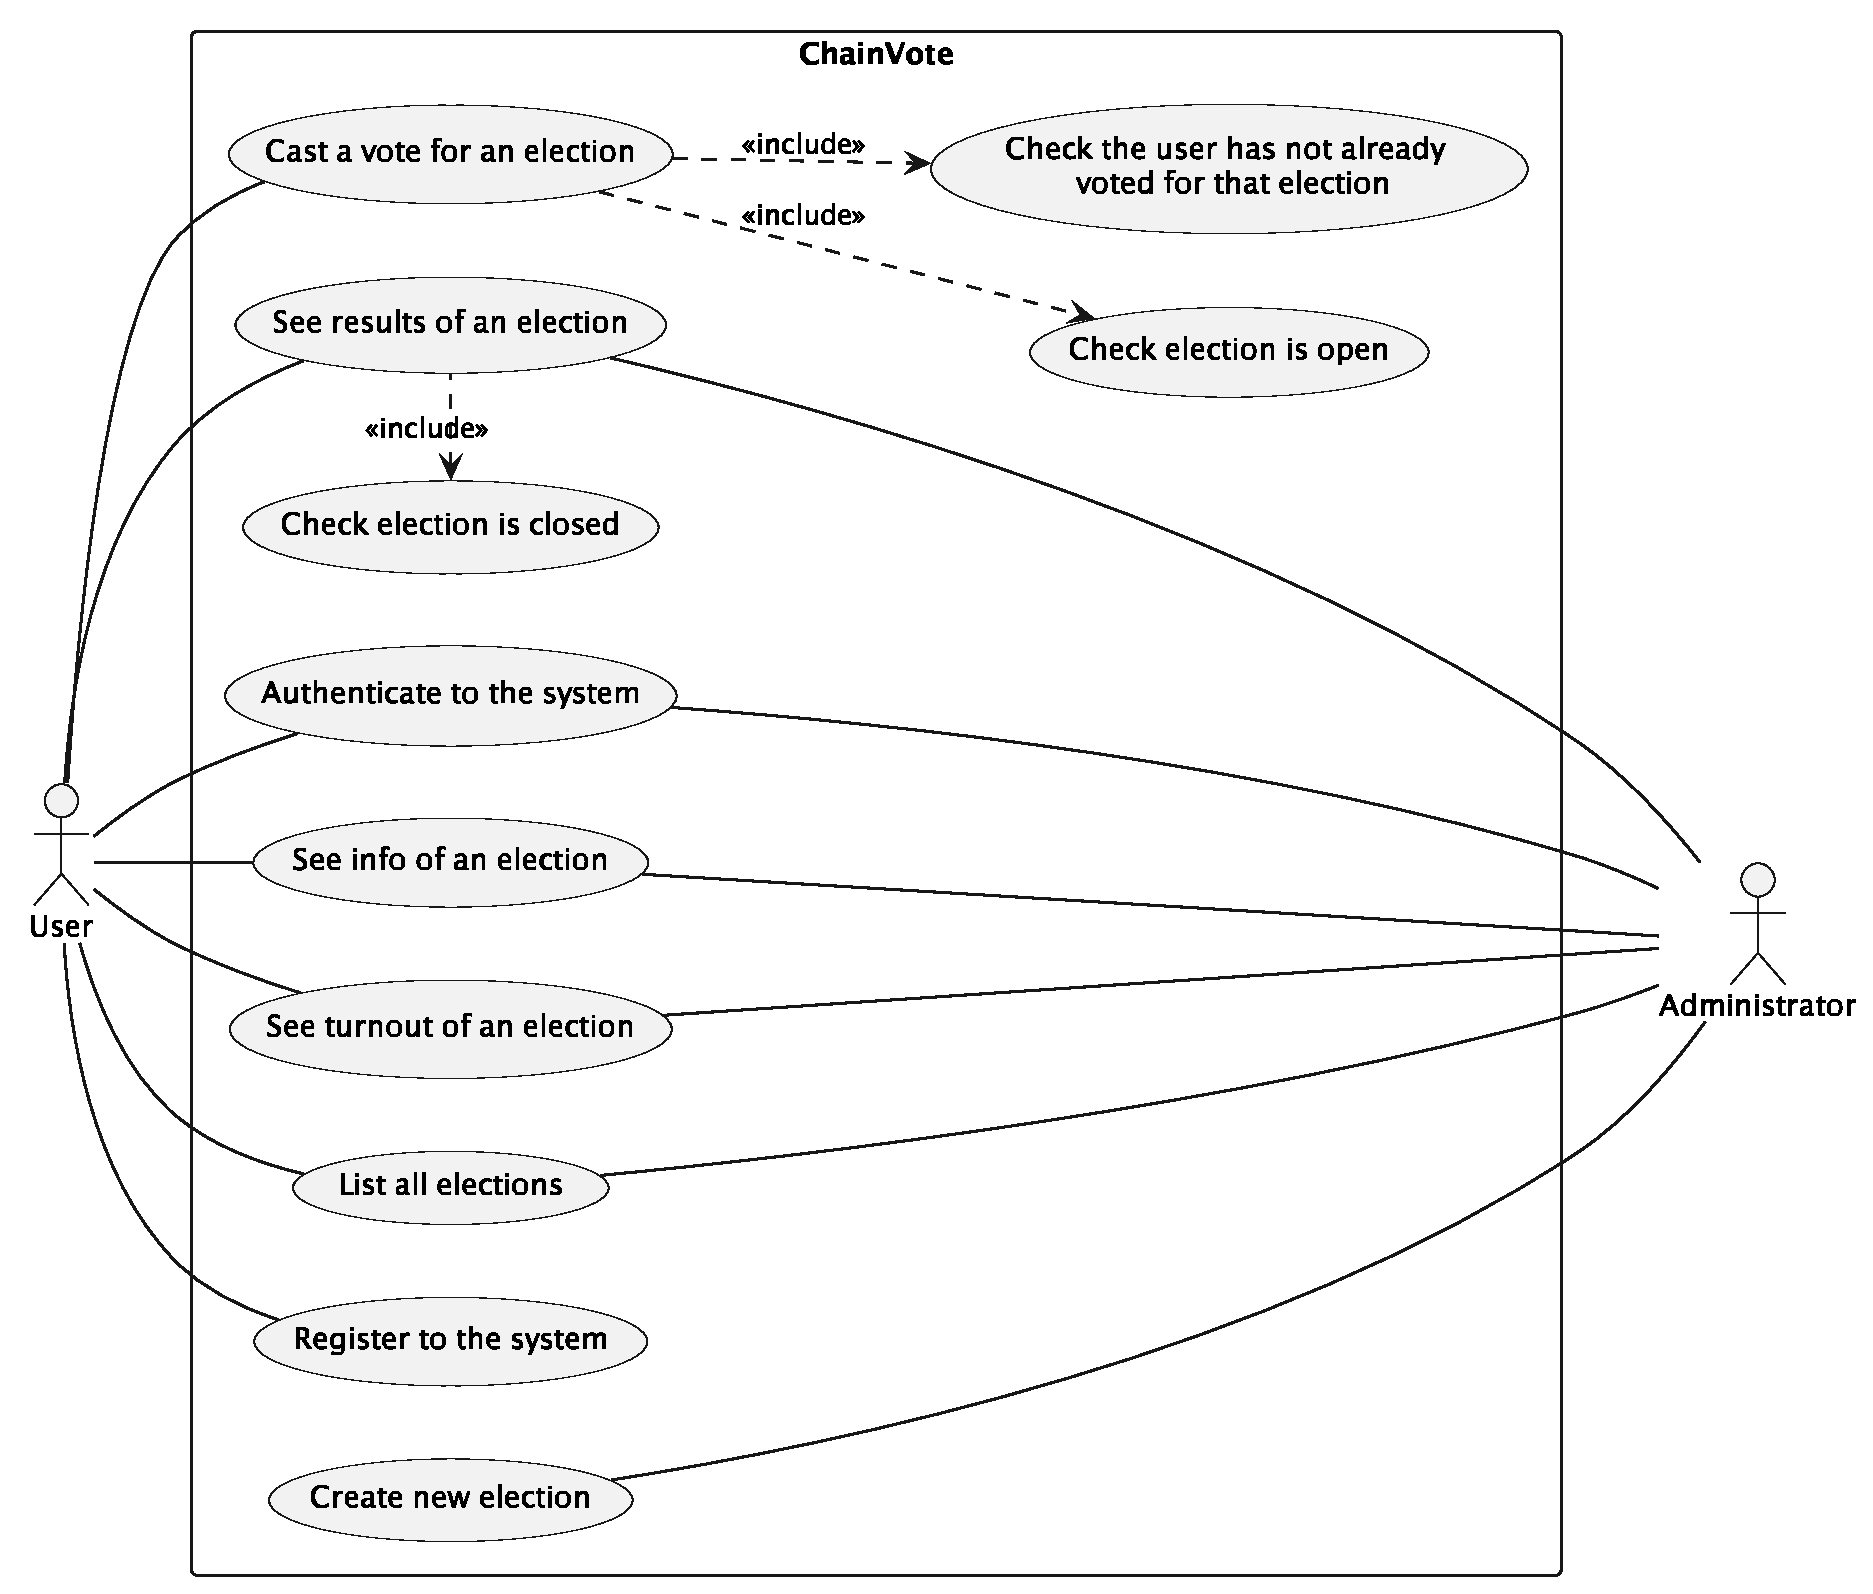
\includegraphics[width=\linewidth]{figures/use-cases.eps}
    \caption{Use cases diagram of the ChainVote application.}
    \label{fig:use-cases-diagram} 
\end{figure}

\subsection{Non functional requirements}
\label{sec:non-functional-requirements}

In order to decouple as much as possible users from their vote inside the blockchain and make it more difficult for unauthorized individuals to cast a vote impersonating someone else, \textbf{pseudo-random one-time codes} will be used.
%
The idea is that, before casting a new vote, the user requests a one-time code that is sent to him using a different trusted method.
%
When voting, the user will have to send back the generated one-time code to the system to correctly submit his vote.
%
The outline of use cases related to the casting of a vote in light of the above refinements is presented in \Cref{fig:refined-cast-vote-use-case}.

\begin{figure}
    \centering
    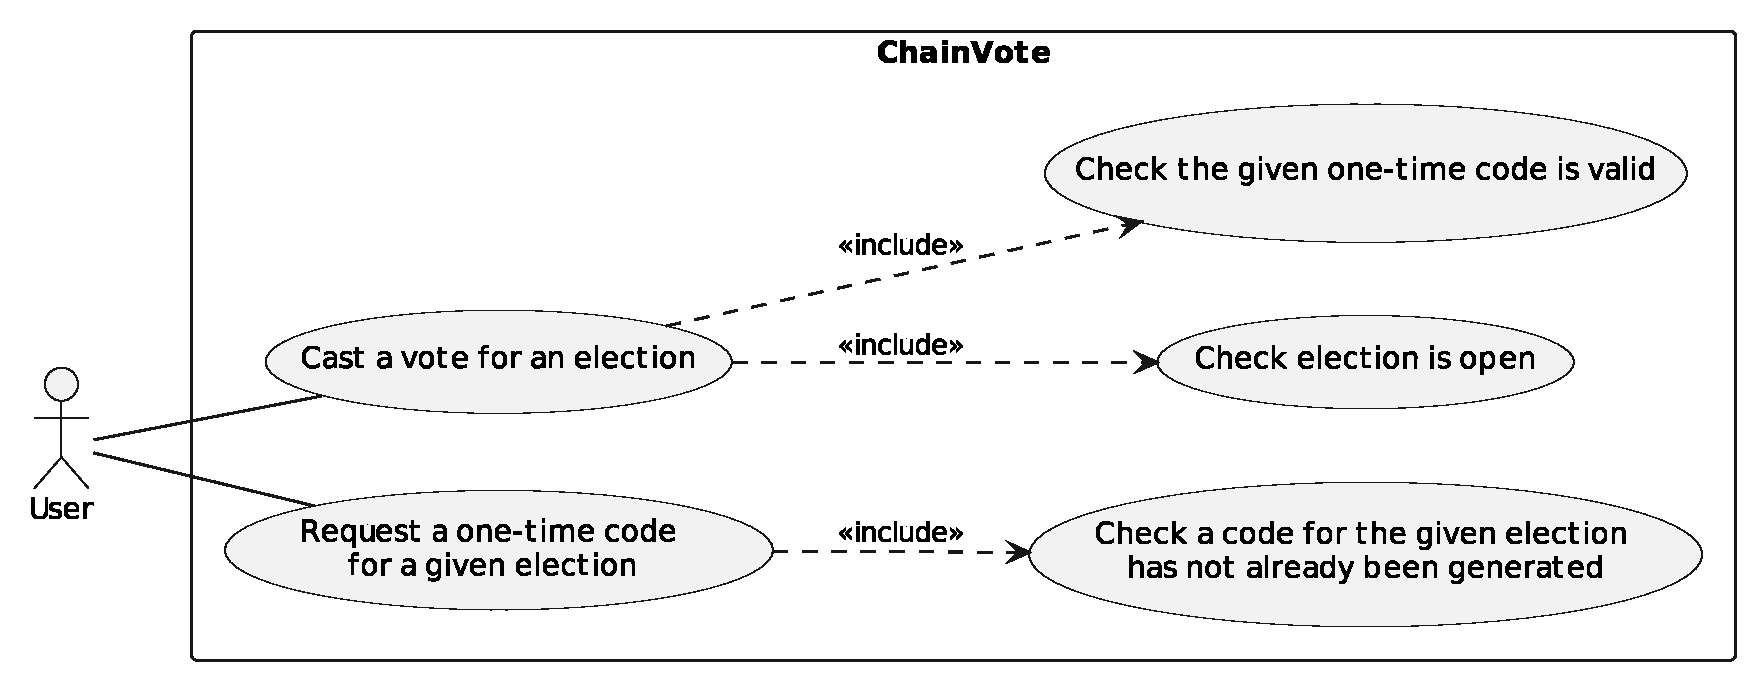
\includegraphics[width=\linewidth]{figures/refined-cast-vote-use-case.eps}
    \caption{Refined use case diagram for the casting of a vote.}
    \label{fig:refined-cast-vote-use-case}
\end{figure}

%% -------------------------------------- DS ----------------------------
\iffalse

To accomplish this, two challenges must be faced during the design process:

\begin{itemize}
    \item It is necessary that, within the ledger, the code-user association, as well as the expressed vote and user's code, are stored securely, i.e. are not recorded in clear in the blockchain bocks' transactions;
    \item Given that the deterministic nature of smart contracts makes it difficult to generate completely random codes, a deterministic algorithm will be used and a source of randomness will be injected from a trusted and controlled entity. It's worth mentioning their generation \textit{a priori} (i.e. when the election is created) is not feasible since smart contract transactions are executed by peers in any order, possibly even in parallel, implying that different peers may process the same client transaction with different order. This means that it is not possible to guarantee that, when the client triggers the transaction execution, peers will get the same code from the set of already generated ones.
\end{itemize}

\fi
%% -------------------------------------- DS ----------------------------

Moreover, for security reasons, the \textbf{user's password should not be stored in plain text} within the server storage, but password encryption mechanisms will have to be employed.

The web application must be designed to be accessible and have a user experience that allows even less experienced users to use it easily. For this, the design must be designed to be \textbf{responsive} and \textbf{mobile-first}. In addition, an important feature that must be supported is the responsiveness of the interface, which must be able to refresh and show voting-related information in \textbf{real-time} without having to refresh the page.

\subsection{Target User Analysis}

In order to meet the non functional properties concerning the user experience it's important to have a comprehensive understanding of our target audience.
%
In the next section is presented the target user analysis that serves as the compass guiding our decisions.

\subsubsection*{Admin users}

\noindent
\emph{%
    As an administrator (who), \\ 
    I want to create an election (what), \\ 
    So that interested users can express their vote (why).
}
\vspace*{0.2cm}

\textbf{Personas:} Alba

Alba is an administrator of the ChainVote system.

\textbf{Use Case Scenario:}

The University of Bologna needs to elect the next rector and wants to collect votes through the ChainVote system. Alba is tasked with creating the election.

\begin{enumerate}
    \item Alba logs into the platform using her credentials;
    \item Alba navigates to the "Create Election" section;
    \item Alba enters the election details:
    \begin{itemize}
        \item Estimated number of voters;
        \item Election start date;
        \item Election end date;
        \item Goal (election title);
        \item Choices.
    \end{itemize}
    \item Alba saves the election.
\end{enumerate}

\vspace*{0.5cm}
\noindent
\emph{%
    As an administrator (who), \\
    I want to view the election results (what), \\
    To make a decision regarding the consequences of the election (why).
}
\vspace*{0.2cm}

\textbf{Personas:} Giovanni

Giovanni is the rector of the University of Bologna.

\textbf{Use Case Scenario:}

Giovanni wants to view the results of the vote concerning the next rector of the University of Bologna so that he can congrats to him.

\begin{enumerate}
    \item Giovanni accesses the system with his credentials;
    \item Giovanni navigates to the "Dashboard" page;
    \item Giovanni selects the election with the goal "Next rector of UniBo";
    \item Giovanni verifies that the vote is closed;
    \item Giovanni views the results related to the election and the turnout.
\end{enumerate}

\subsubsection*{Users}

\noindent
\emph{%
    As a user (who), \\
    I want to access the system (what), \\
    To be able to use various functionalities (why).
}
\vspace*{0.2cm}

\textbf{Personas:} Luca

Luca is a university student in Engineering and Computer Science at the University of Bologna, Cesena campus.

\textbf{Use Case Scenario:}

Luca wants to connect to the system to view upcoming elections.

\begin{enumerate}
    \item Luca goes to the login page;
    \item Luca enters his username and password in the respective fields;
    \item Luca clicks the login button;
    \item Luca gets redirected to the Dashboard where all the elections are displayed.
\end{enumerate}

\vspace*{0.5cm}
\noindent
\emph{%
    As a user (who), \\
    I want to view system notifications (what), \\
    To stay updated (why).
}
\vspace*{0.2cm}

\textbf{Personas:} Deborah

Deborah is an out-of-town student. 

\textbf{Use Case Scenario:}

Deborah is waiting for the opening of the election and wants to receive and see a notification as soon as an election opens or is about to close.

\begin{enumerate}
    \item Deborah logs into the system with his credentials;
    \item Deborah views if there are new notifications from the navbar icon that signals not read notification;
    \item Deborah clicks on the navbar link that takes to the page related to her notifications;
    \item Deborah is notified by a toast popup if a notification is triggered by the server.
\end{enumerate}

\vspace*{0.5cm}
\noindent
\emph{%
    As a user (who), \\
    I want to request a one time code for an election (what), \\
    so that I can cast a vote for it (why).
}
\vspace*{0.2cm}

\textbf{Personas:} Oscar

Oscar is a member of the UniBo Council. 

\textbf{Use Case Scenario:}

Oscar wants to request a code to participate in the vote regarding the next rector of UniBo.

\begin{enumerate}
    \item Oscar logs into the system with his credentials;
    \item Oscar navigates to the "Dashboard";
    \item Oscar verifies that the election is open;
    \item Oscar accesses the code request area;
    \item Oscar clicks the button to request the code;
    \item Oscar views part of the code internally in a form on the page, and the other half is sent to his email address.
\end{enumerate}

\vspace*{0.2cm}
\noindent
\emph{%
    As a user (who), \\
    I want to cast a vote in an election (what), \\
    To express my preference (why).
}
\vspace*{0.2cm}

\textbf{Use Case Scenario:}

Oscar, after obtaining the code, wants to cast his vote.

\begin{enumerate}
    \item Oscar logs into the system with his credentials;
    \item Oscar navigates to the "Dashboard";
    \item Oscar verifies that the election is open;
    \item Oscar accesses the vote area;
    \item Oscar enters the code for the vote (previously obtained);
    \item Oscar chooses an option.
\end{enumerate}

\vspace*{0.2cm}
\noindent
\emph{%
    As a user (who), \\
    I want to view the results of an election (what),
    To understand the preferences expressed by users regarding the election (why).
}
\vspace*{0.2cm}

\textbf{Use Case Scenario:}

Oscar wants to view the results of the election.

\begin{enumerate}
    \item Oscar logs into the system with his credentials;
    \item Oscar navigates to the Dashboard;
    \item Oscar selects the election of his interest;
    \item Oscar verifies that the vote is closed;
    \item Oscar views the results related to the vote.
\end{enumerate}

\vspace*{0.5cm}
\noindent
\emph{%
    As a user (who), \\
    I want to change my password (what), \\
    So that I can access the system again (why).
}
\vspace*{0.2cm}

\textbf{Personas:} Aurora

Aurora is a kindly elderly person. 

\textbf{Use Case Scenario:}

Aurora wants to access the system after a long period and realizes she has forgotten the login password for her account.

\begin{enumerate}
    \item Aurora connects to the login page;
    \item Aurora clicks the "recover password" link;
    \item Aurora enters her information (email) and clicks the "Recover Password" button;
    \item Aurora receives instructions to reset the password at the email address provided in the previous step;
    \item Aurora logins again into the system.
\end{enumerate}

\section{Design}

This section present the overall design of the system, both frontend and backend side.

\subsection{Frontend design}

\subsubsection*{Mockups}

Style in a web application is an important aspect to consider to fulfill usability requirements described above.
%
In order to devise a design that would enable a good user experience of the final product, initial mockups had to be carried out. 

As already specified in the non-functional requirements, design of the application is mobile-first. 
%
This means that mockups have been made and thought out in their elements primarily in the mobile context and adapted to be usable in a user-friendly manner and taking advantage of all the spaces available in the desktop version.

The only page accessible by unauthenticated users is the home page where is described the purpose of the project.

The user, in order to use the system, is required to log in (\Cref{fig:login-dashboard-elections-views}).
%
Once correctly logged, the user is redirected to the Dashboard where all the elections are displayed, categorized by "Open", "Closed" and "Soon".

Reasoning about usability, has been decided to add another view, Election view, where elections can be displayed, rather categorized or unfiltered. Moreover, vertical display allows a smoother visualization, up to 10 per page even in mobile setting.
%
From both visualization views, users can see the details of an election (\Cref{fig:details-cast-notifications-view}), ask for the code required during voting phase as well as reach the page to cast a new vote.
%
From the navbar is possible to navigate the notifications view where all recent notifications are displayed along with an indication of whether it has already been read or not.

\begin{figure}[h]
    \centering
    \begin{subfigure}[b]{0.3\textwidth}
        \centering
        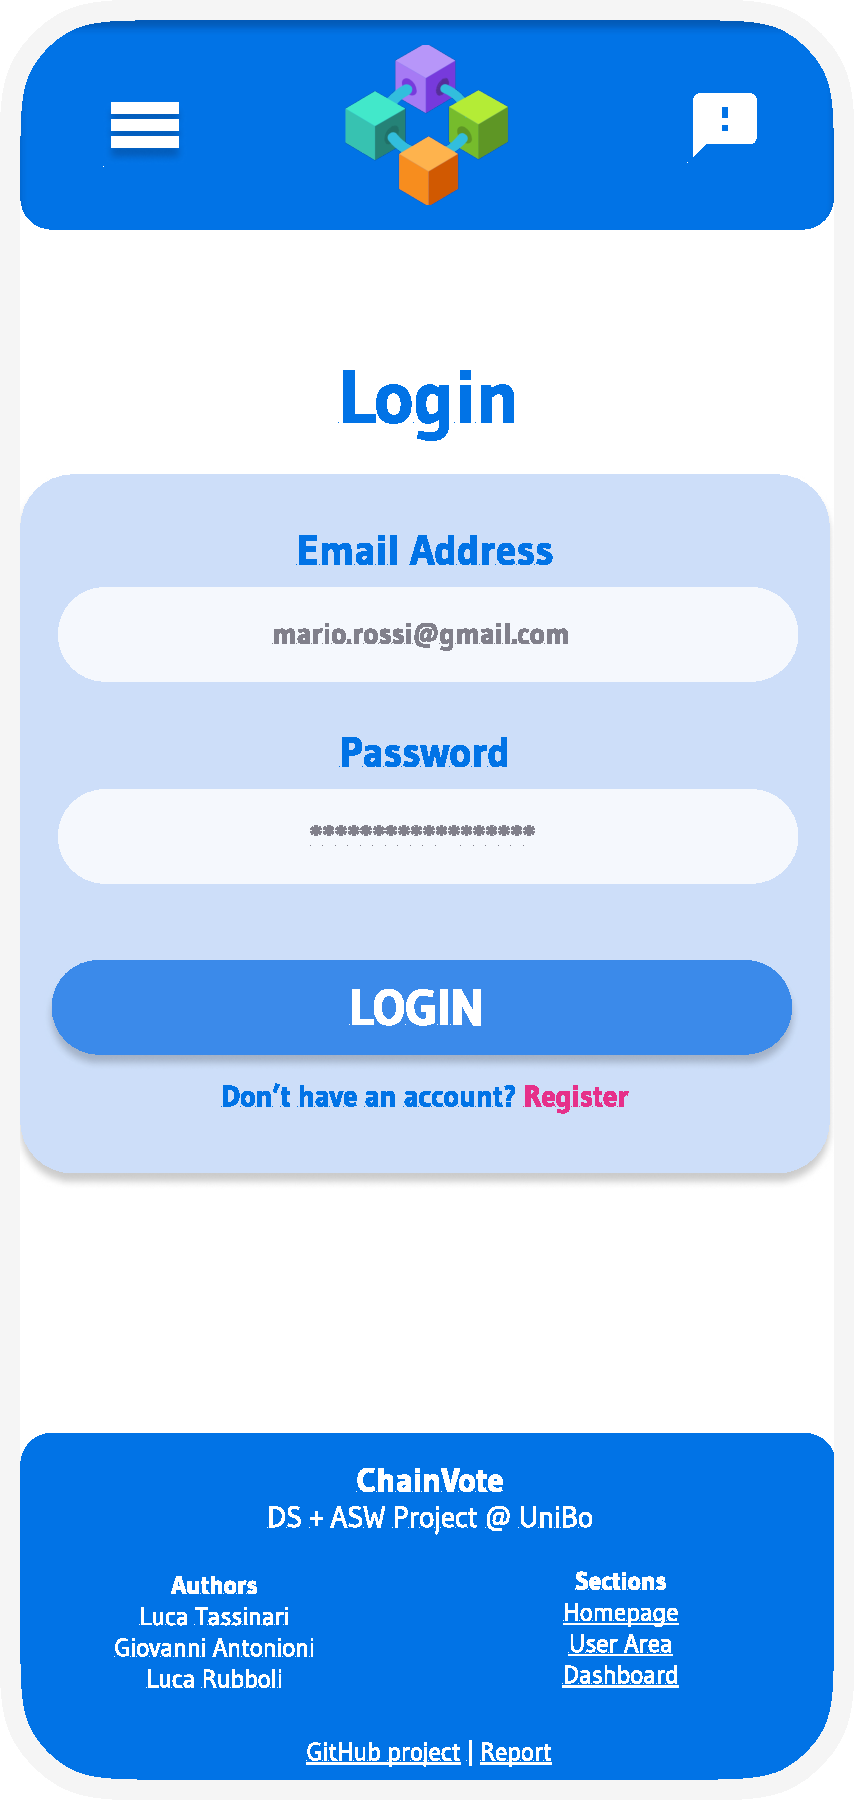
\includegraphics[width=\textwidth]{./figures/mockups/login.pdf}
        %\caption{}
    \end{subfigure}
    \hfill
    \begin{subfigure}[b]{0.3\textwidth}
        \centering
        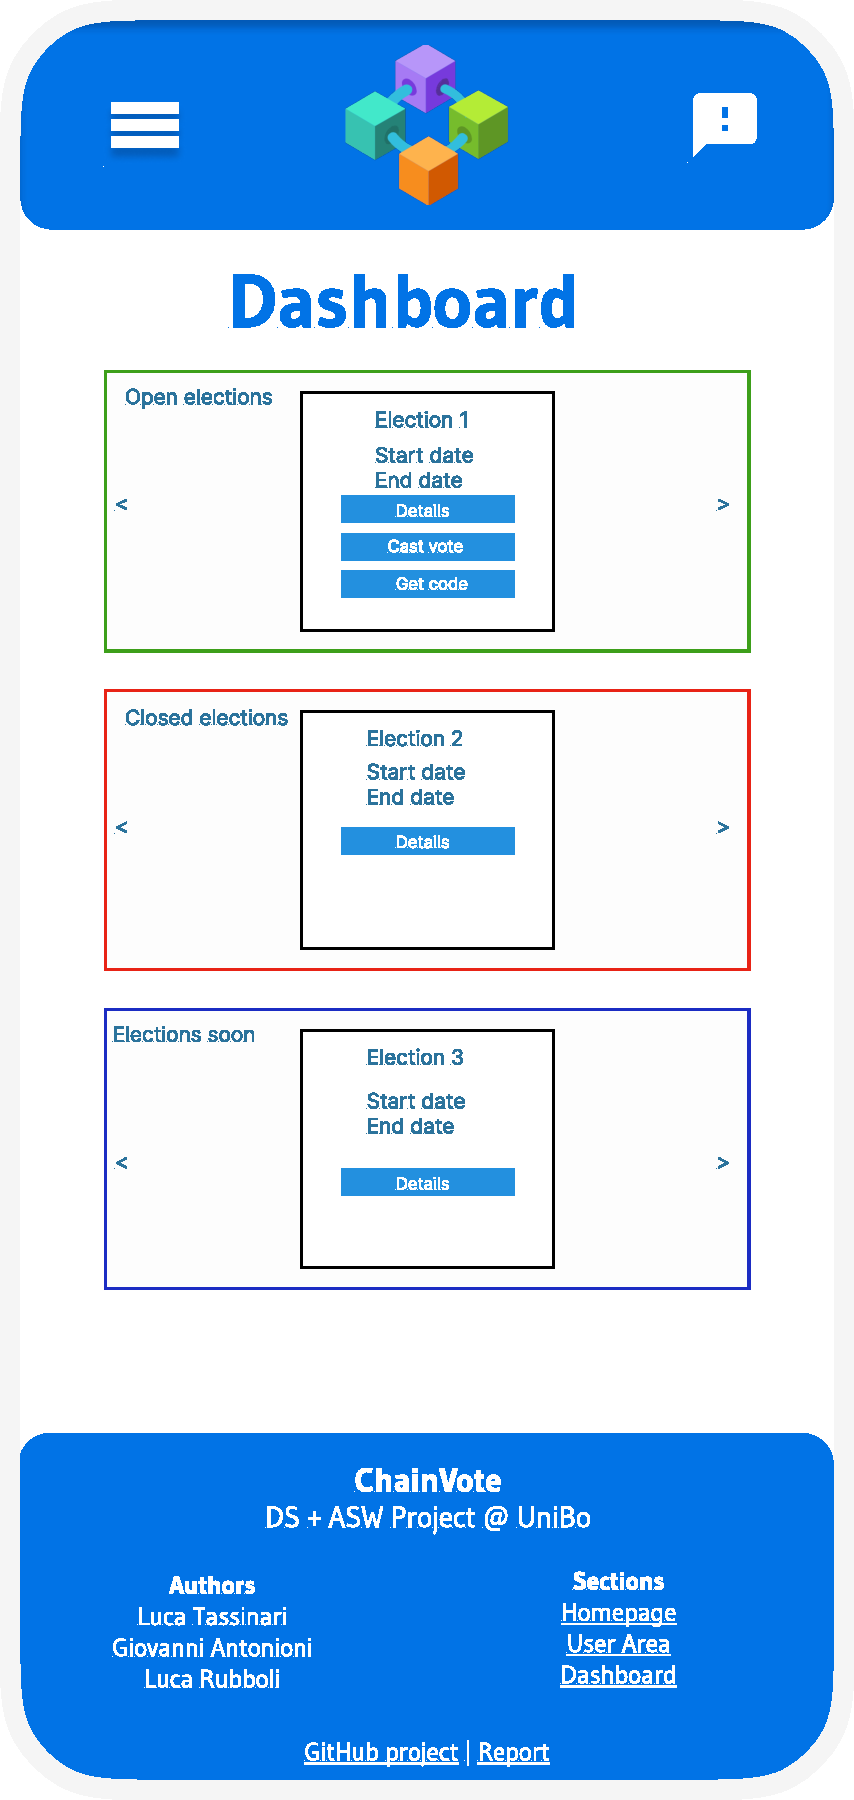
\includegraphics[width=\textwidth]{./figures/mockups/dashboard.pdf}
        %\caption{}
    \end{subfigure}
    \hfill
    \begin{subfigure}[b]{0.3\textwidth}
        \centering
        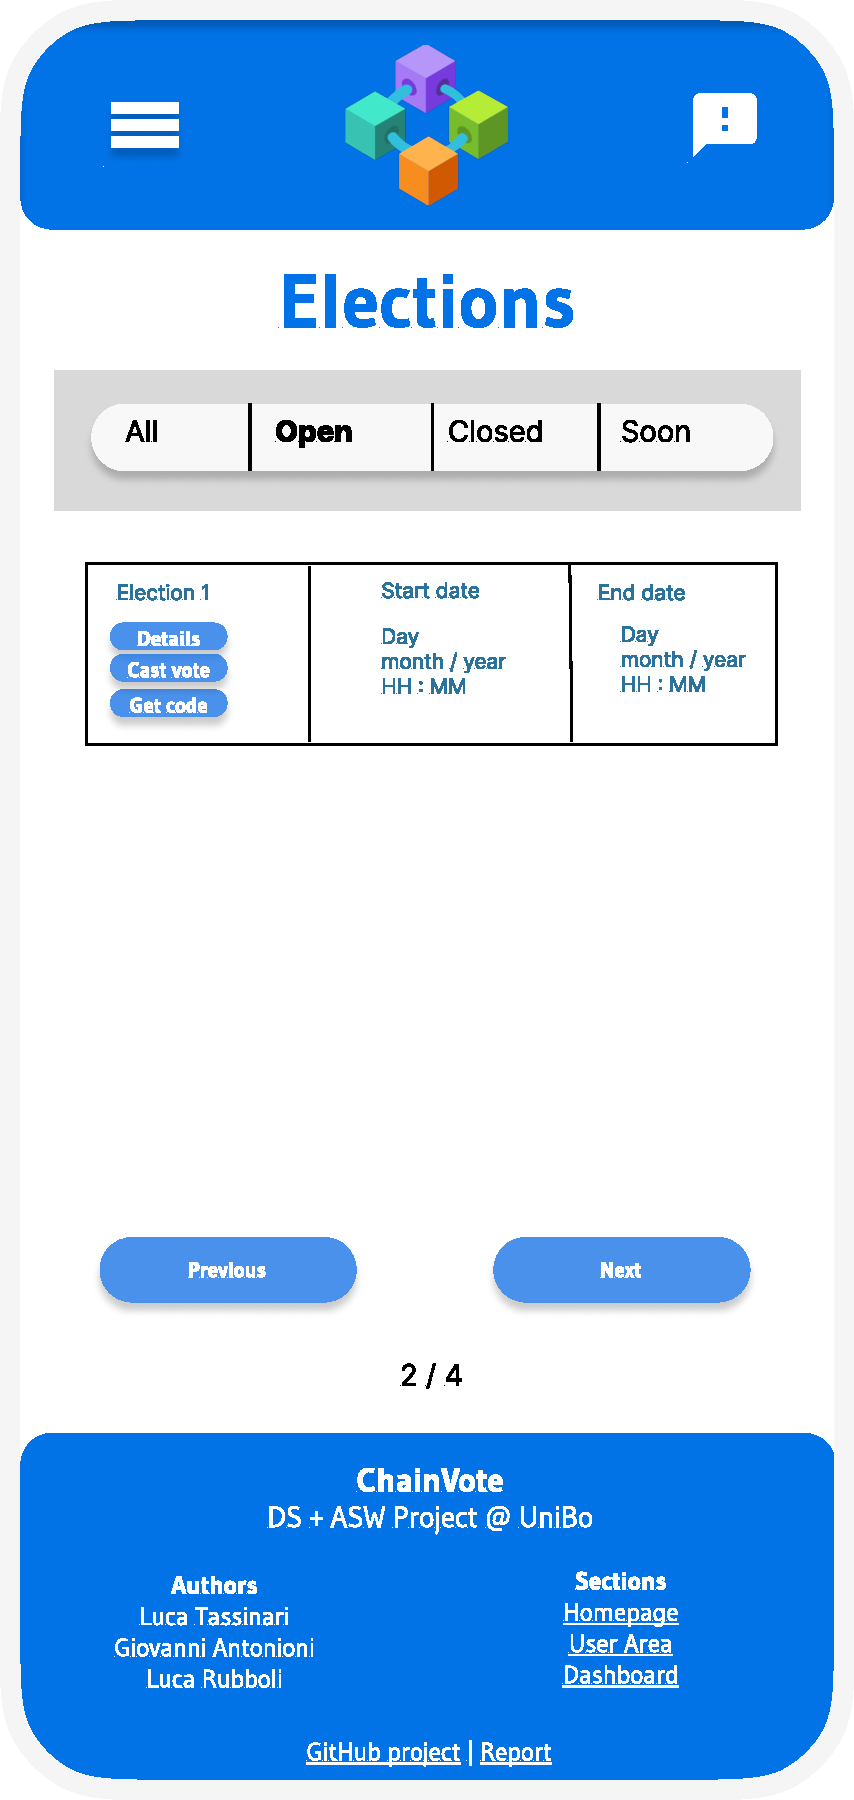
\includegraphics[width=\textwidth]{./figures/mockups/elections.pdf}
        %\caption{}
    \end{subfigure}
    \caption{Login, Dashboard and Elections views}
    \label{fig:login-dashboard-elections-views}
\end{figure}

\begin{figure}
    \centering
    \begin{subfigure}[b]{0.3\textwidth}
        \centering
        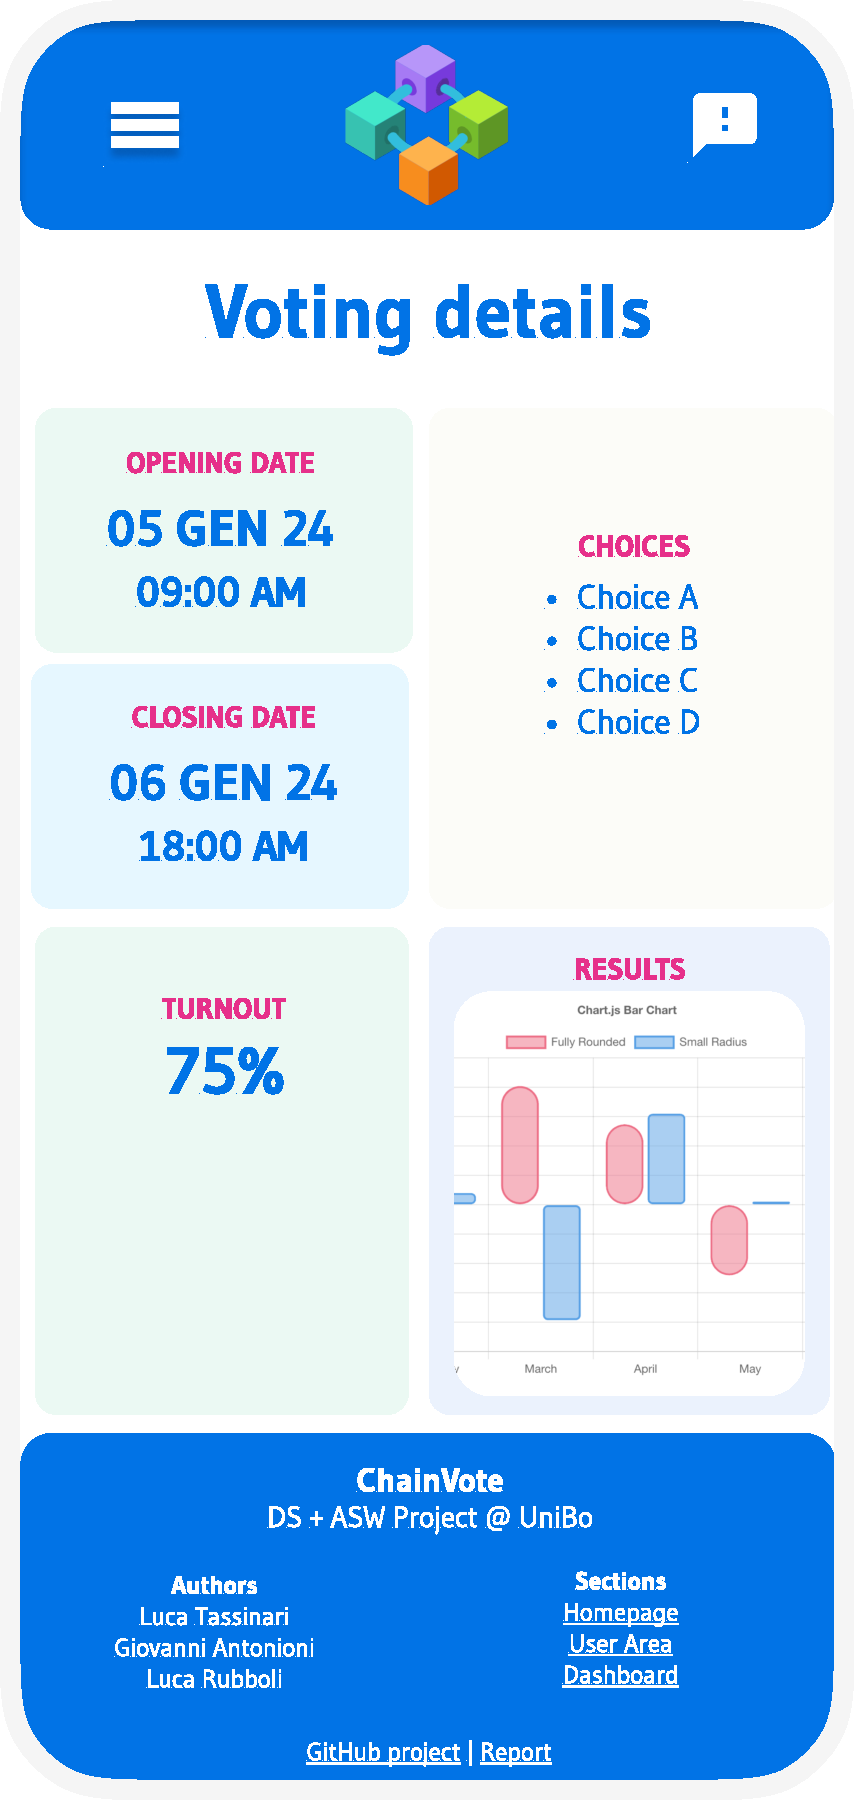
\includegraphics[width=\textwidth]{./figures/mockups/details.pdf}
        % \caption{}
    \end{subfigure}
    \hfill
    \begin{subfigure}[b]{0.3\textwidth}
        \centering
        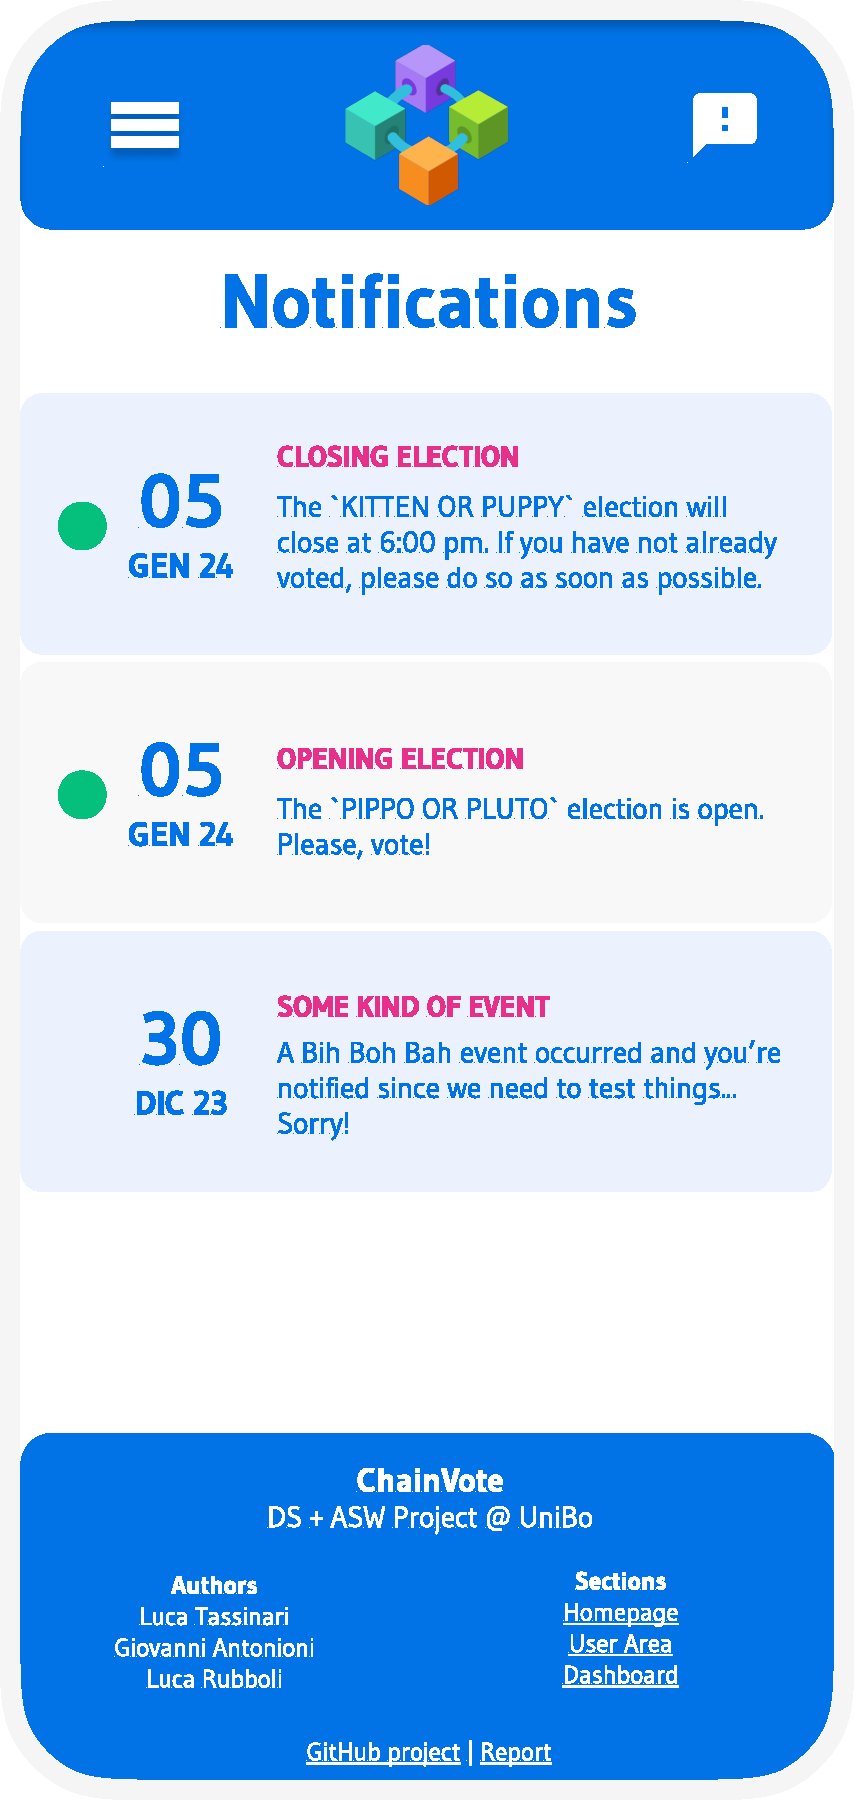
\includegraphics[width=\textwidth]{./figures/mockups/notifications.pdf}
        %\caption{}
    \end{subfigure}
    \hfill
    % add with subfigures the cast a vote view
    \caption{Voting details, Cast a vote and Notifications view.}
    \label{fig:details-cast-notifications-view}
\end{figure}
\todo{Cast a vote mockup}

\begin{figure}
    \begin{subfigure}[b]{0.3\textwidth}
        \centering
        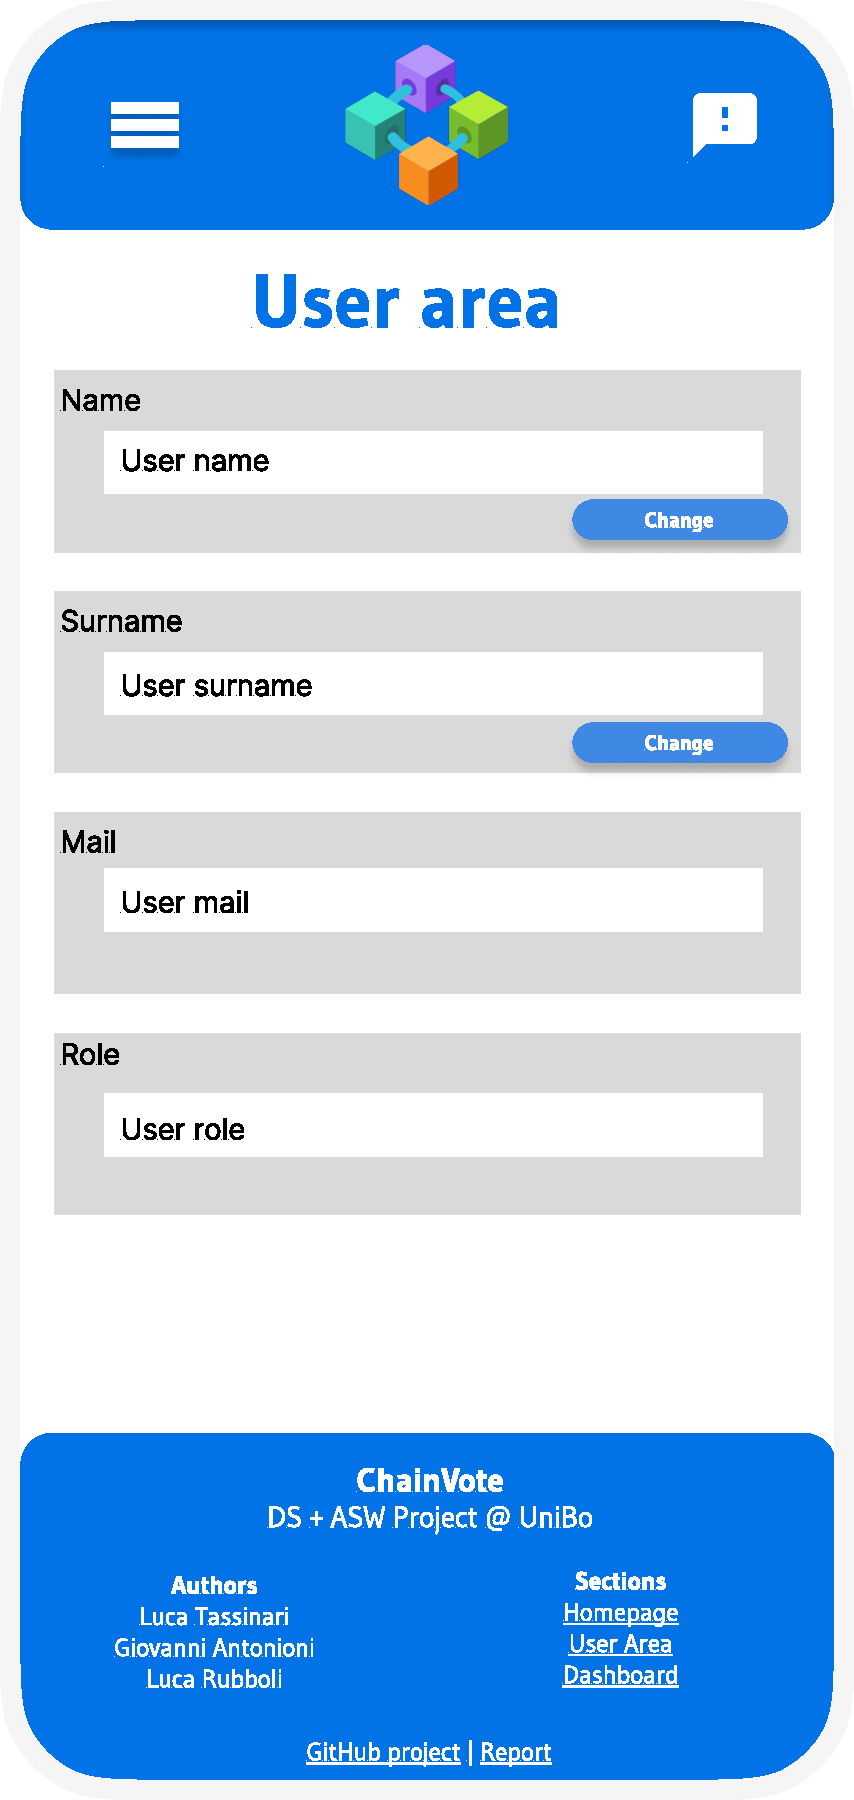
\includegraphics[width=\textwidth]{./figures/mockups/user-area.pdf}
        %\caption{}
    \end{subfigure}
    \caption{User area view.}
    \label{fig:user-area-view}
\end{figure}

\begin{figure}
    \begin{subfigure}[b]{0.3\textwidth}
        \centering
        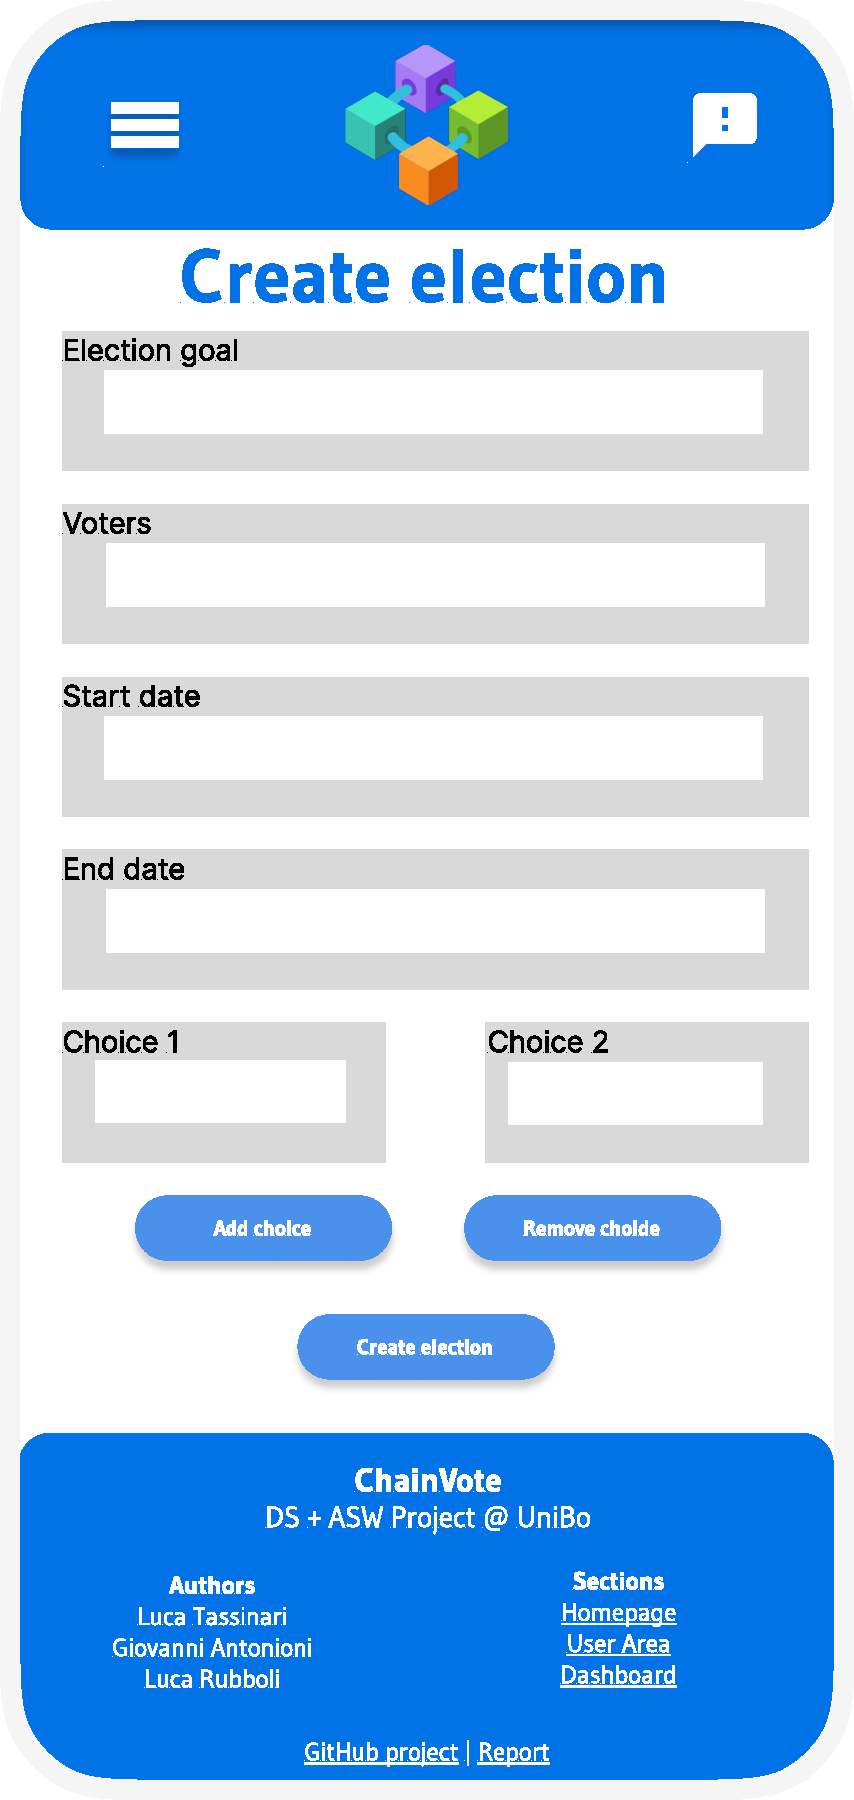
\includegraphics[width=\textwidth]{./figures/mockups/create-election.pdf}
        %\caption{}
    \end{subfigure}
    \caption{Create election view.}
    \label{fig:create-election-view}
\end{figure}

\subsection{Backend Architecture}

%% -------------------------------------- DS ----------------------------
\iffalse

The following section presents the blockchain network architecture, as well as that of the application.

\subsection{Blockchain architecture}
\label{subsec:blockchain-architecture}

In \Cref{fig:network-architecture} is shown the blockchain network architecture that has been conceived.

\begin{figure}
    \centering
    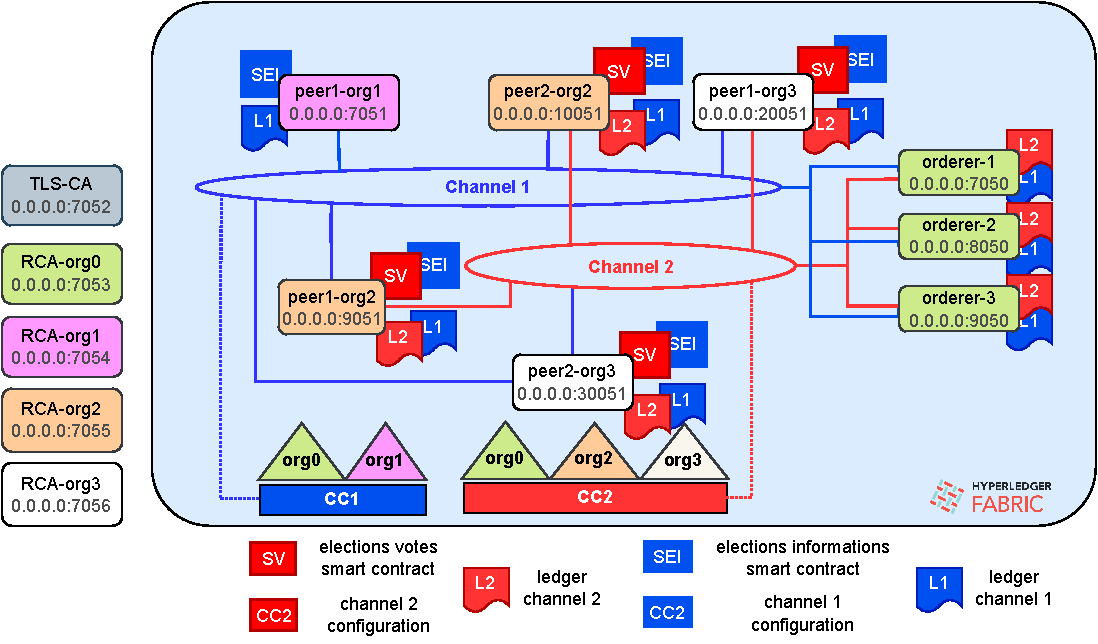
\includegraphics[width=\linewidth]{figures/network-architecture.pdf}
    \caption{High-level network architecture.}
    \label{fig:network-architecture}
\end{figure}

In total, four main organizations are in place:
\begin{itemize}
    \item one contains the orderer service (\texttt{org0});
    \item one in charge of creating and updating the elections' static information (\texttt{org1}), like a central governance institution. This information is stored inside the ledger of channel 1;
    \item two participating in the voting which maintains the vote-collecting functionalities and codes management (\texttt{org2} and \texttt{org3}) by means of querying static information when needed. This information is stored inside the ledger of channel 2.
\end{itemize} 

For the sake of fault tolerance both \texttt{org2} and \texttt{org3} contain two peers each, while the orderer service (\texttt{org0}) contains three orderer nodes.

As already said above, as a permissioned blockchain, Hyperledger Fabric requires all the entities to be identified. This is implemented through digital certificates, managed by specific infrastructures that deal with their issuance.
Those infrastructures are the certificate authorities:

\begin{itemize}
    \item \textbf{RCA-org\emph{x}} ($x$=0,1,2,3) is the Root CA for identities in each organization; it issues identity-related certificates for components and users and provides MSP functionalities during the network configuration phase.
    \item \textbf{TLS-CA} issuing TLS server certificates for network components (orderer and peers) for the whole network. This certification is for TLS communication only, and not related to identity in this fabric network. Concretely, when a client accesses a network component it will present its own TLS server certificate to the client. The client will use the Root CA certificate to verify the server one, and confirm the client is talking to the right server and that the communication is encrypted.
\end{itemize}

Once the certificate issuance is done and the network is set up, certificate authorities are used only in case new components or new users join the network.

\begin{warn}[\textit{Warning}]
    This is just a proof of concept of what a real blockchain network for an electronic voting system should look like. For example, it is obvious that, in a real scenario, there would be a higher number of orderer nodes allowing the system to tolerate a much higher number of failures (with the presented architecture we tolerate only one failure). 
    The simplification is necessitated by the fact that the entire network will be deployed on a single machine using containerization tools, in which for each node (and for each smart contract) a container is created.
    Simulating a real blockchain network would mean running a large number of containers, which would make the deployment very computationally expensive.
\end{warn}

\subsection{Application abstract design}

\subsubsection{Structure / Domain Entities}

\subparagraph*{Elections}

As shown in \Cref{fig:election-design}, the core entities involved in election management are:
\begin{itemize}
    \item \texttt{Election}, representing the election's vote information entity;
    \item \texttt{ElectionInfo}, representing the election's static information entity;
    \item \texttt{Ballot}, representing the vote entity;
    \item \texttt{Builders} entities to strengthen the control over features in the building phase;
    \item \texttt{ElectionFactory} is the interface that hides the verbosity of builders;
    \item \texttt{ElectionManager} is the interface exposing method to manage the vote-casting process, including all verifications.
\end{itemize}

\subparagraph*{Codes}

In \Cref{fig:codes-design} are summarized the main entities of the domain model concerning codes management.
%
In particular:
%
\begin{itemize}
    \item \texttt{OneTimeCode} represents the one time code entity;
    \item \texttt{CodesGeneratorStrategy} represents the strategy (i.e. the algorithm) used to generate the codes;
    \item \texttt{CodesRepository} is the interface managing the storage and retrieval of the codes. This interface is agnostic of the storage technology and will possibly be implemented in several ways, depending on the adopted one.
    \item \texttt{CodesManager} is the interface exposing methods to manage the creation, verification and (in)validation of codes. 
\end{itemize}

\begin{landscape}
    \begin{figure}
        \centering
        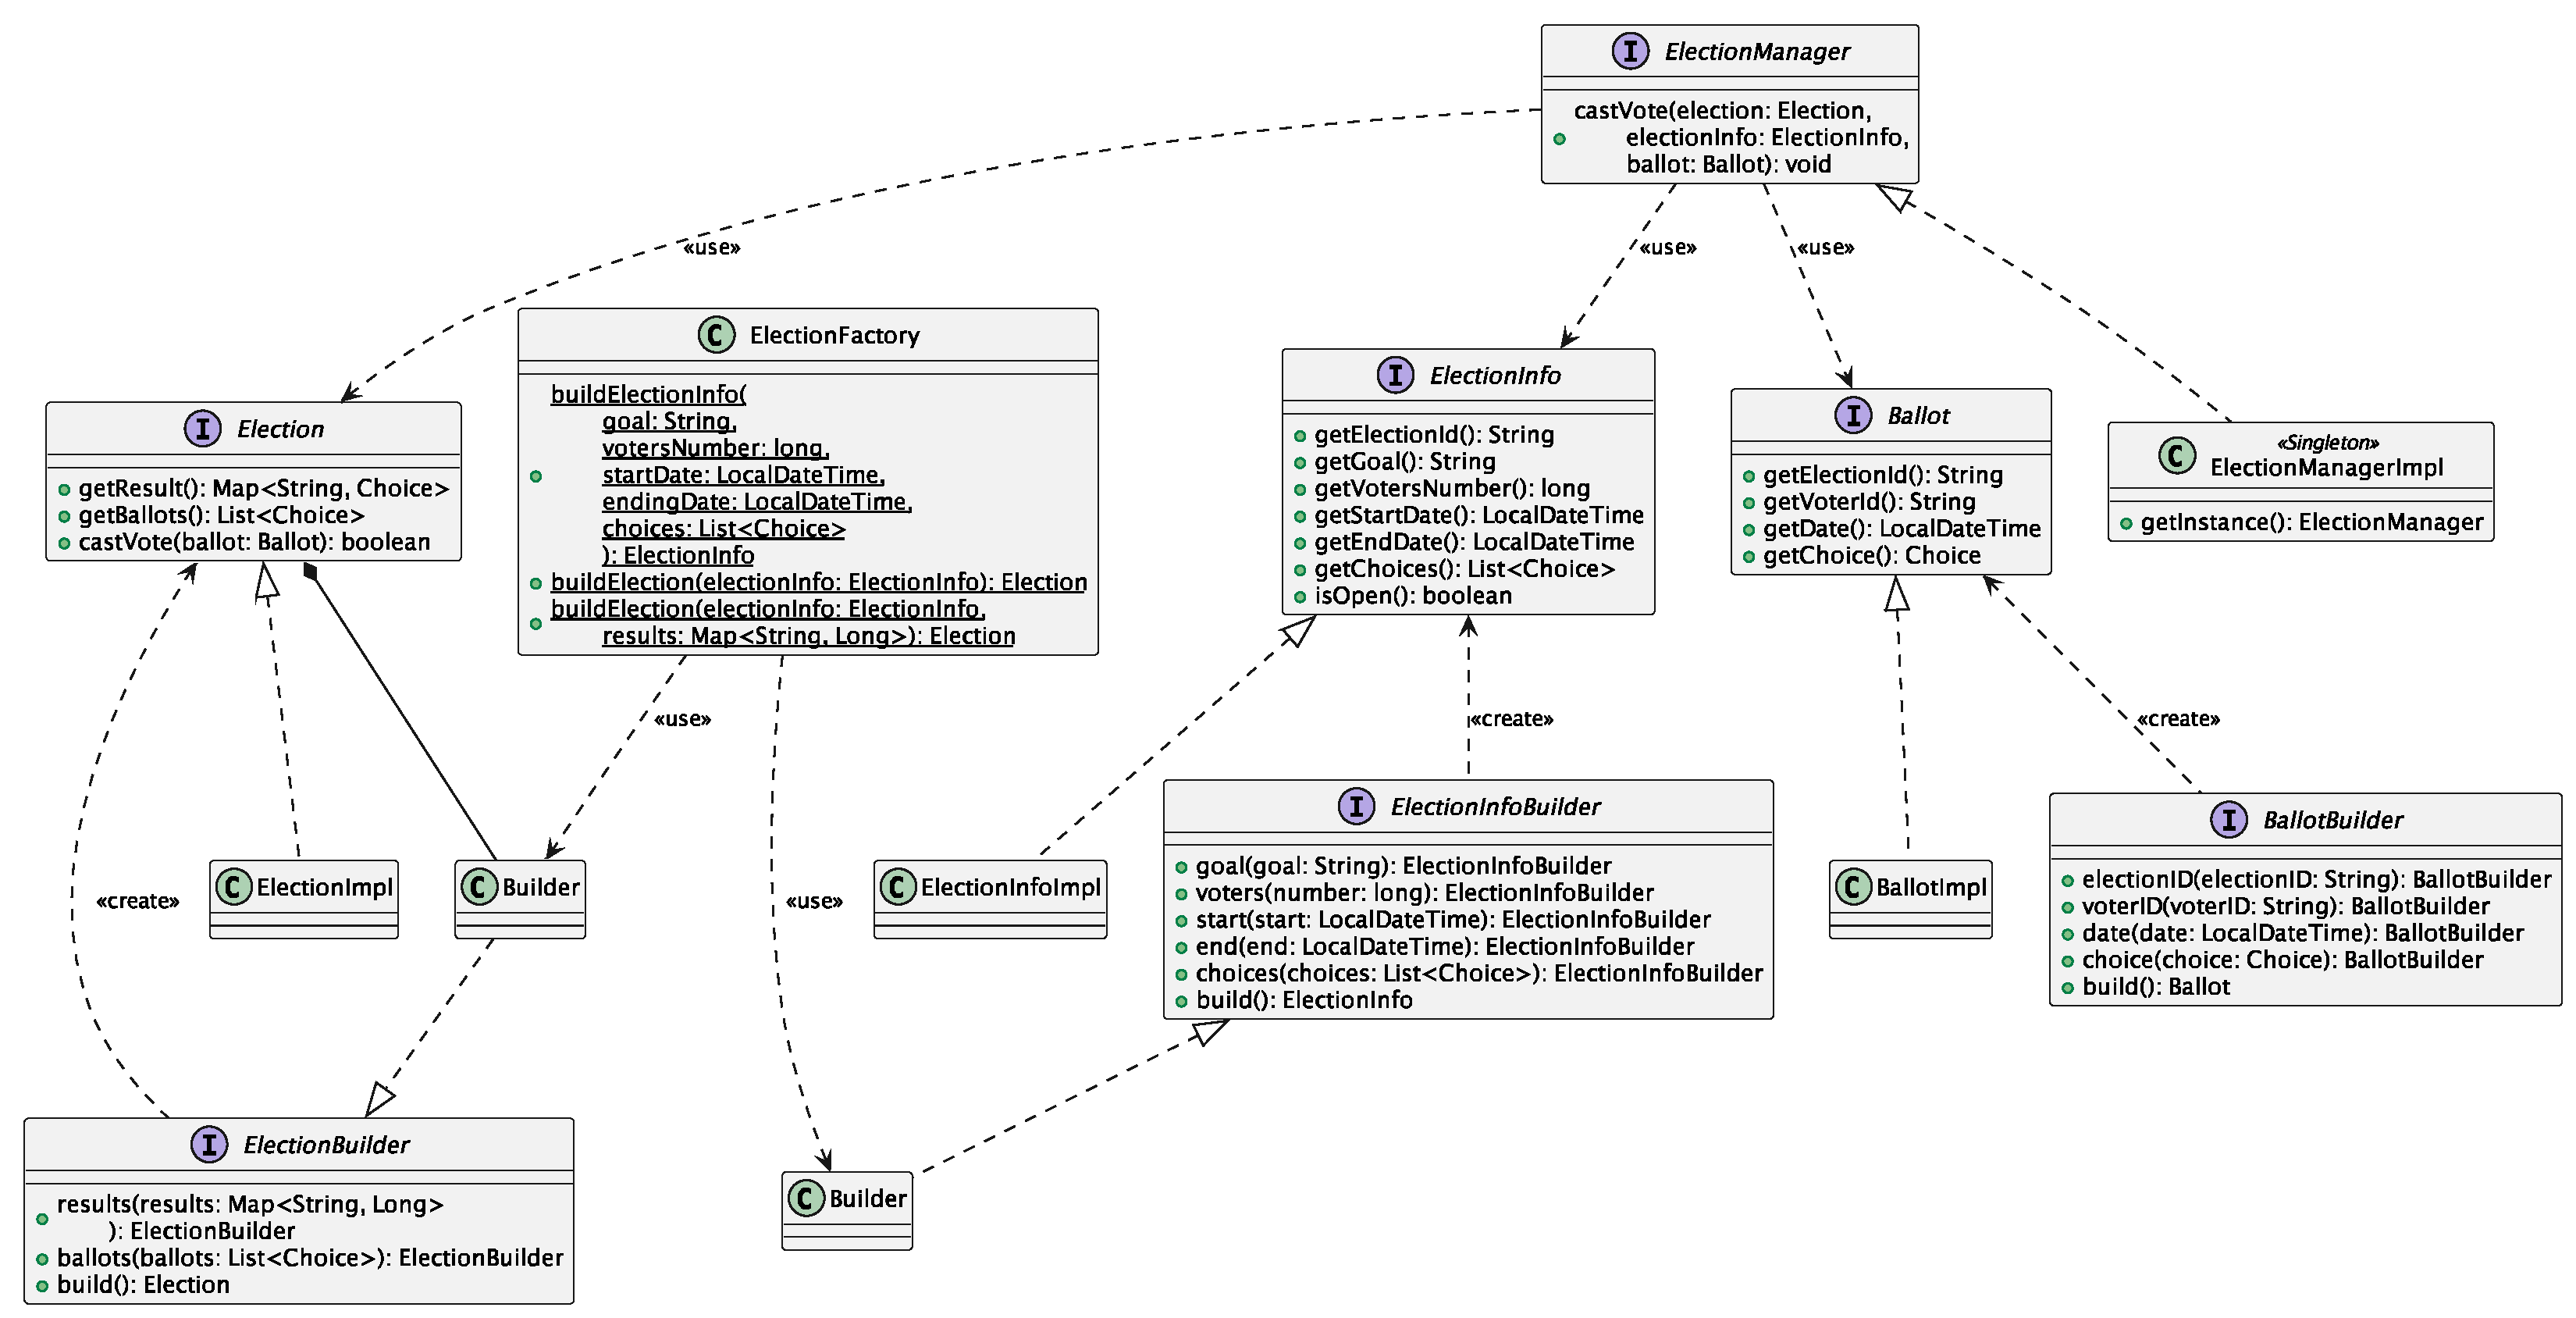
\includegraphics[width=\linewidth]{figures/election-design.eps}
        \caption{UML class diagram of the election's domain entities.}
        \label{fig:election-design} 
    \end{figure}
\end{landscape}

\begin{figure}
    \centering
    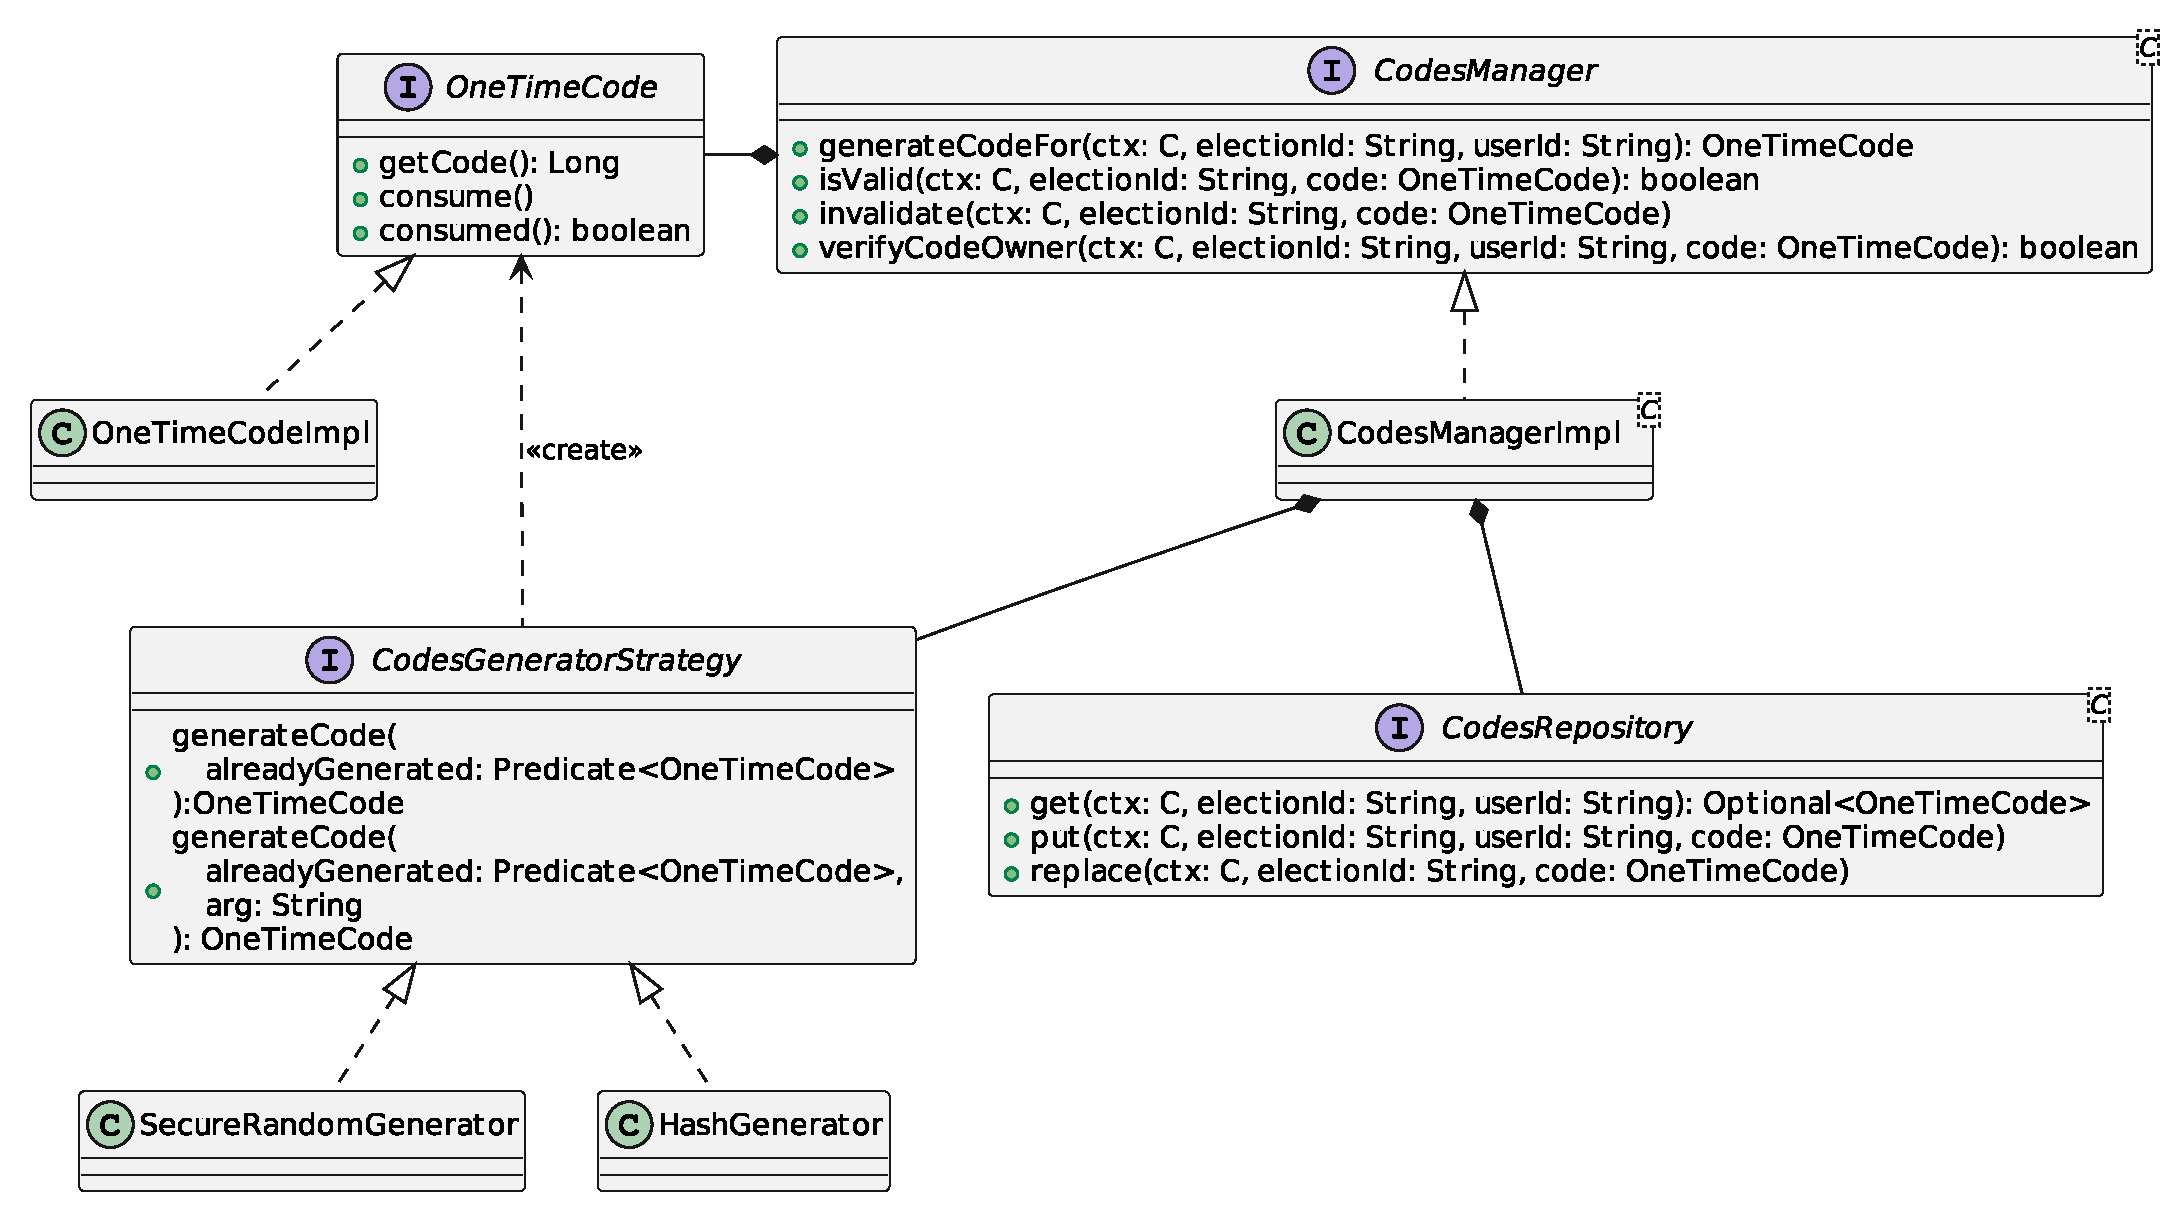
\includegraphics[width=\linewidth]{figures/codes-design.eps}
    \caption{UML class diagram of the code's domain entities.}
    \label{fig:codes-design} 
\end{figure}

\subsubsection{Interaction}

In the following section are presented the most relevant (non-trivial) interactions grouped by use cases.

\subparagraph*{Use case: authentication to the system}
\label{uc:auth-to-the-system} 
To interact with the system a user must request an authentication token from the server first (see \Cref{fig:login-to-the-system}). To do this it must provide a valid username and password, then the server will check if the account exists and if the password is correct.
If authentication is successful, the server will sign a pair of JWT tokens and send them to the user. These two will fill two distinct roles:
\begin{itemize}
    \item \textbf{access token}: is needed to authenticate the user's requests to the system;
    \item \textbf{refresh token}: is needed to renew authentication without the user passing his credentials again.
\end{itemize}
Both must be stored securely once they have been transmitted. The access token has a short lifetime, while the refresh token has a longer one. When the access token expires, the user must request a new one using the refresh token. If the refresh token expires, the user must log in again.

\begin{figure}
    \centering
    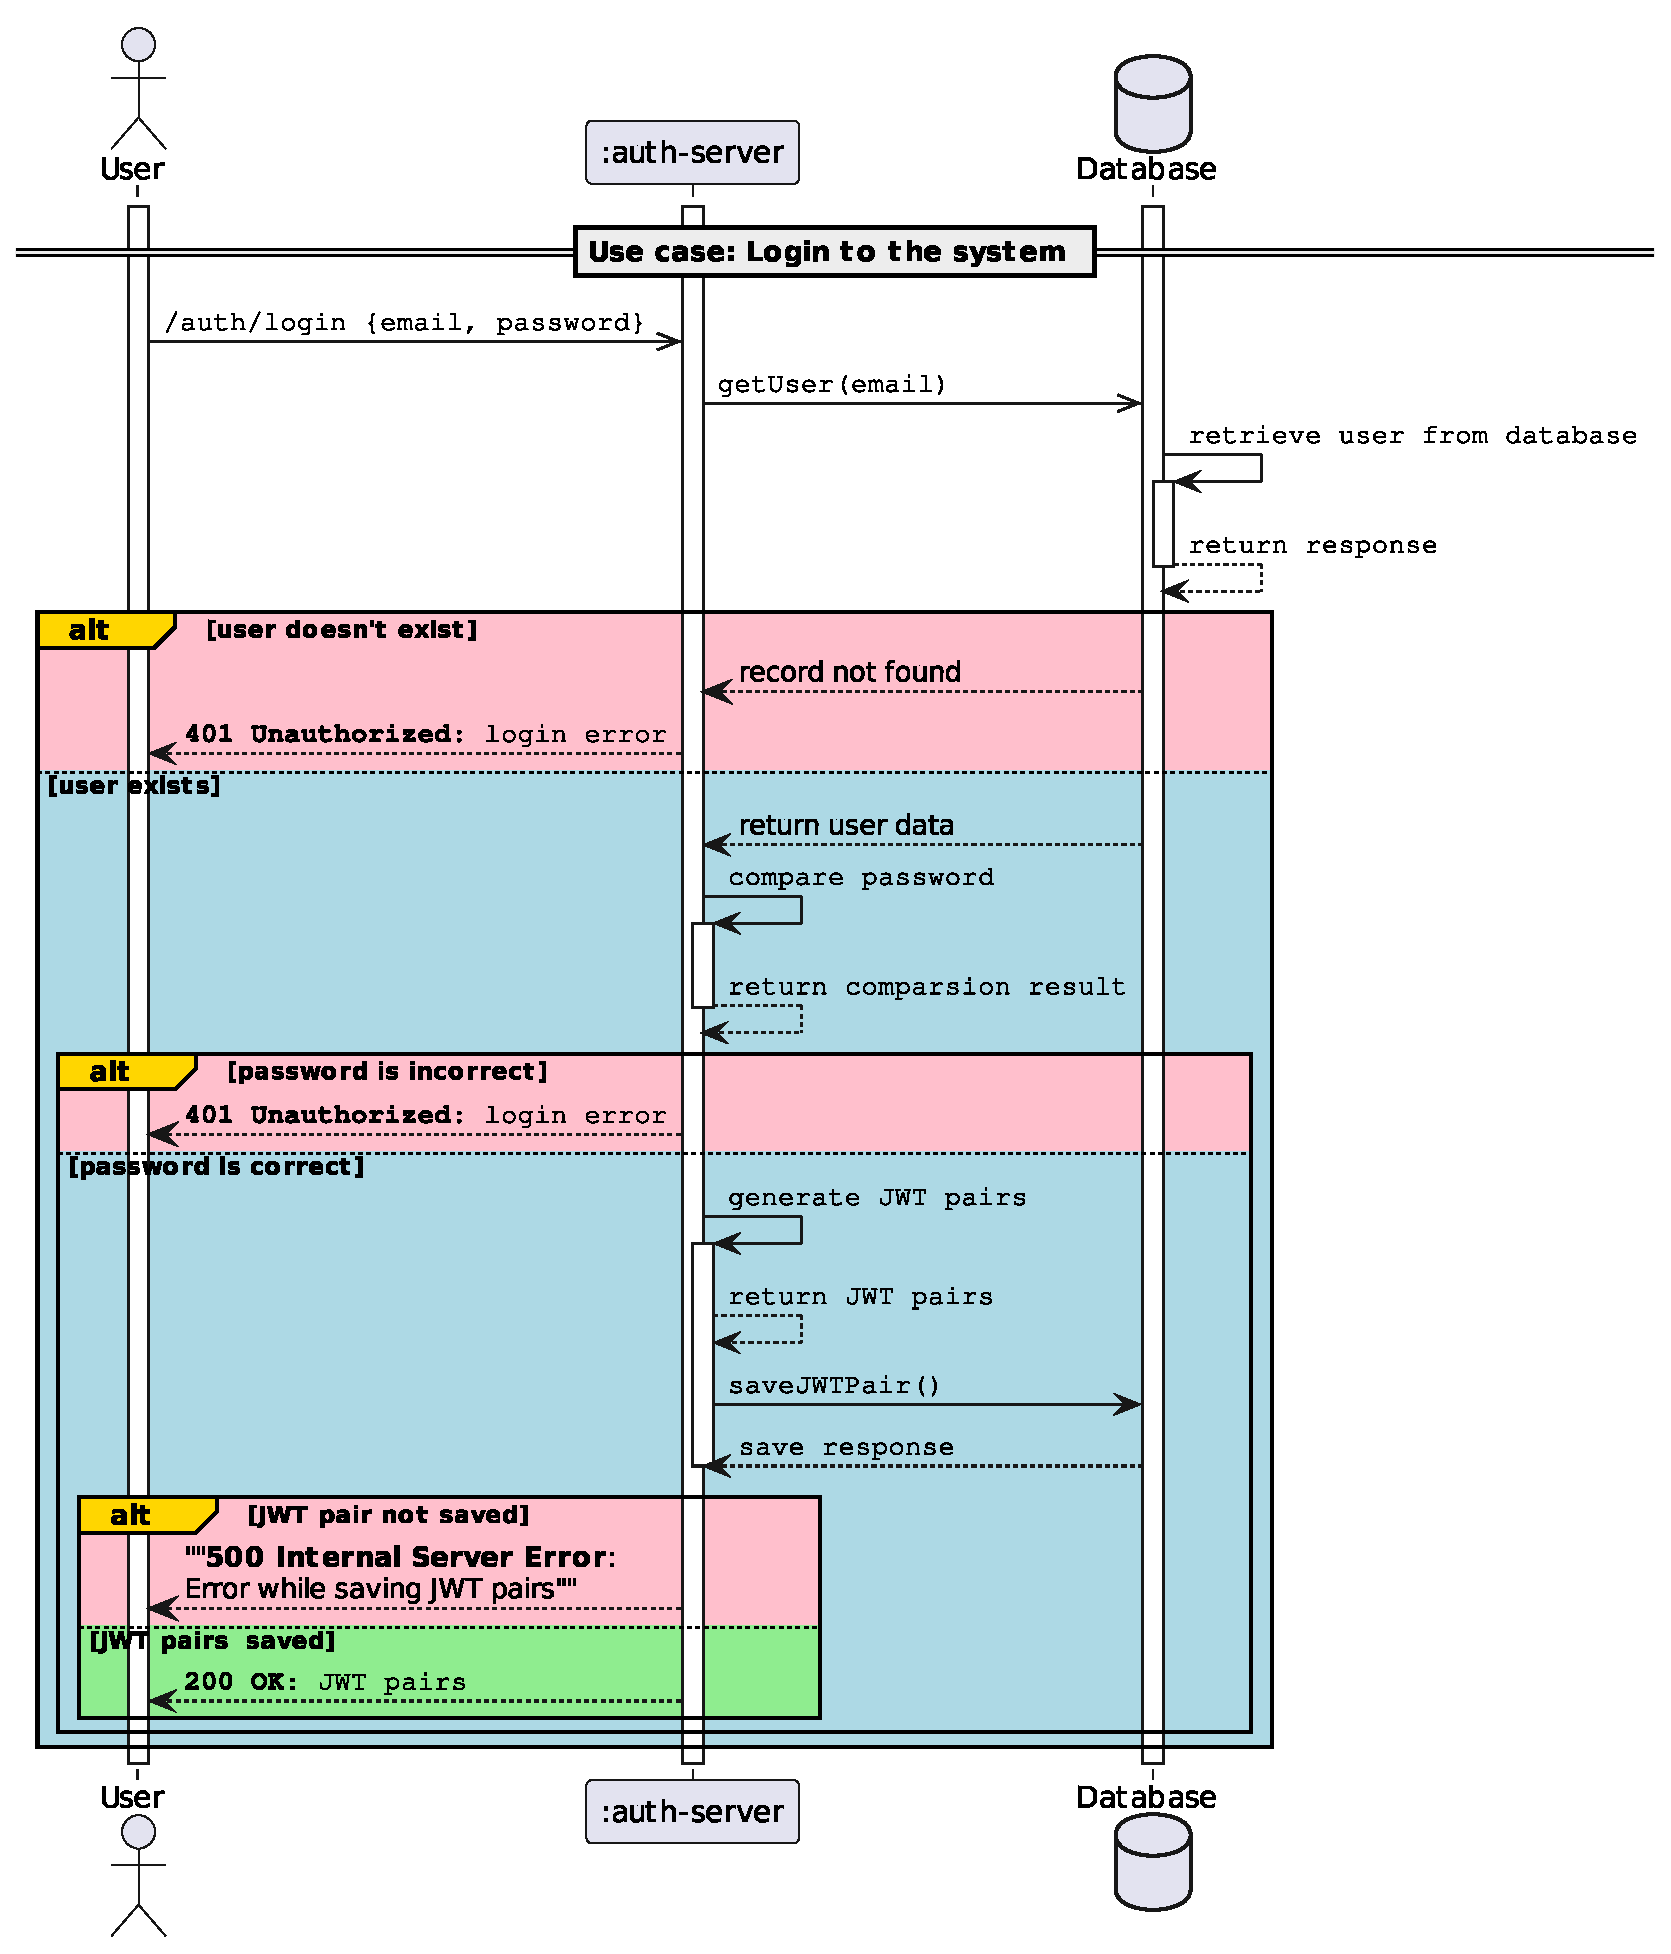
\includegraphics[width=\linewidth]{figures/login-to-the-system.eps}
    \caption{UML sequence diagram for the login use case.}
    \label{fig:login-to-the-system} 
\end{figure}

\subparagraph*{Use case: casting a new vote for a given election}

To cast a new vote, the user first requests the generation of a new one-time code for a specific election.
%
At the blockchain level, some checks are then performed in order to guarantee the election exists and a code has not already been generated for that user for the given election.
%
Once the code has been generated, the API server is in charge of transmitting it to the user (using a trusted method) (see \Cref{fig:code-creation-use-case}).
%
\begin{figure}
    \centering
    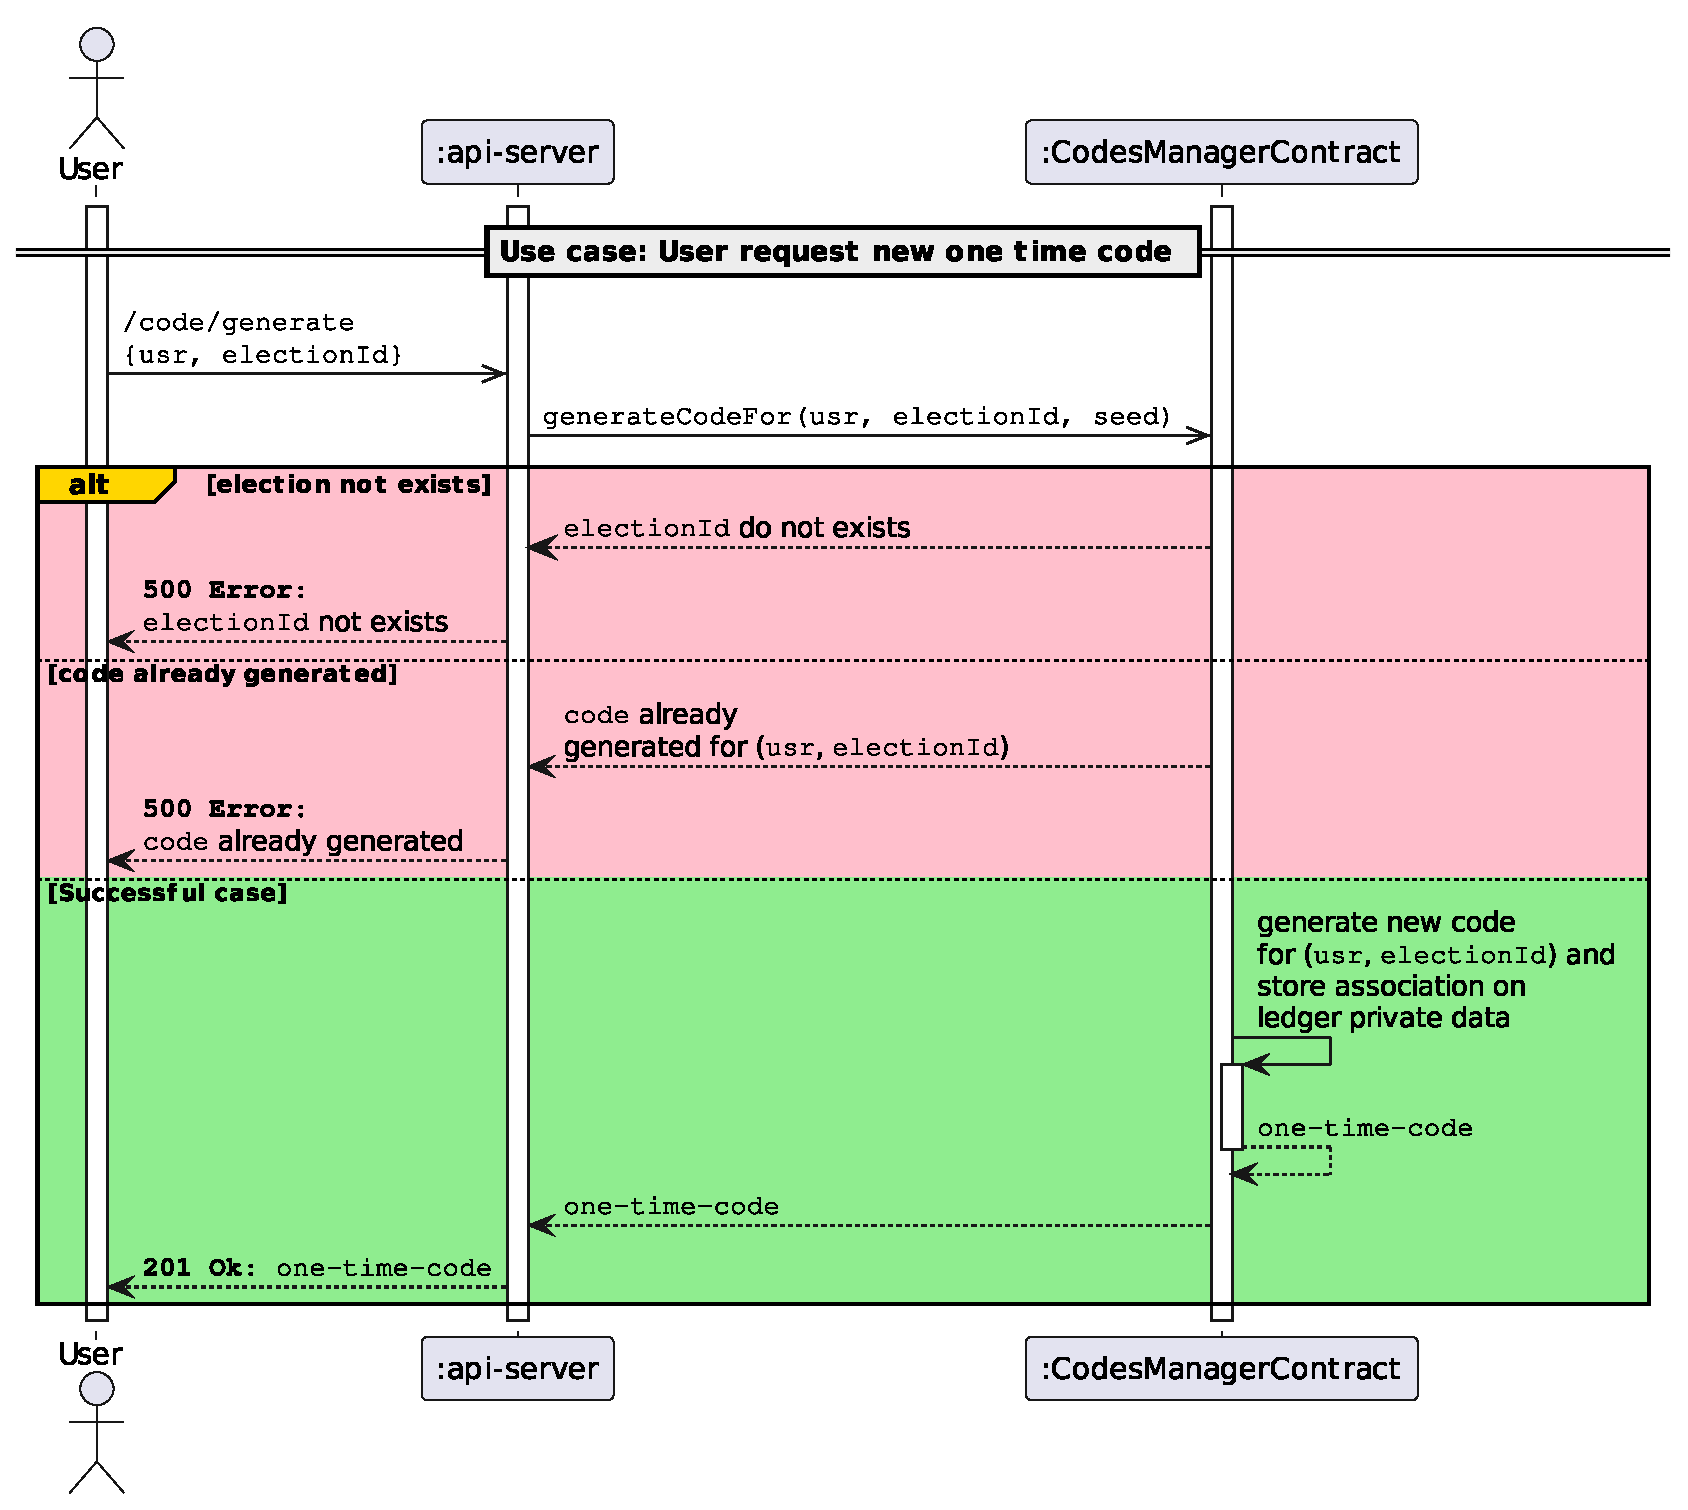
\includegraphics[width=\linewidth]{figures/code-creation-use-case.eps}
    \caption{UML sequence diagram for the code's request use case.}
    \label{fig:code-creation-use-case} 
\end{figure}
%
Upon receiving the code the user can cast their vote.
%
Again, at the smart contract level, several checks are performed in order to ensure that the writing to the ledger of the newly cast vote is successful only if the election is open and the code is still valid, i.e. it is associated with the user who is requesting to vote and has not already been used. 
%
Finally, the code is invalidated (see \Cref{fig:cast-vote-use-case}).
%
The fact the code check and its invalidation are performed within the smart contracts of the blockchain ensures that it either succeeds and all peers agree on that or fails and the transaction is not recorded into the ledger. 
%
If these two actions were invoked from the API service a crash of the server in between a successful cast and code invalidation may allow the user to cast, at least theoretically, an infinite number of times, unless appropriately managed.

\begin{figure}[h!]
    \centering
    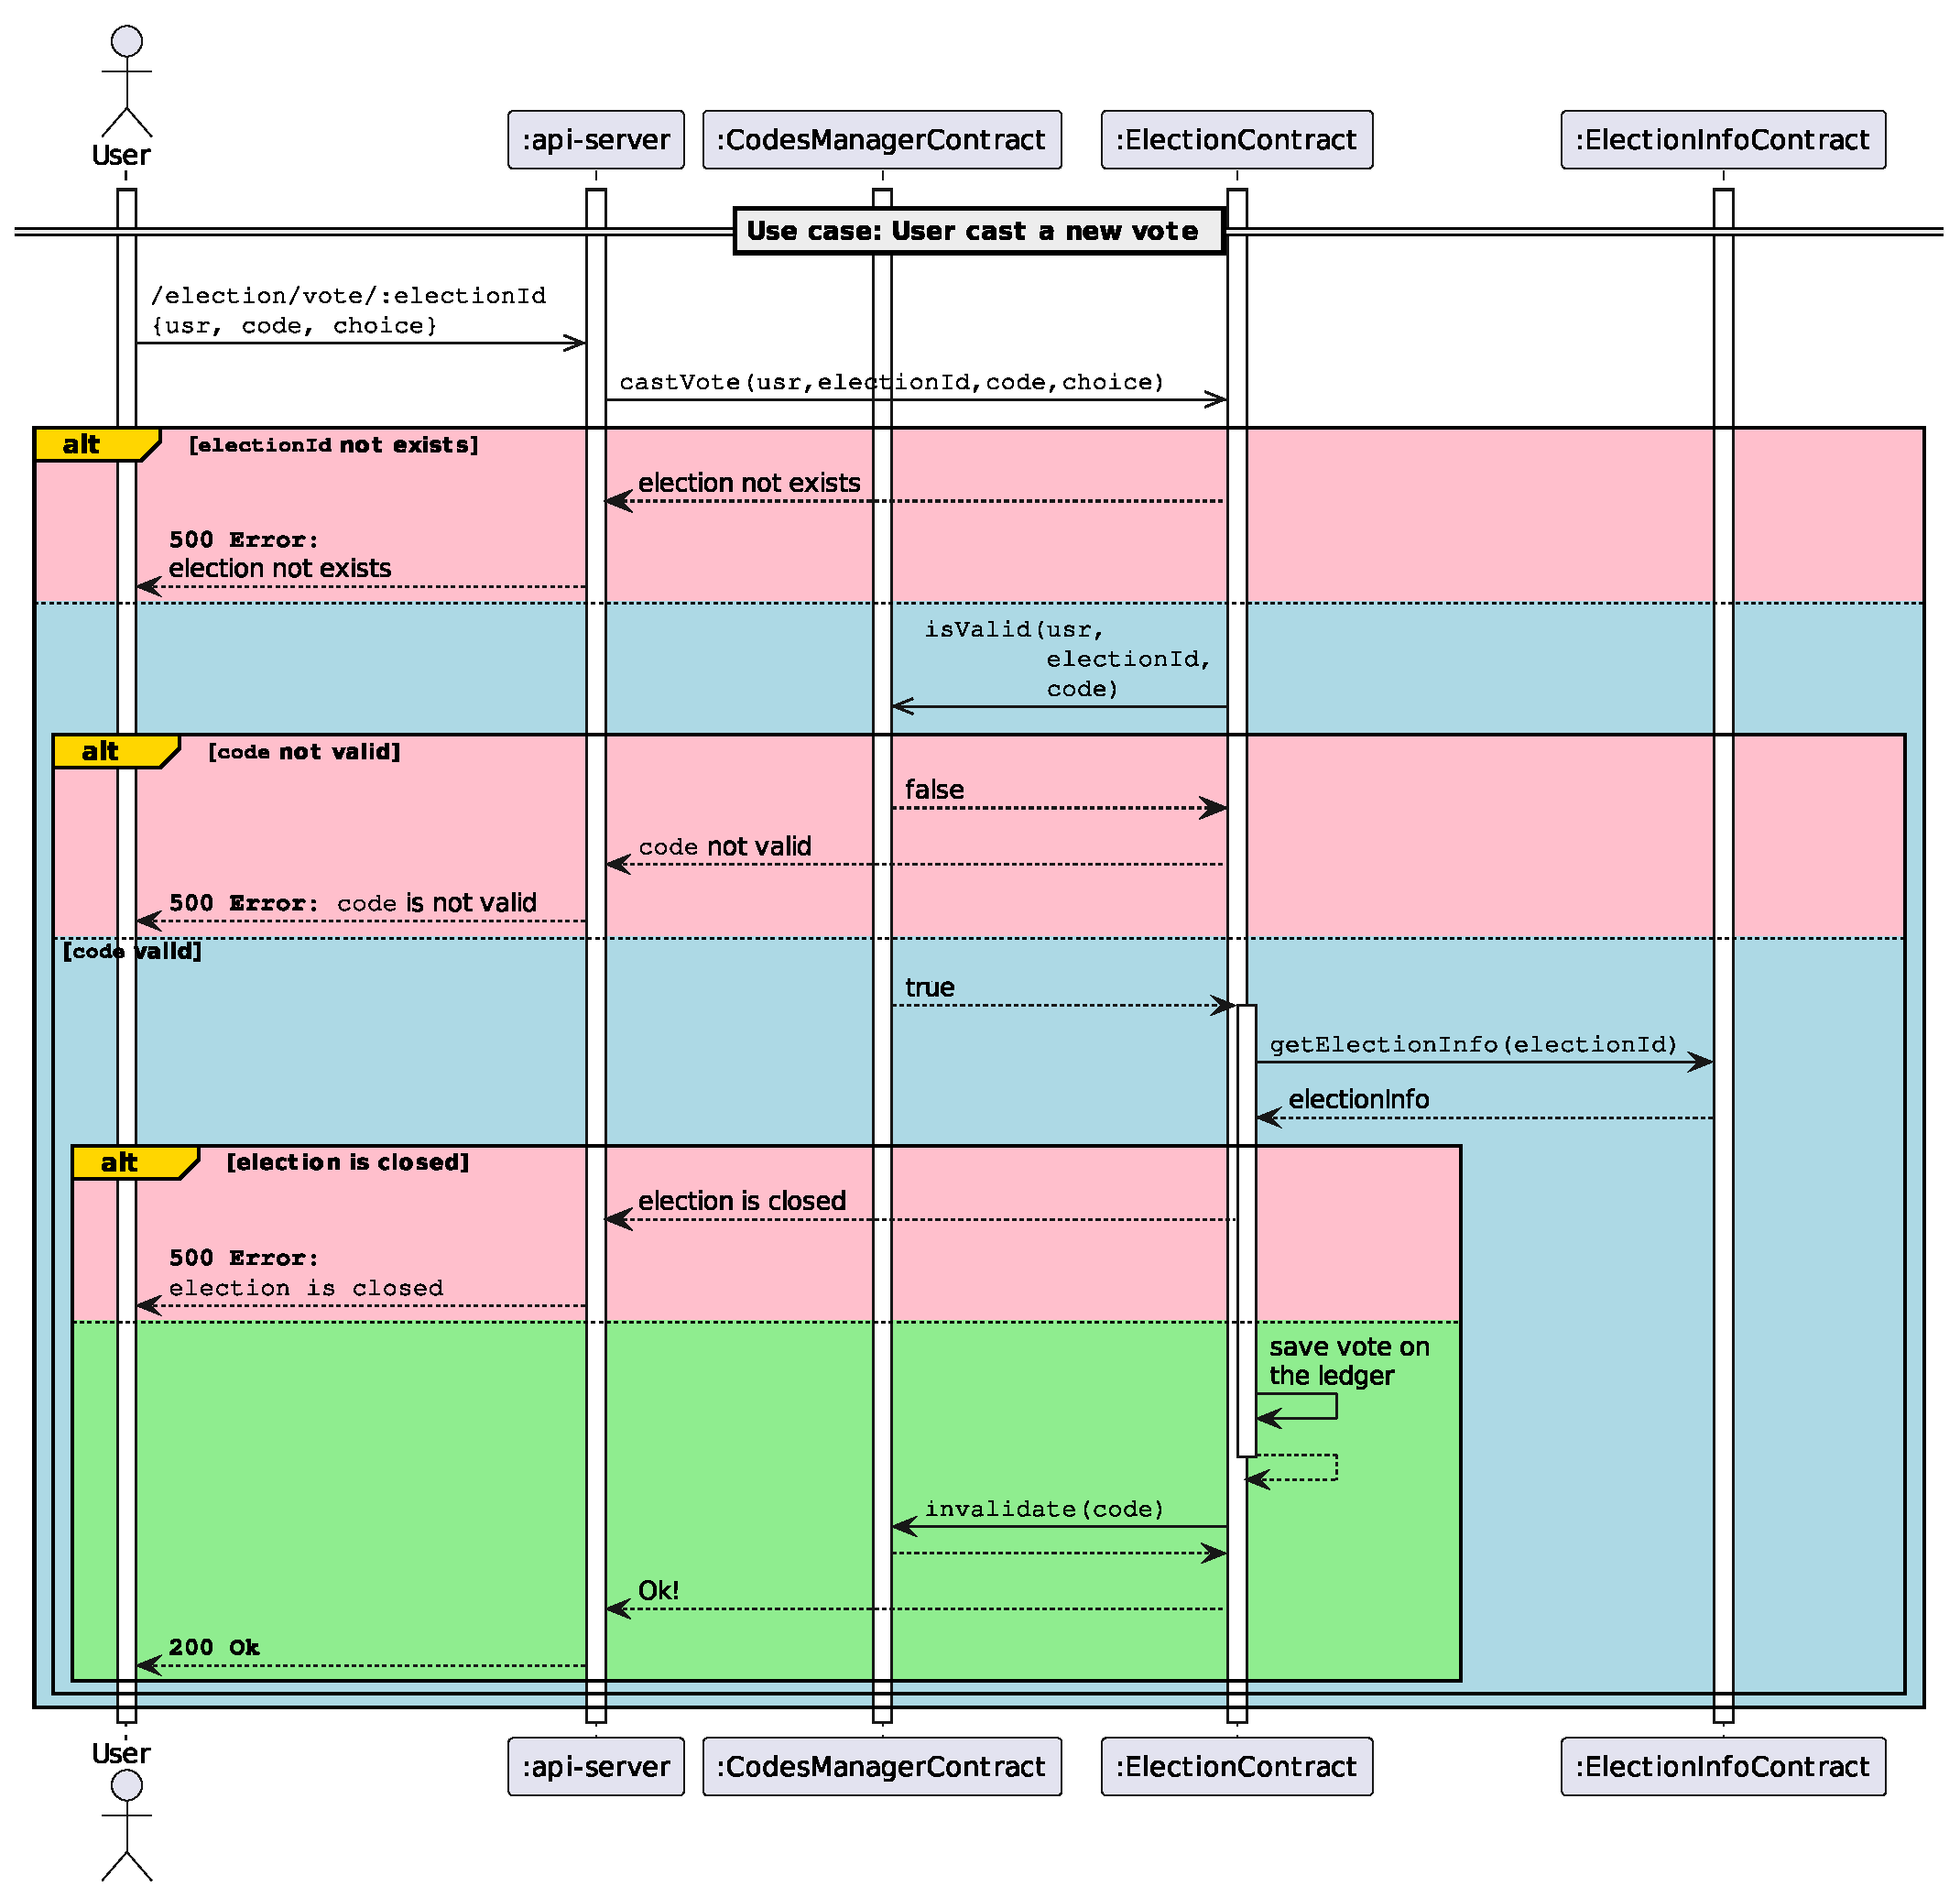
\includegraphics[width=\linewidth]{figures/cast-vote-use-case.eps}
    \caption{UML sequence diagram for the vote casting use case.}
    \label{fig:cast-vote-use-case} 
\end{figure}

\subsection{Architectural design}

The architecture of the system is composed of three main components (see \Cref{fig:system-architecture}):
\begin{itemize}
    \item \texttt{:blockchain} component is in charge of the configuration and creation of the network's artifacts, as well as its deployment.
    \item \texttt{:api-service} module exposes the API to interact with the system. 
    \item \texttt{:smart-contracts} module contains the implementation of the blockchain smart contracts.
\end{itemize}

\begin{landscape}
    \begin{figure}
        \centering
        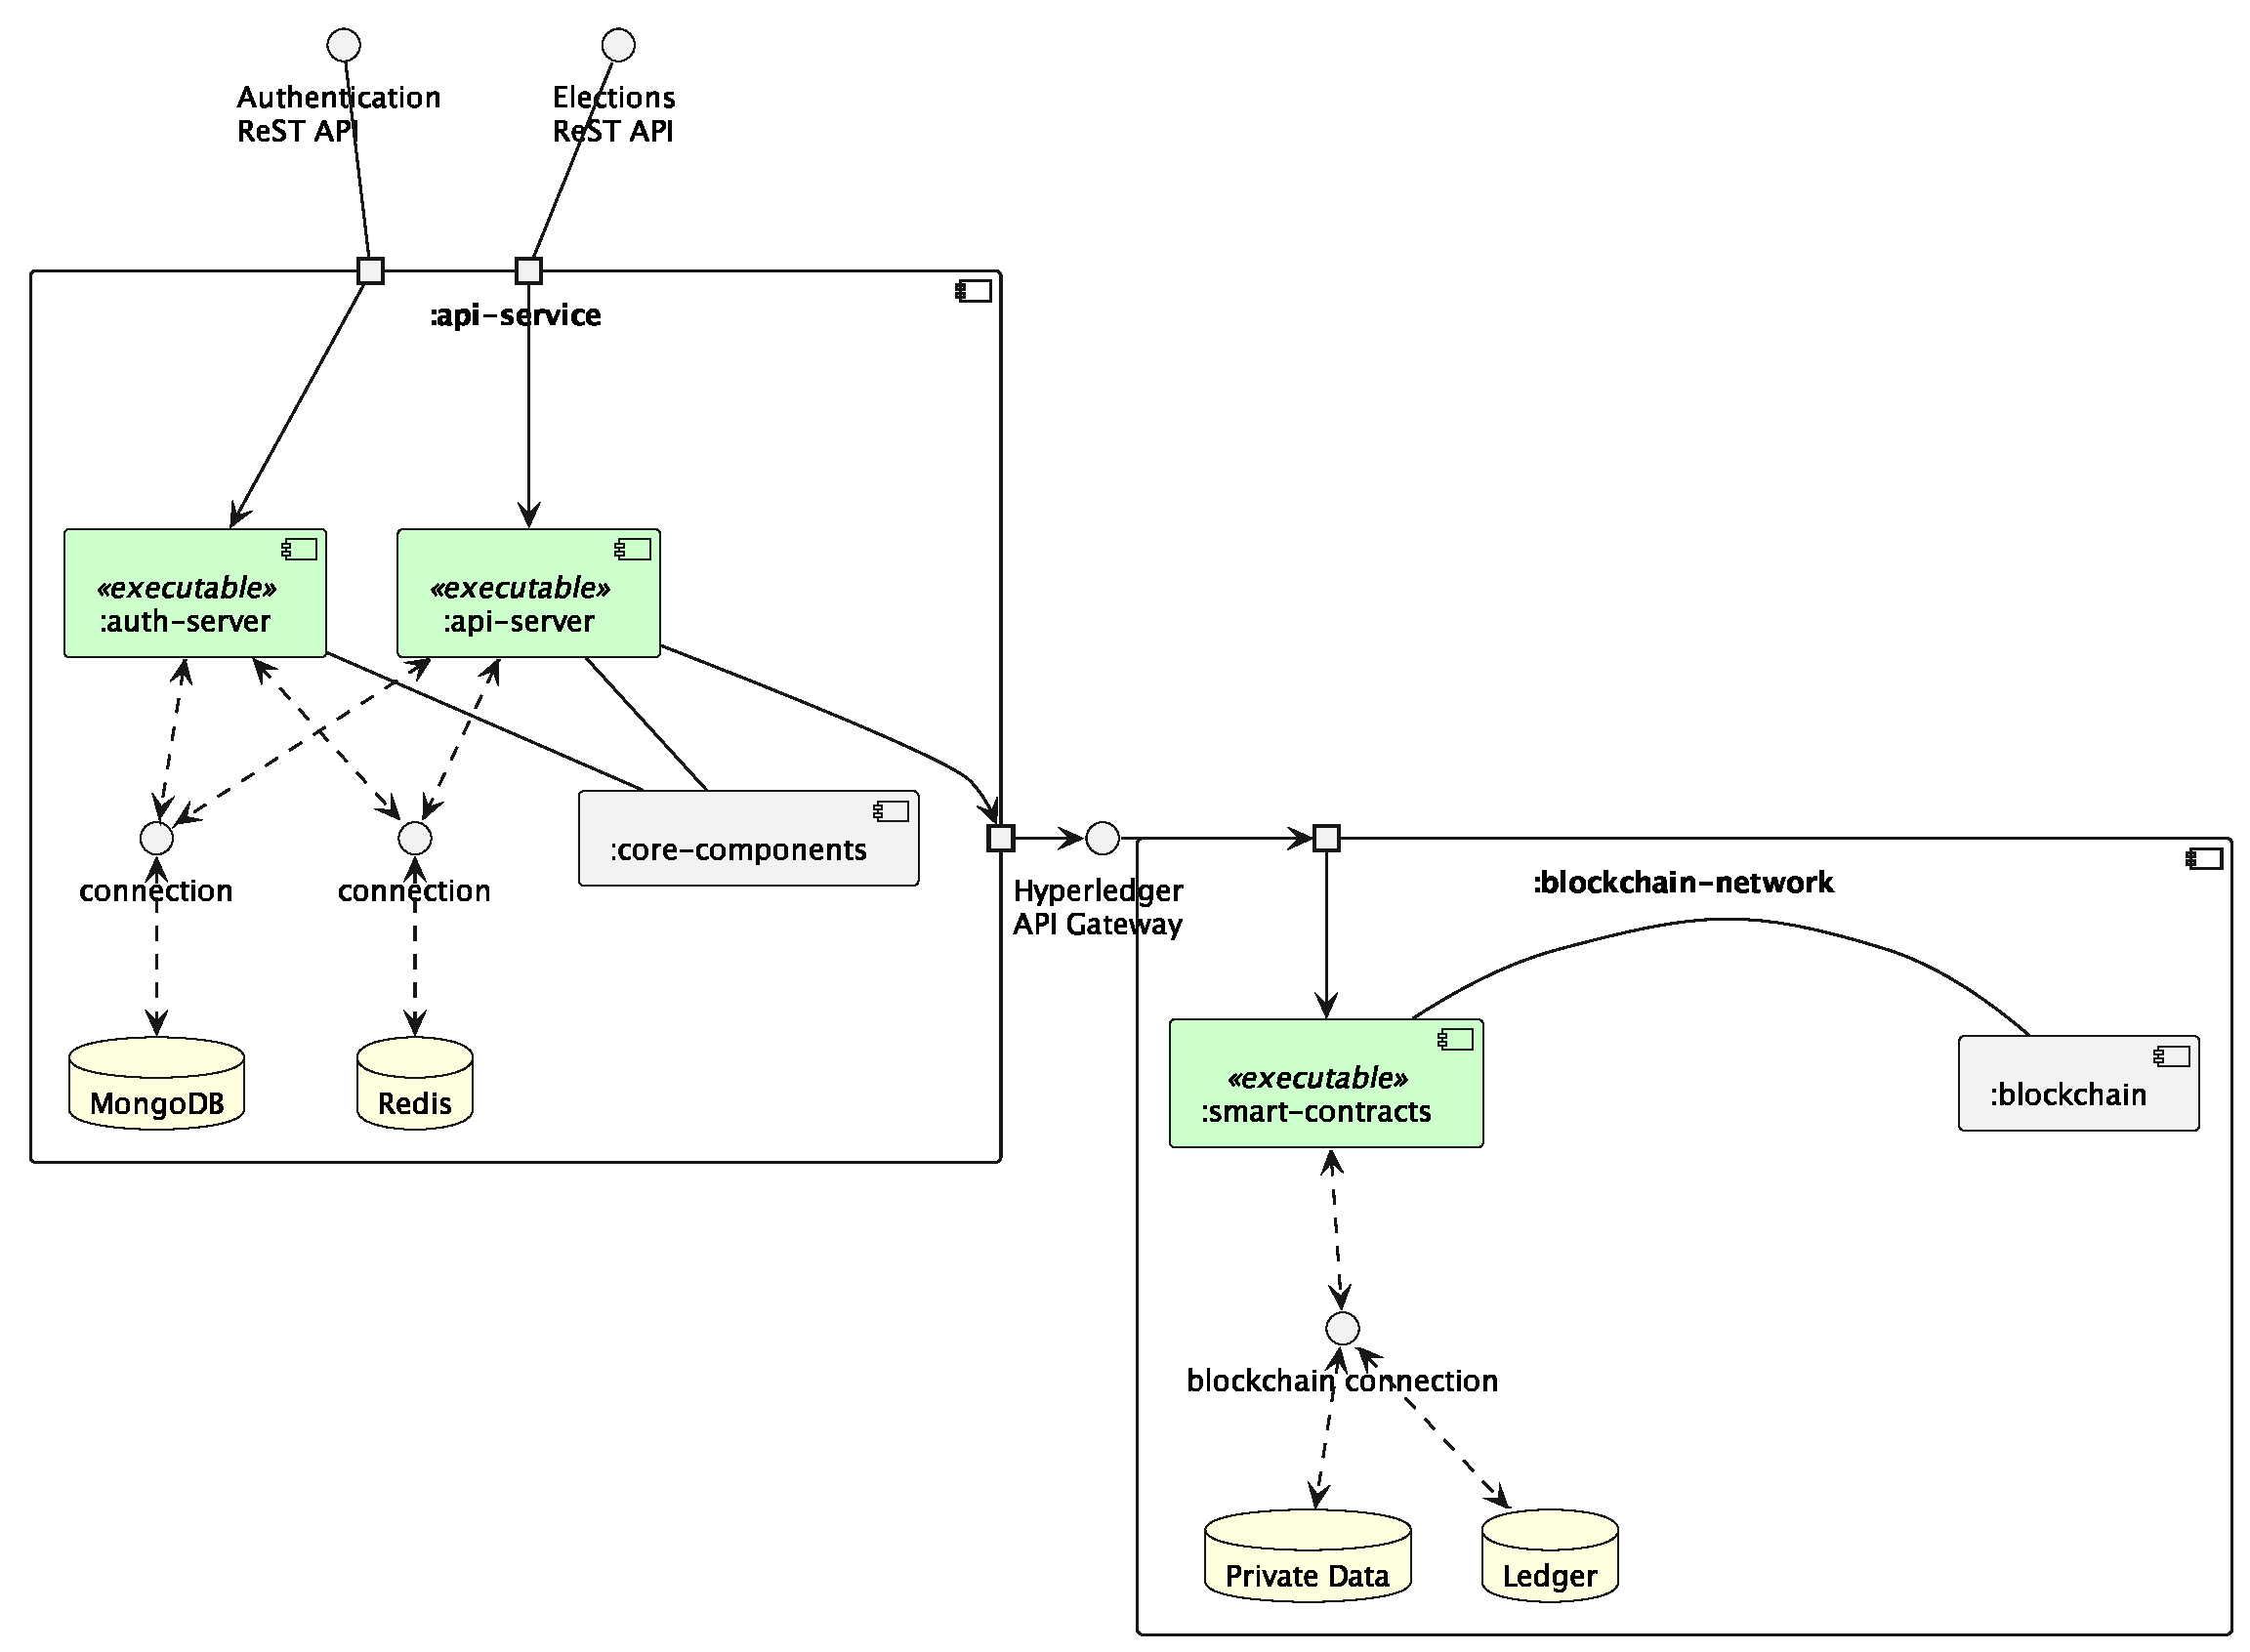
\includegraphics[width=\linewidth]{figures/system-architecture.eps}
        \caption{System architecture.}
        \label{fig:system-architecture}
    \end{figure}
\end{landscape}

Concerning the \texttt{:smart-contracts} component it consists of a JVM project with different sub-modules.
%
It's structure is presented in \Cref{fig:smart-contract-architecture}:
\begin{itemize}
    \item the \texttt{:core} submodule captures the entities and interfaces of the domain model, which are technology-independent;
    \item a \texttt{:presentation} submodule which deals with de/serializations;
    \item a \texttt{:chaincode-commons} submodule which collects all the common utility classes for the development of the Hyperledger Fabric contracts;
    \item two submodules $-$ \texttt{:chaincode-elections} and \texttt{:chaincode-votes} $-$ which contains the chaincodes managing, respectively, the elections information and the votes, and encapsulate the logic of interaction with the network and its components using the technology-dependent API abstractions (in our case the Hyperledger Fabric chaincode shim library).
\end{itemize}

\begin{figure}
    \centering
    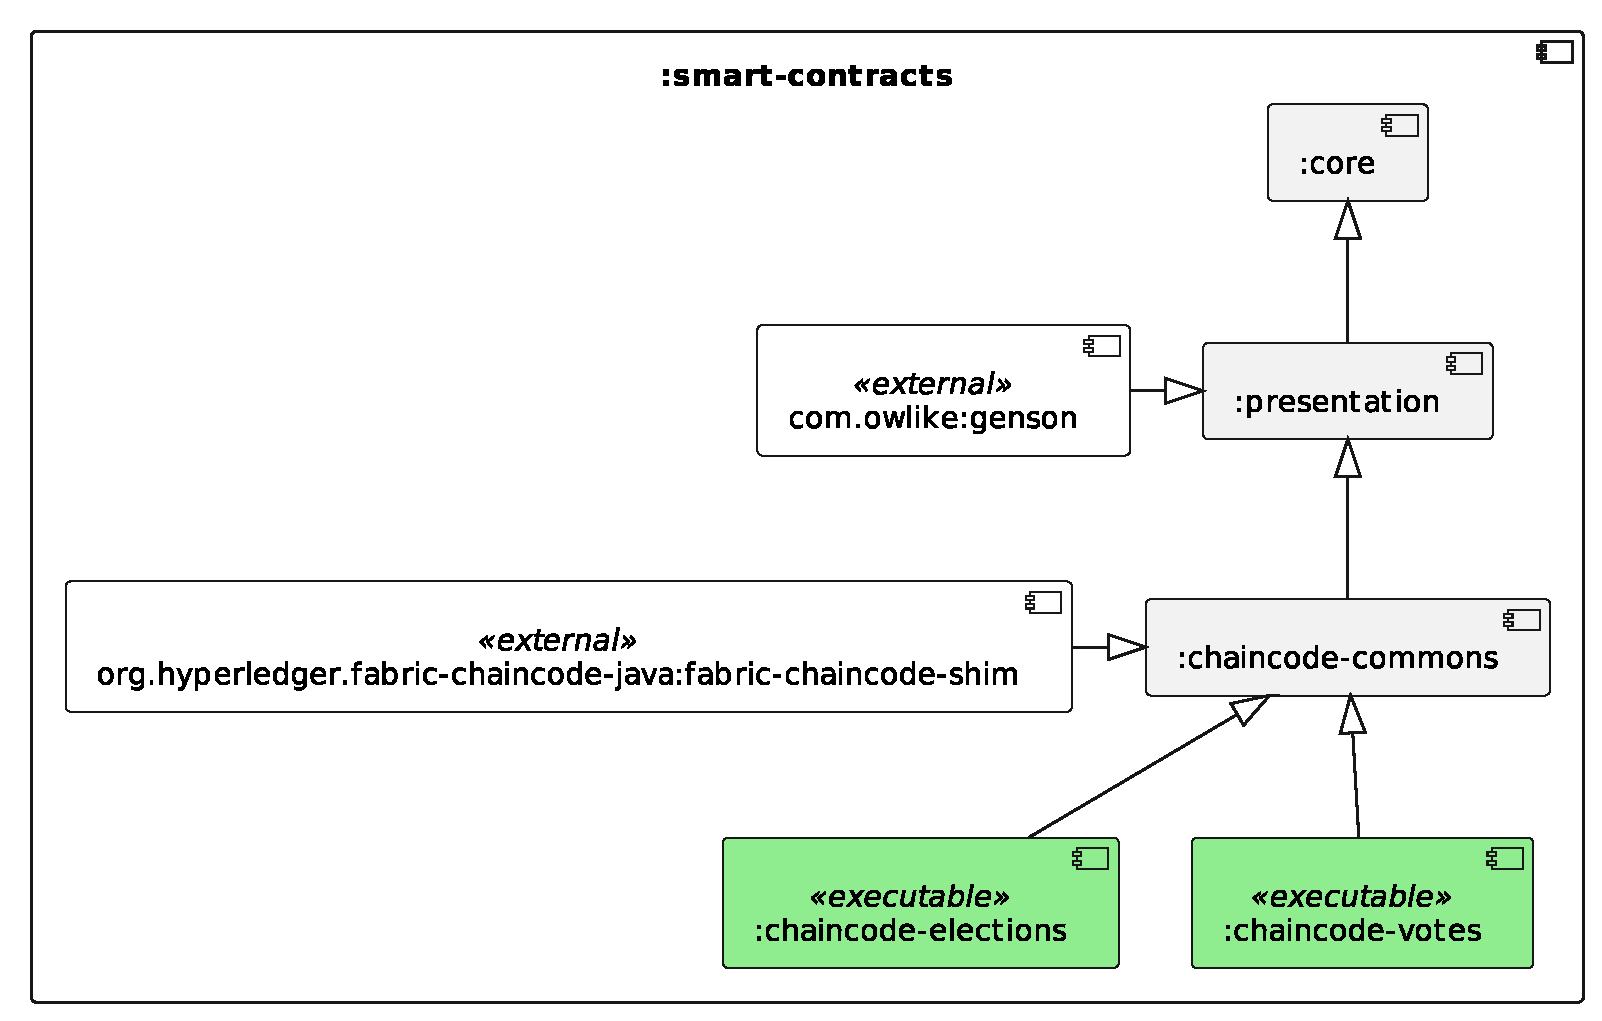
\includegraphics[width=0.85\linewidth]{figures/smart-contract-architecture.eps}
    \caption{\texttt{:smart-contracts} component architecture.}
    \label{fig:smart-contract-architecture}
\end{figure}

The internal architecture of this component decouples as much as possible the core business logic from external concerns, like technologies and used framework, making the system more maintainable and extensible: changing the technology with which to implement the blockchain in no way impacts the domain and its logic, which are assumed to remain stable over time.

The \texttt{:api-service} module exposes the core functionalities of the system through two submodules:
\begin{itemize}
    \item \texttt{:api-server} used for handling the interaction with the blockchain network and the user's management;
    \item \texttt{:auth-server} used for authentication purposes. 
\end{itemize}

We've separated the two functionalities to obtain a more modular and extensible system. Even if the authentication service stops working, the system will still be able to provide its functionality to users who are already authenticated.
%
Both \texttt{:api-server} and \texttt{:auth-server} submodules are based on the Express.js framework and share some common functions (\texttt{:common}).

Other than the blockchain the system relies on two databases:
\begin{itemize}
    \item A \texttt{MongoDB} service to store persistent information, i.e., user data and authentication tokens.
    \item A \texttt{Redis} database that is used for storing temporary data, i.e., the number of requests for a specific endpoint.
\end{itemize}

\fi
%% -------------------------------------- DS ----------------------------

\subsection{Technologies}
\label{sec:technologies}

%% -------------------------------------- DS ----------------------------
\iffalse

After evaluating different valid blockchain technologies, including Corda (R3) \cite{corda} and Tendermint \cite{tendermint}, Hyperledger Fabric has been chosen for this project for the following main reasons:

\begin{itemize}
    \item It is a general purpose \textit{permissioned} blockchain, with all the advantages described in \Cref{sec:background};
    \item It is highly configurable and customizable, like the possibility to plug different consensus mechanisms or the support of several mainstream programming languages for the smart contracts (Go, JavaScript \& TypeScript, Java \& Kotlin);
    \item It offers mechanisms that raise the bar of confidentiality and higher fine-grained control over ledger access, thanks to channels and private data collections;
    \item It has an active and growing community of developers and contributors, as well as detailed documentation.
\end{itemize}

In addition, one of the project goals is to provide a uniform API to interact with the system. 
%
To do this a ReST approach has been used, which is a widely adopted standard for exposing APIs. 
%
ReST gives different advantages:

\begin{itemize}
    \item \emph{Optimal access to the resources}: Rest requires a resource-centric design, this means that the API will be structured around the resources that are exposed. In this way, it's possible to have fine-grained control over the access and management of the resources.
    \item \emph{Stateless}: ReST API requests are stateless, which means they're independent of each other. This allows to scale the system horizontally, without having to worry about the state of the system.
    \item \emph{Expressive}: ReST APIs are expressive, this means that the APIs are designed in a way that is easy to understand and use. This allows to have a more maintainable and extensible system.
\end{itemize}

\fi
%% -------------------------------------- DS ----------------------------

\section{Implementation Details}

\subsection{API Server}

%% -------------------------------------- DS ----------------------------
\iffalse

The interesting implementation details of the project, divided by blockchain network, API and smart contracts, are presented below.

\subsection{Blockchain Network}
\label{sec:blockchain-network-impl}

This section focuses on the most important network configurations, primarily focusing on the channel ones.
%
The overall process of creation and deployment of the network and its component on top of Docker containers, as well as the CAs configurations and identities registration, is described in \Cref{deployment-details}.

The channel artifacts are generated starting from a set of YAML configuration files, which are presented hereafter.
%
All the configuration files and scripts concerning the channels can be found inside the \texttt{channels\_config} folder of the \texttt{blockchain} module.

\subsubsection*{\texttt{configtx.yaml}}

This configuration file is used to define and configure the network, including the organization's definitions, policies and other important parameters.
%
In the following are presented the most relevant sections:

\begin{itemize}
    \item \textbf{Organizations}: this section defines the different organizations that participate in the network. Each organization has a name, an ID, and specifies its cryptographic material (\texttt{MSPDir} field), as well as a set of \textbf{\textit{signature policies}}: each of them has a rule that specifies the set of organizations and identities whose signatures can satisfy the policy. In other words, they define the access control rules within an organization, governing who has permission to write, read, administer the channel and endorse (i.e. sign) a smart contract transaction. The syntax supports arbitrary combinations of \texttt{AND} and \texttt{OR}. The \texttt{org2} definition of this project's network is shown in \Cref{lst:org-definition}: for example, the \textit{Admins} policy can only be satisfied by transactions submitted by an identity with an admin role, while only identities with a peer role can satisfy the \textit{Endorsement} policy; all clients, peers and admin of both \texttt{org2} and \texttt{org3} can read, while only admin and client identities of \texttt{org2} are allowed to write.
    
    \yamlimport[
        caption={\texttt{org2} definition.},
        label={lst:org-definition},
    ]{listings/configtx-orgs.yaml}

    \item \textbf{Application}: defines the policies that govern how peer organizations can interact with application channels. In particular, here we specify \texttt{ImplicitMeta} policies, which is a Hyperledger Fabric jargon to specify that they are compositions of the simpler \textit{signature policies} defined in the \texttt{Organizations} section. All of them follow the following pattern: \texttt{<ANY|ALL|MAJORITY> <SubPolicyName>}. In our case, for channel 2, since we have chosen a \texttt{MAJORITY} application endorsement policy, both \texttt{org2} and \texttt{org3} must agree on the transaction response (see \Cref{fig:policies}): the criterion by which each organization approves is driven by its \textit{signature} endorsement policy defined above; in this case is sufficient one peer per organization approval. Therefore, for every transaction concerning channel 2 we expect one peer of each organization to be contacted, and in order to be valid, both must agree on the outcome.
    
    \yamlimport[
        caption={Application definition.},
        label={lst:app-definition}
    ]{listings/configtx-app.yaml}

    \begin{figure}
        \centering
        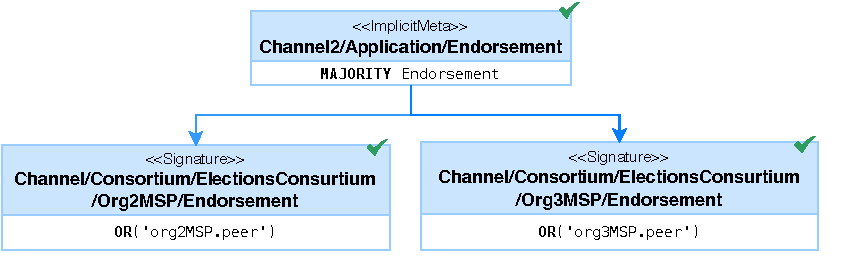
\includegraphics[width=0.95\linewidth]{figures/policies.pdf}
        \caption{Policy configuration hierarchy.}
        \label{fig:policies} 
    \end{figure}

    \item \textbf{Orderer}: This section contains configuration details for the orderer nodes, such as their addresses, consensus type, the amount of time to wait before creating a batch, the batch size, and other relevant parameters.
    Moreover, are specified the policies that, similarly to the Application section, govern the ordering nodes.
    The chosen consensus is the \texttt{etcdraft} implementation.
    
    \yamlimport[
        caption={Orderer definition.},
        label={lst:orderer-definition}
    ]{listings/configtx-orderer.yaml}

    \item \textbf{Channel}: this section defines the policies that govern the highest level of the channel configuration. In an application channel, these policies govern the hashing algorithm, the data hashing structure used to create new blocks, and the channel capability level. Default policies are provided by Hyperledger Fabric which, in most cases, there is no need to change.
    
    \yamlimport[
        caption={Channels definition.},
        label={last:channels-definition}
    ]{listings/configtx-channel.yaml}

    \item \textbf{Profiles}: The \texttt{configtxgen} tool reads this section to build a channel configuration. Each profile uses YAML syntax to gather data from other sections of the file.
\end{itemize}

\subsubsection*{\texttt{core.yaml} and \texttt{orderer.yaml}}

These files are used to configure settings for the core components of, respectively, a peer node and an orderer node. 

Among the plethora of options that can be configured the focus is on the following:
\begin{itemize}
    \item peer connectivity information, like identifier, network identifier, the address at local network interface the peer will listen on and gossip configurations;
    \item \texttt{tls} is enabled;
    \item ledger world state database has been set to CouchDB for the reasons already discussed in \Cref{sec:background-ledger}.
\end{itemize}

Note that, for this project, a single \texttt{core.yaml} and \texttt{orderer.yaml} files have been configured with common configurations for all the peers and orderers.
%
The options intrinsically related to peer and orderers instances, like the address, will be overridden during the creation of the network with environment variables.
%
This guarantees to have a single template for all the peers with static configuration while configuring dynamic ones at channel creation time with scripts.

\subsection{Smart Contracts}

Hyperledger Fabric smart contracts are implemented through classes annotated with \texttt{@Contract} implementing the chaincode-shim \texttt{ContractInterface}, while transactions are simple methods labelled with \texttt{@Transaction(intent = ...)} where the \texttt{intent} specifies the semantics for the transaction:
\begin{itemize}
    \item \texttt{Transaction.TYPE.SUBMIT} indicates that this function is intended to be called with the \textit{submit} semantics, i.e. the transaction will update the ledger and modify the state of the blockchain, producing a lasting impact on the network's ledger;
    \item \texttt{Transaction.TYPE.EVALUATE} indicates that this is intended to be called with the \textit{evaluate} semantics, i.e. the transaction is read-only and should not make any updates to the ledger. It is primarily used for querying the blockchain to retrieve information or perform calculations without affecting the ledger's state.
\end{itemize}

The general structure of a smart contract is presented in \Cref{lst:smart-contract}.

\javaimport[
    caption={General structure of a Hyperledger Fabric smart contract},
    label={lst:smart-contract}
]{listings/HFSmartContract.java}

A few things to notice:

\begin{itemize}
    \item inside the \texttt{@Contract} annotation is possible to specify a custom \texttt{SerializerInterface} which will be used to (un)marshall transaction inputs;
    \item every transaction receives a transaction context, which Hyperledger Fabric automatically provides when a smart contract is invoked. This context includes both system and user elements, enabling smart contract developers to interact with the ledger and store or retrieve user-defined data across consecutive transaction calls. An overview of the main functionalities offered by the chaincode-shim library is described in the UML class diagram shown in \Cref{fig:chaincode-api}.
\end{itemize}

\begin{figure}
    \centering
    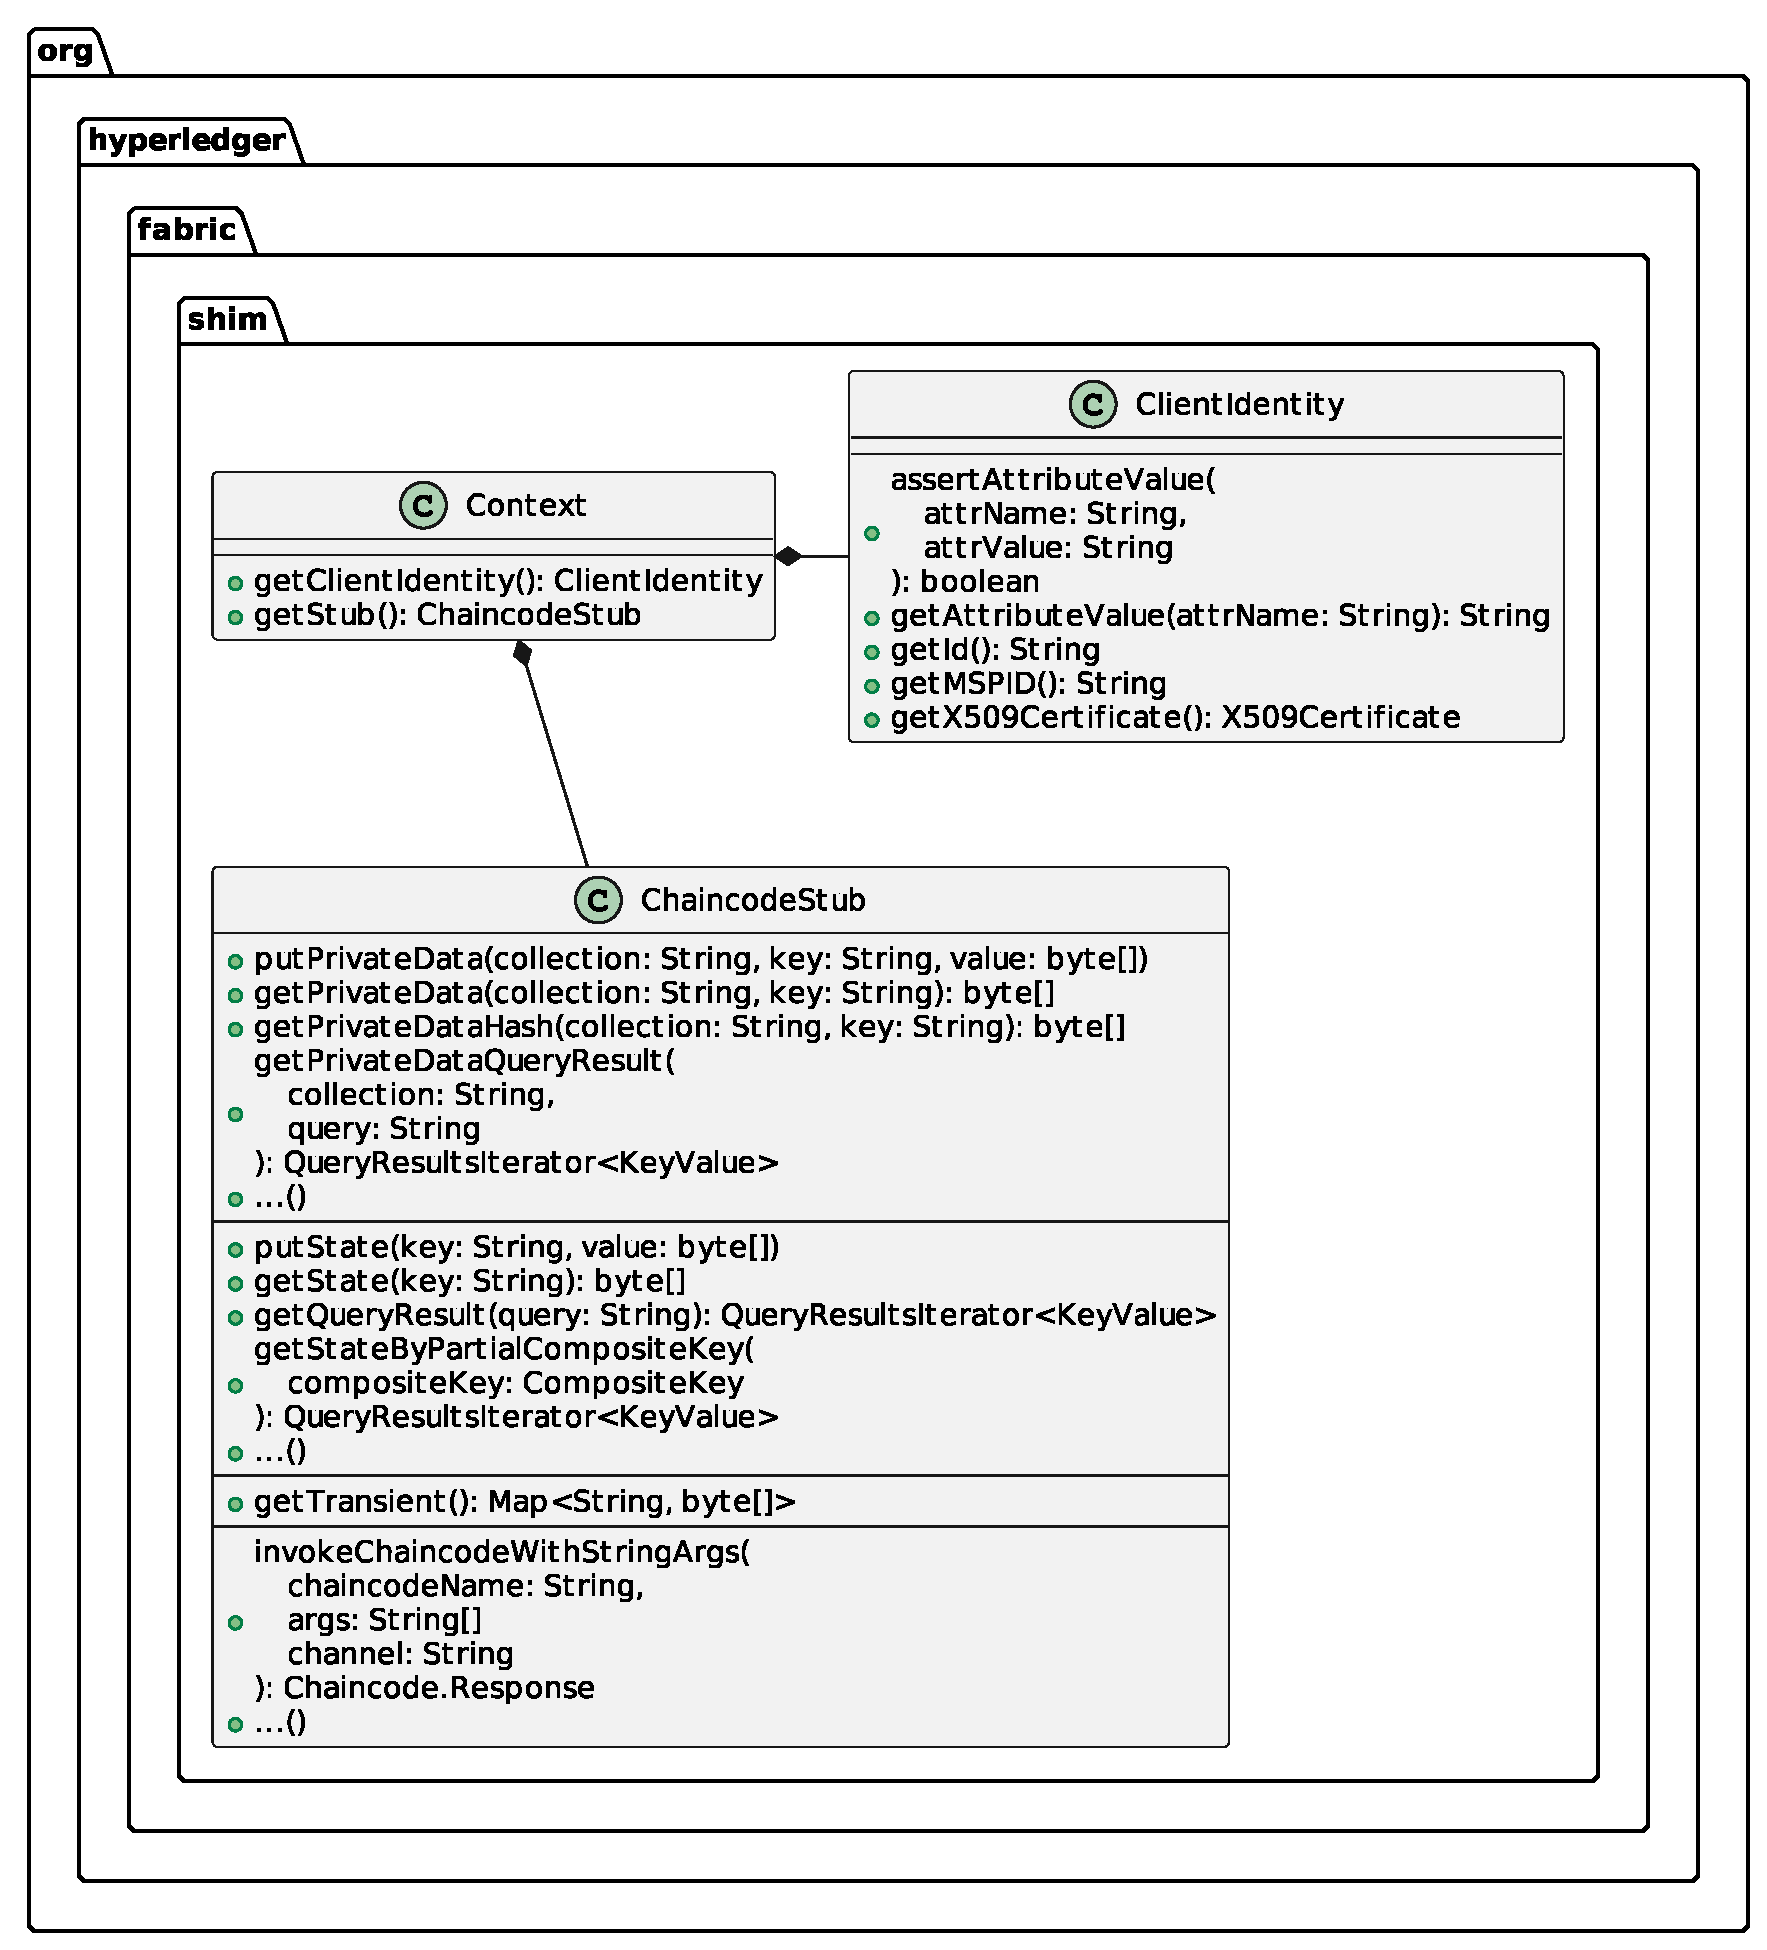
\includegraphics[width=\linewidth]{figures/chaincode-shim-api.eps}
    \caption{Overview of the main functions offered by the chaincode-shim API to interact with the ledger.}
    \label{fig:chaincode-api} 
\end{figure}

Other important points to highlight are how the one-time codes are generated, where they are saved and the mechanism used for hiding the transaction inputs. 

As stated in \Cref{sec:non-functional-requirements} for the generation of codes a deterministic algorithm has been used, hashing the static information of the election with a randomly generated seed passed to the blockchain by the API server.
%
We assume the API server is a trustworthy component that is impossible to tamper with.

Codes are then stored inside \textbf{Private Data} collections.
%
This ensures that only organization 2, the one in charge of the creation of codes, has a copy and can access the private collection where they are stored.

From an implementation point of view accessing a private data collection is almost the same as accessing the world state: this implies that private data collections are merely an implementation detail that is completely transparent to the client application.

\javaimport[
    caption={Examples of how to retrieve and store data on a private collection},
    label={lst:pvd}
]{listings/PrivateData.java}

Private data collections can be configurable in terms of endorsement policy, time to live (in terms of the number of blocks), access control and information dissemination through a JSON configuration file (see \\ \texttt{smart-contracts/chaincode-votes/src/main/resources/collections-config.json}).
%
In particular:
\begin{itemize}
    \item \texttt{policy} defines the organization peers allowed to persist the collection data;
    \item \texttt{requiredPeerCount} defines the minimum number of peers that must receive and store the private data in order for an endorsement to be considered valid;
    \item \texttt{maxPeerCount} the number of other peers that the current endorsing peer will attempt to distribute the data to.
    \item \texttt{blockToLive} represents how long the data should live on the private database in terms of blocks. To keep indefinitely set to 0;
    \item \texttt{memberOnlyRead} is a boolean value indicating that  only clients belonging to one of the collection member organizations have read access to private data;
    \item \texttt{memberOnlyWrite} a boolean value indicating that only clients belonging to one of the collection member organizations have write access to private data;
    \item \texttt{endorsementPolicy} defines the endorsement policy that needs to be met in order to write to the private data collection.
\end{itemize}

\jsonimport[
 	caption={Private code collection configuration},
 	label={lst:pvd-codes},
]{listings/collections-config.json}

Until now we have discussed how to store data in private collections but we have not yet considered a potential vulnerability: Hyperledger Fabric records the submitter's digitally signed transaction inputs, as well as the digitally signed transaction responses.
%
Therefore, if not protected in some way, the user and related one-time codes are available for all to see, as they are recorded in the transaction distributed to the network.
%
In order to avoid this issue Hyperledger Fabric offers a mechanism, called \textbf{transient data}, whereby the transaction inputs are not recorded anymore.
%
When a client initiates a transaction, it can attach transient data to the transaction proposal: the chaincode-shim API, as well as the Gateway one, exposes methods allowing the retrieving and packing of data inside transient maps (\Cref{fig:chaincode-api}).
%
This data is then endorsed by the required peers and included in the transaction payload during the ordering process. 
%
However, unlike the actual transaction data, transient data is not recorded on the blockchain ledger and is not visible to other nodes in the network.

Therefore, transient data have been used to hide the associations between code and user, as well as, expressed choice and code. 

Due to the blockchain architecture choice of decoupling election information, the application requires a way to access static information in the chaincode that manages the votes. To achieve this, an example of cross-chaincode invocation is provided in \Cref{lst:cross-invocation}.

\javaimport[
    caption={General structure of a Hyperledger Fabric invocation of a method located in a different chaincode},
    label={lst:cross-invocation}
]{listings/CrossInvocation.java}

\begin{info}[\textit{Documentation}]
    Here are listed the links where you can find the JavaDoc of the \texttt{:smart-contracts} module:
    \begin{itemize}
        \item \href{https://tassiluca.github.io/ChainVote/smart-contracts/javadoc/chaincode-elections/}{\texttt{:chaincode-elections} API}
        \item \href{https://tassiluca.github.io/ChainVote/smart-contracts/javadoc/chaincode-votes/}{\texttt{:chaincode-votes} API}
    \end{itemize}
    (\href{https://tassiluca.github.io/ChainVote/smart-contracts/javadoc/core/}{\texttt{:core}} and \href{https://tassiluca.github.io/ChainVote/smart-contracts/javadoc/presentation/}{\texttt{:presentation}} submodules' APIs are here reported for completeness although not necessary for the ReST API service client.)
\end{info}

\subsection{Gateway}
To interact with the blockchain network, starting from version 2.4, the Hyperledger Fabric peers expose a new gRPC service, called \texttt{Gateway}, which API allows to submit transactions to the network and retrieve data from the ledger.
% 
To connect to the blockchain with the Gateway service we need to establish a new gRPC session, select a channel and a smart contract we want to invoke. The \texttt{Communicator} class was developed to simplify the overall configuration process (\Cref{fig:communicator-api}).

\begin{figure}
    \centering
    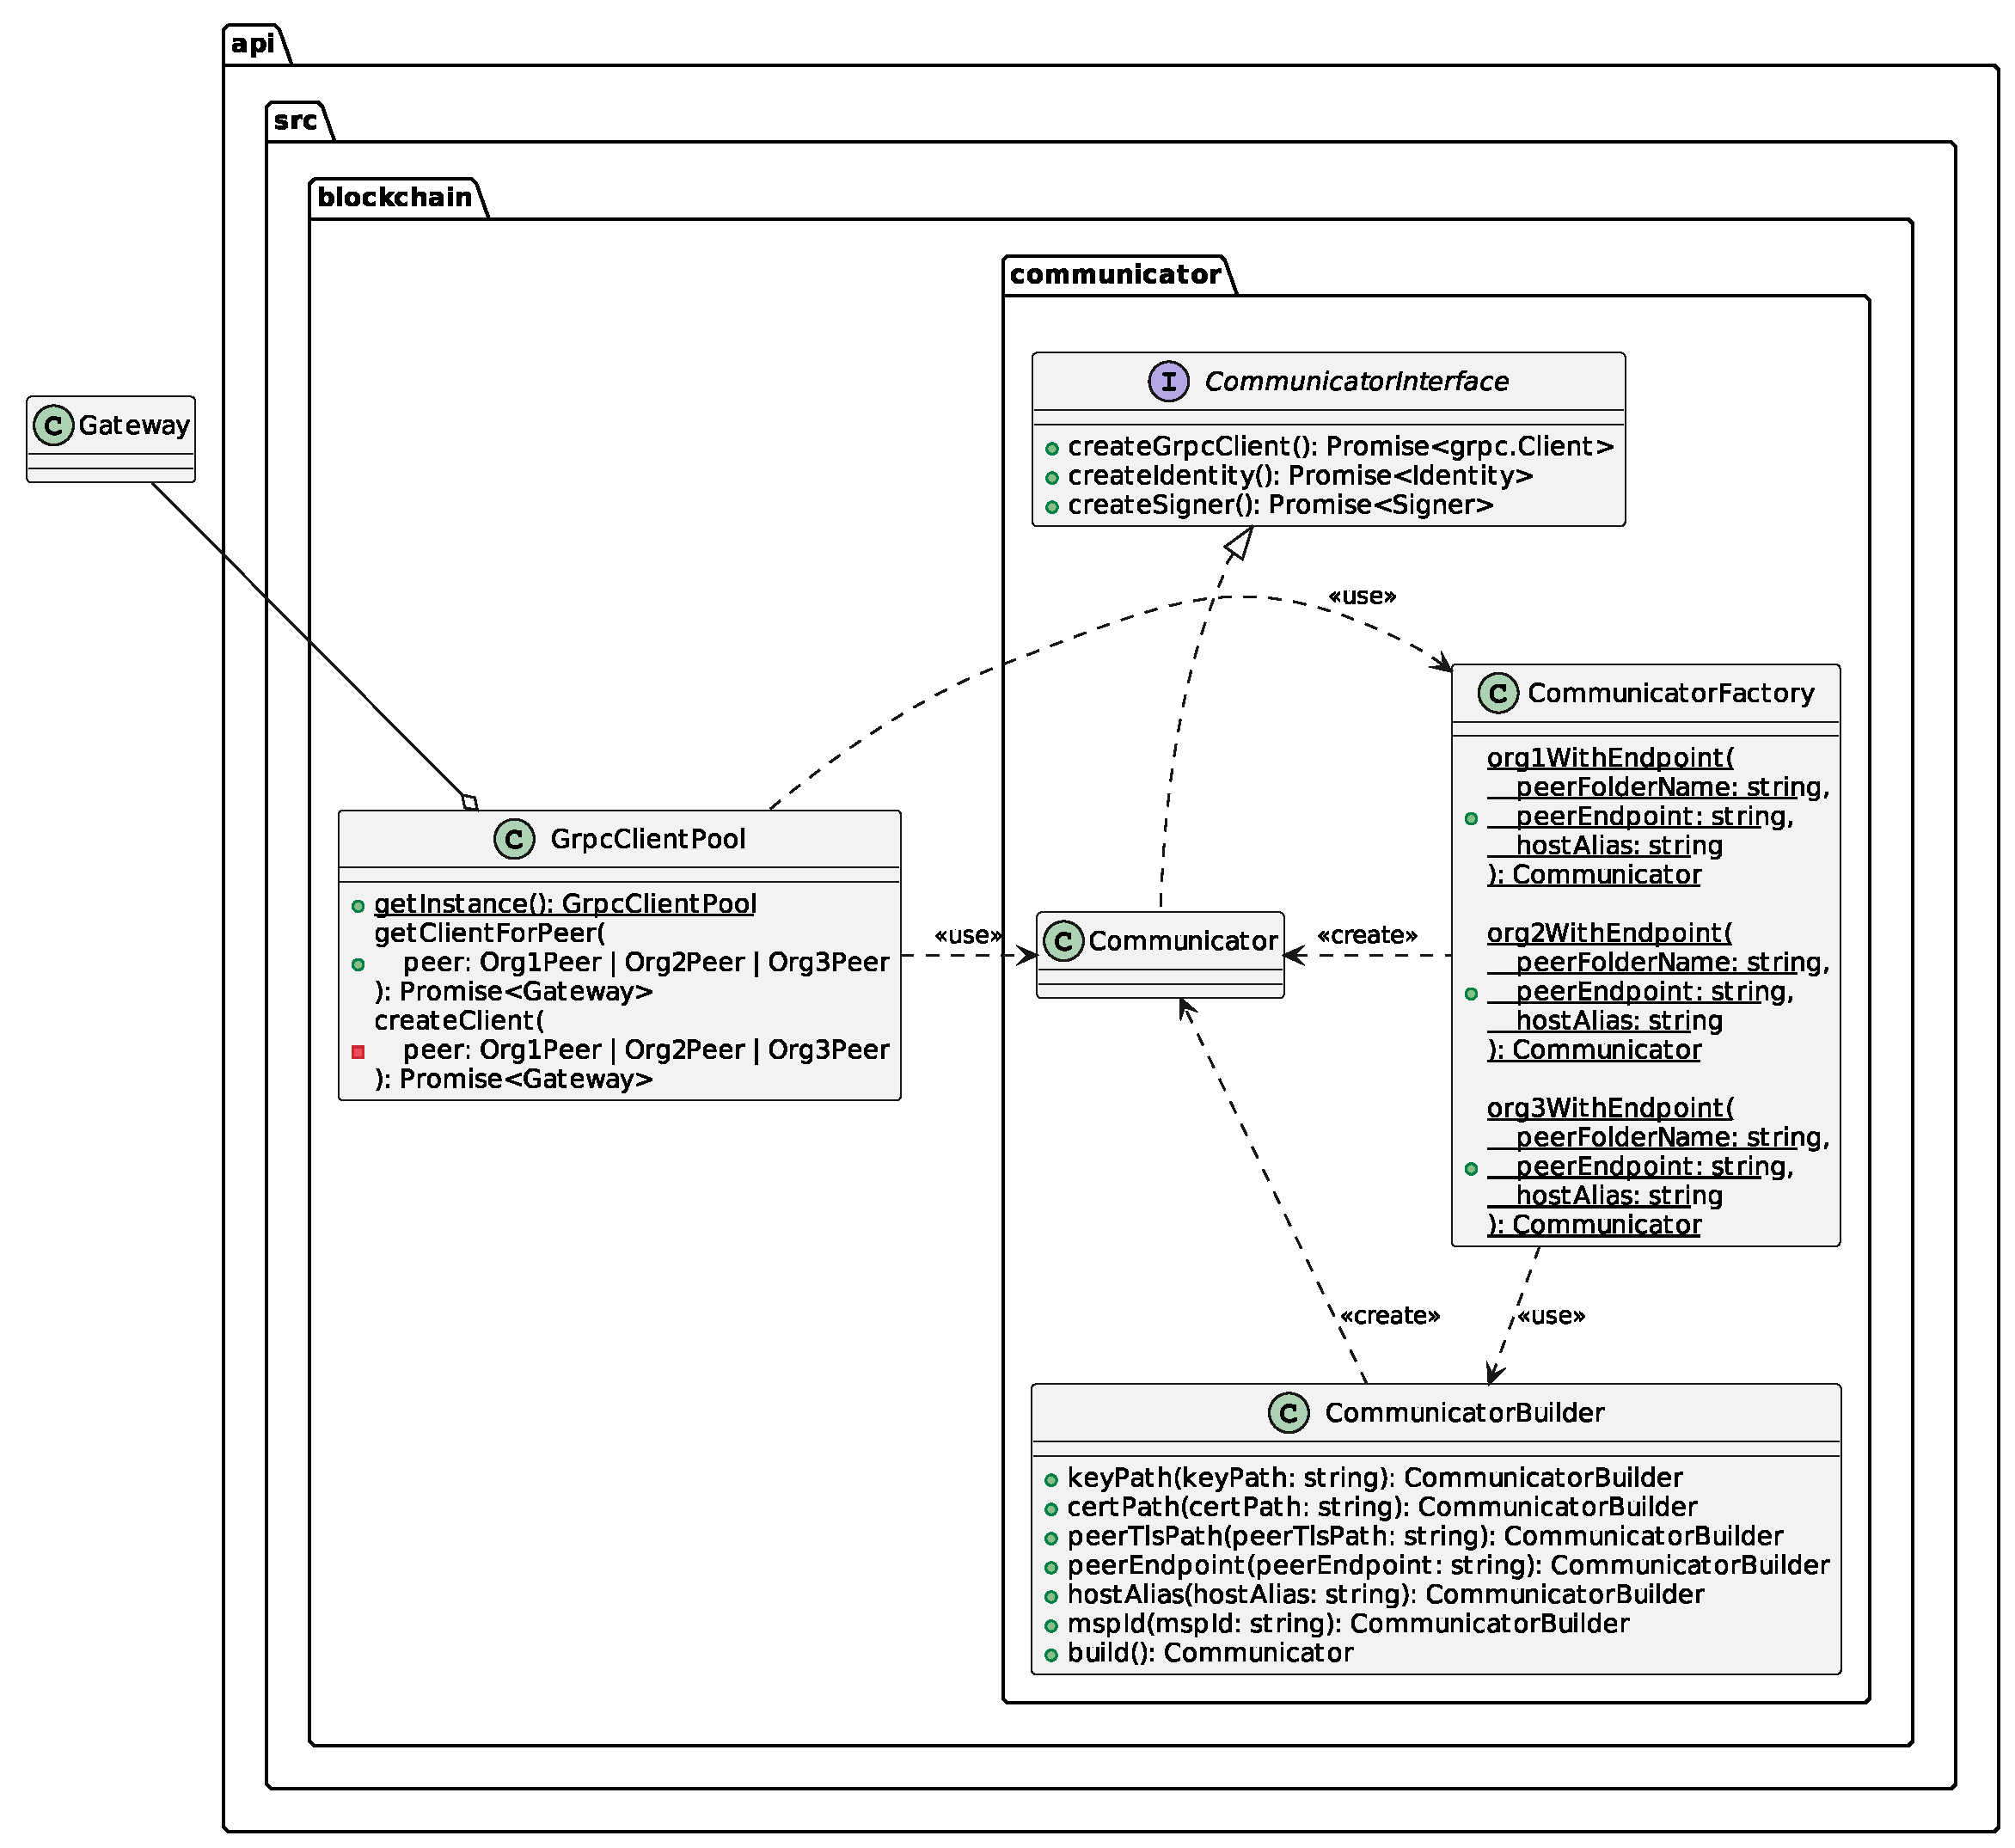
\includegraphics[width=\linewidth]{figures/communicator-api.eps}
    \caption{The communicator API component that allows the connection to the Gateway service configuration.}
    \label{fig:communicator-api} 
\end{figure}

\texttt{CommunicatorInterface} define three methods:
\begin{itemize}
    \item \texttt{createGrpcClients} establishes a new gRPC session with the peer;
    \item \texttt{createIdentity} creates an \texttt{Identity} object that represents the identity that will interact with the blockchain; for doing this it will use the certificates created by the CA during the creation of the network;
    \item \texttt{createSigner} creates a \texttt{Signer} object representing the signer of the transactions.
\end{itemize} 

The Communicator class requires several arguments for the instantiation, and this could represent a usage problem, for this purpose the \texttt{CommunicatorBuilder} and \\ \texttt{CommunicatorFactory} were developed. The first one is a builder that allows the construction of a Communicator object in a more readable way, while the latter is a factory class that creates instances of Communicator that will connect to a target peer that will act as a gateway endpoint. Since the functions exposed by the endpoints of the API server need to use a gRPC session every time they are invoked, to make the creation process less burdensome we delegate the instantiation and management of the gRPC clients to the class \texttt{GrpcClientPool}.

\jsimport[
    caption={An example of an API method that communicates with the blockchain network},
    label={lst:gateway-usage}
]{listings/create.elections.ts}

The first time that we request a client for a specific endpoint the GrpcClientPool will create a new gRPC session and will store it in a map, associating it with the endpoint. The next time that we request a client for the same endpoint, the GrpcClientPool will return the client that was created previously. This will allow us to reuse the same gRPC session for multiple requests, without having to create a new one.

\subsection{Authentication}
Authentication within the system is implemented by the use of \texttt{JWT tokens}. JWT \cite{jwt} is an open standard that allows the secure transmission of information between two parties as a JSON object. The information passed is digitally signed using the RS256 algorithm so it can be trusted and verified by an entity that requests it. Both the sign and verify functions for an access token are distributed to the \texttt{API} and \texttt{AUTH} server inside the \texttt{:common} package.

As mentioned in \Cref{uc:auth-to-the-system}, when a user tries to log in, the \texttt{AUTH} server will sign an access and a refresh token. The first one has a validity of 15 minutes while the latter one of 30, both will be securely signed by a private key and then sent back to the client. 

\jsimport[
    caption={The login method in the auth server},
    label={lst:login-auth-server}
]{listings/login.ts}

The client is responsible for securely storing the tokens and for sending them to the request that requires authentication. Before accessing the routes, \texttt{API} server verifies the validity of the access token and extract 
the information that it needs from it.
This operation is performed by a middleware that is executed before the request is processed by the route handler. It verifies the validity of the token and extracts the information that it needs from it. If the token is valid, the middleware registers the user information and sends it to the function that handles the request. If the token is not valid, the middleware sends back an error response.

\jsimport[
    caption={The middleware that handles the authentication},
    label={lst:auth-middleware}
]{listings/authentication.handler.ts}

\begin{figure}
    \centering
    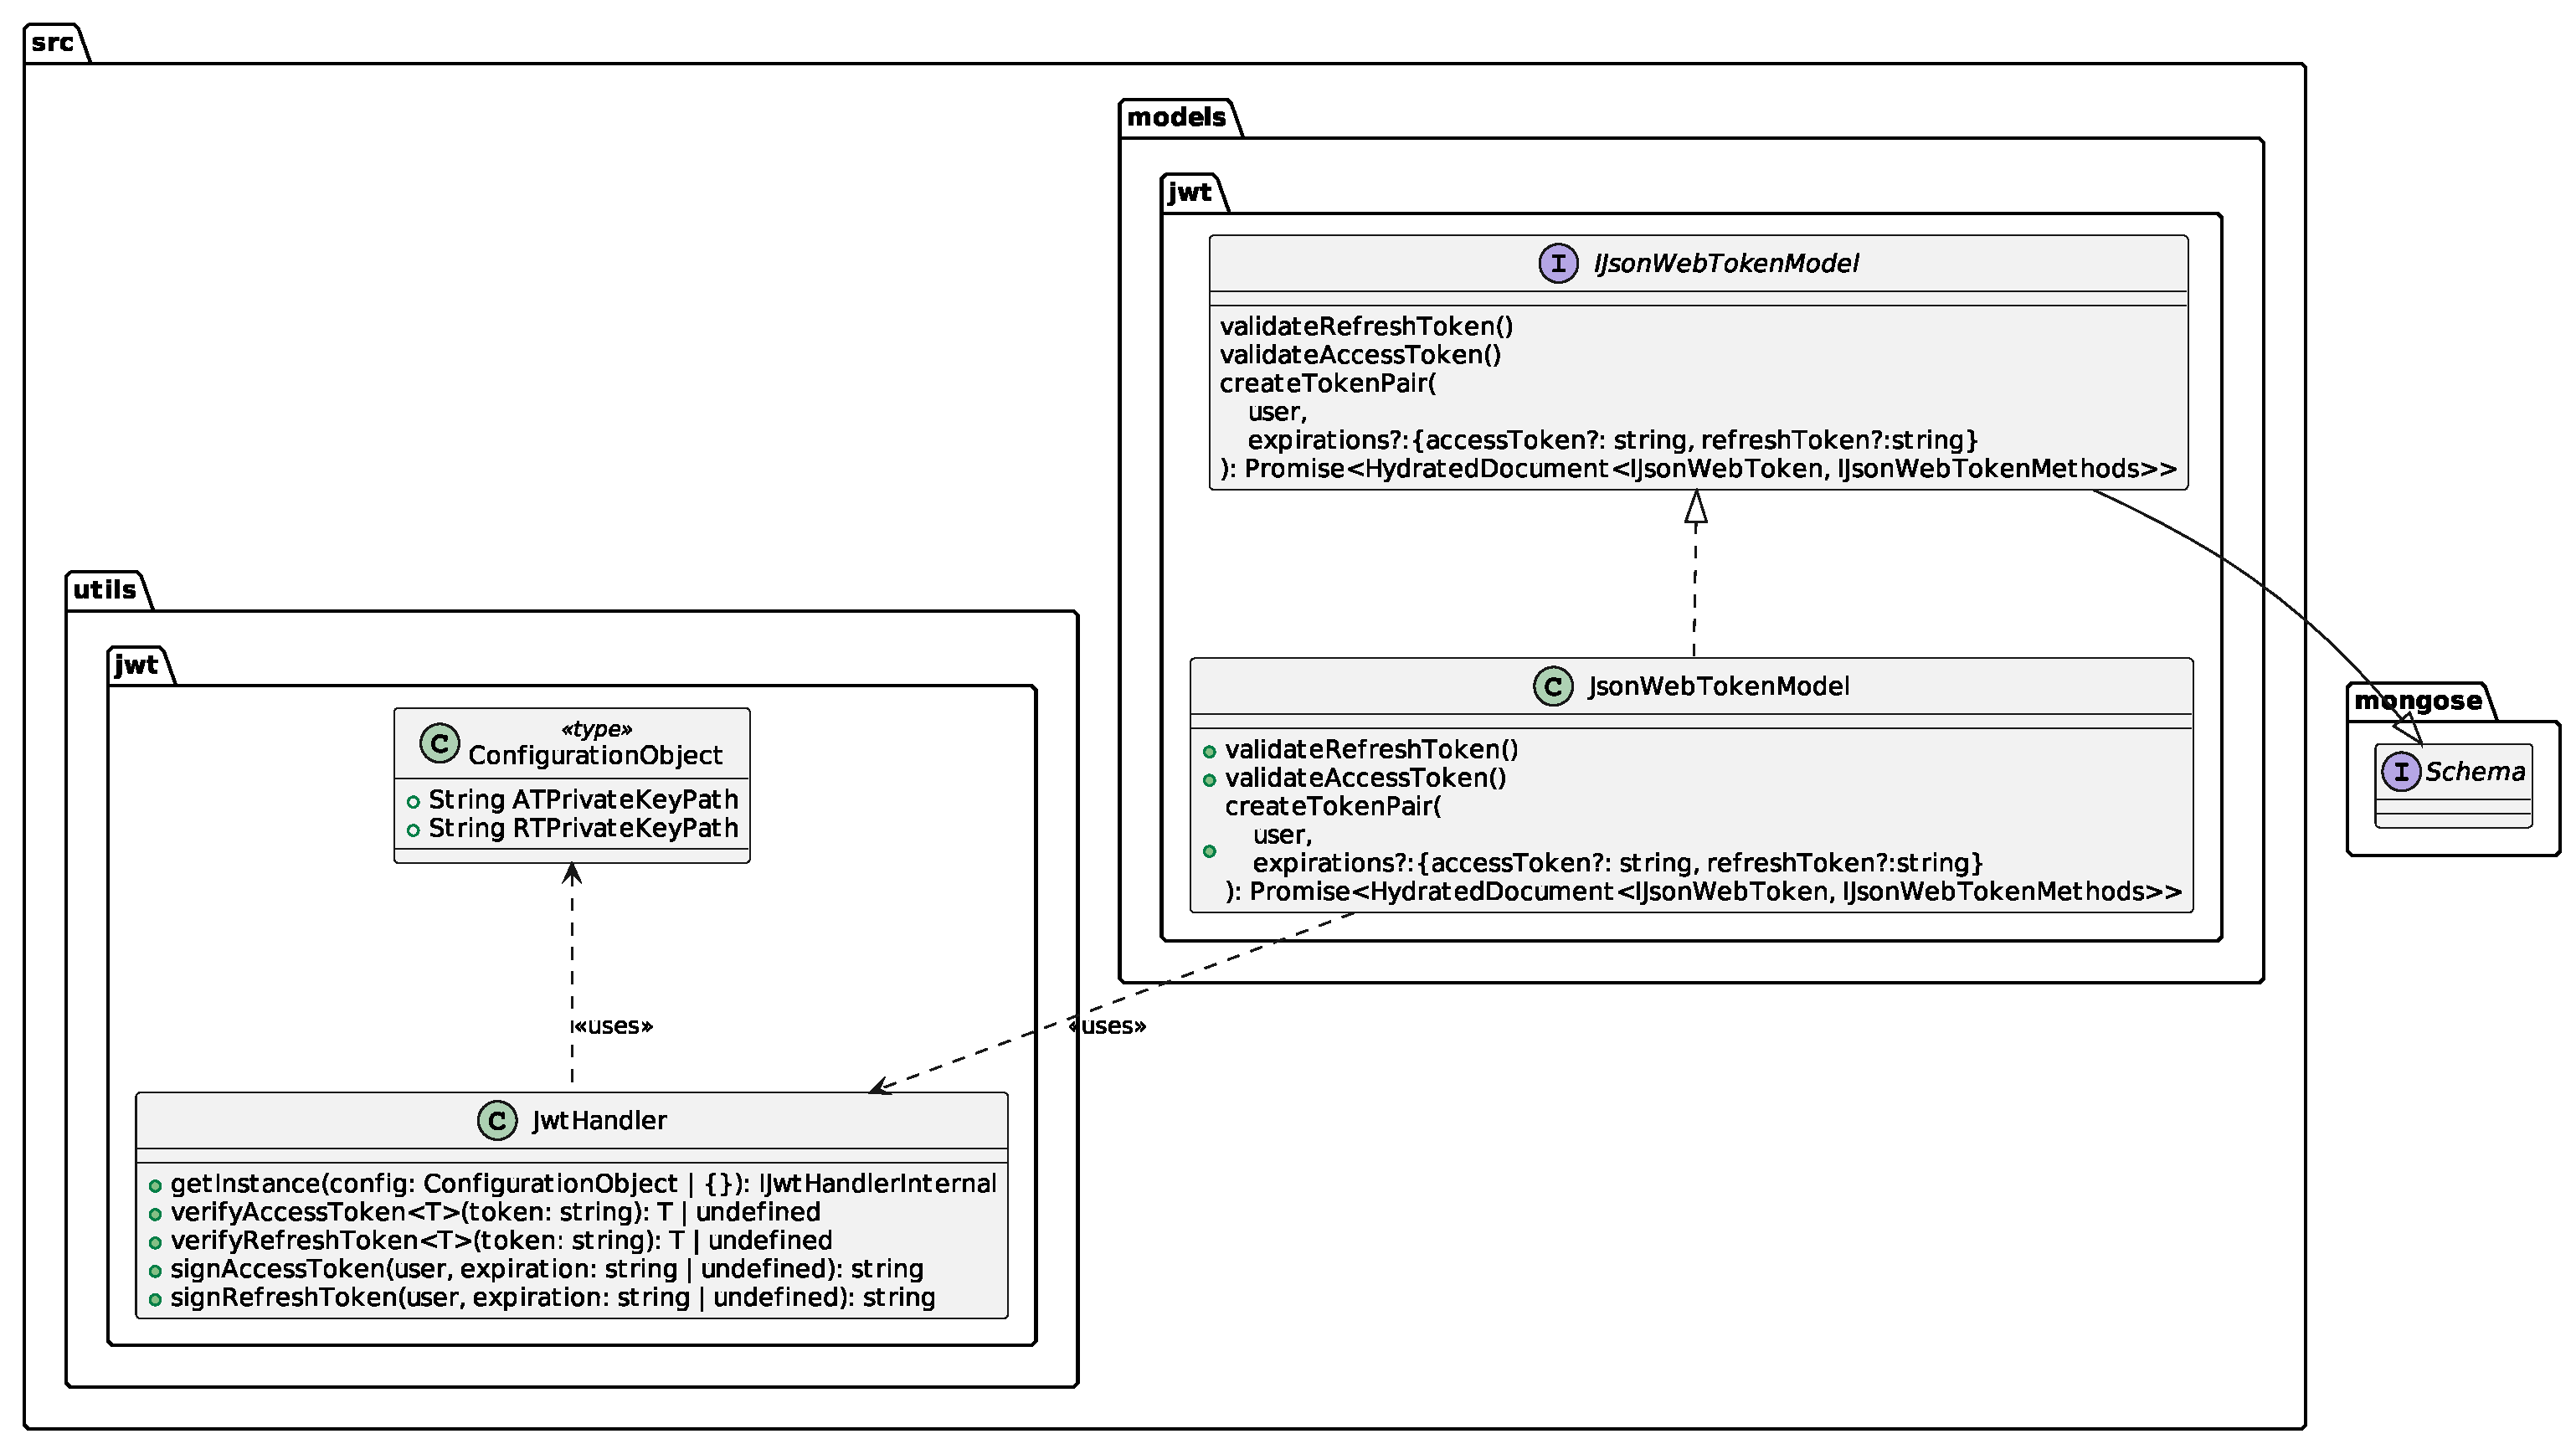
\includegraphics[width=\linewidth]{figures/jwt-api.eps}
    \label{fig:jwt-packages-api} 
    \caption{The overall API for the management of the JWT tokens}
\end{figure}

The \texttt{Jwt} model handles the verification and persistence of tokens inside the \texttt{MongoDB} database. It uses the namesake utility class, located within the \texttt{utils.jwt} package which is responsible for managing the construction of the various parts of the token.

\begin{warn}[\textit{Warning}]
    Once the network is deployed, the script copies a pair of public \& private keys in \texttt{api}, \texttt{auth} and \texttt{common} modules. While this operation simplifies the deployment process, and its testing, we're aware that in a real scenario, this would be a security issue and the private key should be stored and distributed more securely way.
\end{warn}

\subsection{Rate limiter}
We've implemented a custom rate-limiter module inside the API layer, which is responsible for limiting the number of requests that a client can send to a specific endpoint. This is done by using a \texttt{Redis} database that stores the number of requests that a client has sent to a specific endpoint. The rate limiter is implemented as a middleware that is executed before the request is processed by the route handler. It checks if the client has exceeded the maximum number of requests allowed, if so it sends back an error response to the client, otherwise, it increments the number of requests and sends the request to the route handler.

The way it works is as follows: each controller specifies a set of rules for each endpoint that can vary from the type of request.

\jsimport[
    caption={The definitions of the rules for the rate-limiter},
    label={lst:rate-limiter-rules}
]{listings/api.rule.ts}

In \Cref{lst:rate-limiter-rules} we specified the rules for three endpoints, each of them specify for the \texttt{verb} type two parameters:
\begin{itemize}
    \item \texttt{time}: The time window in which the requests are counted.
    \item \texttt{limit}: The maximum number of requests that can be sent in the specified time window.
\end{itemize}

So, for example, \texttt{endpoint\_name\_1} can receive a maximum of 50 requests in 18 seconds if the request type is \texttt{POST} and 60 requests in 14 seconds if the request type is \texttt{GET}.
The set of rules is then passed to the RateLimiter middleware which retrieves the IP address of the client and the endpoint that is being requested. 
Route checking is done on data saved on a \texttt{Redis} database. To make this solution more modular and extensible a Storage (\texttt{ApiLimiterStorage}) interface was devised that defines the operations to be performed on the data. 

\jsimport[
    caption={The limiter middleware},
    label={lst:rate-limiter-middleware}
]{listings/api.limiter.ts}

\begin{figure}
    \centering
    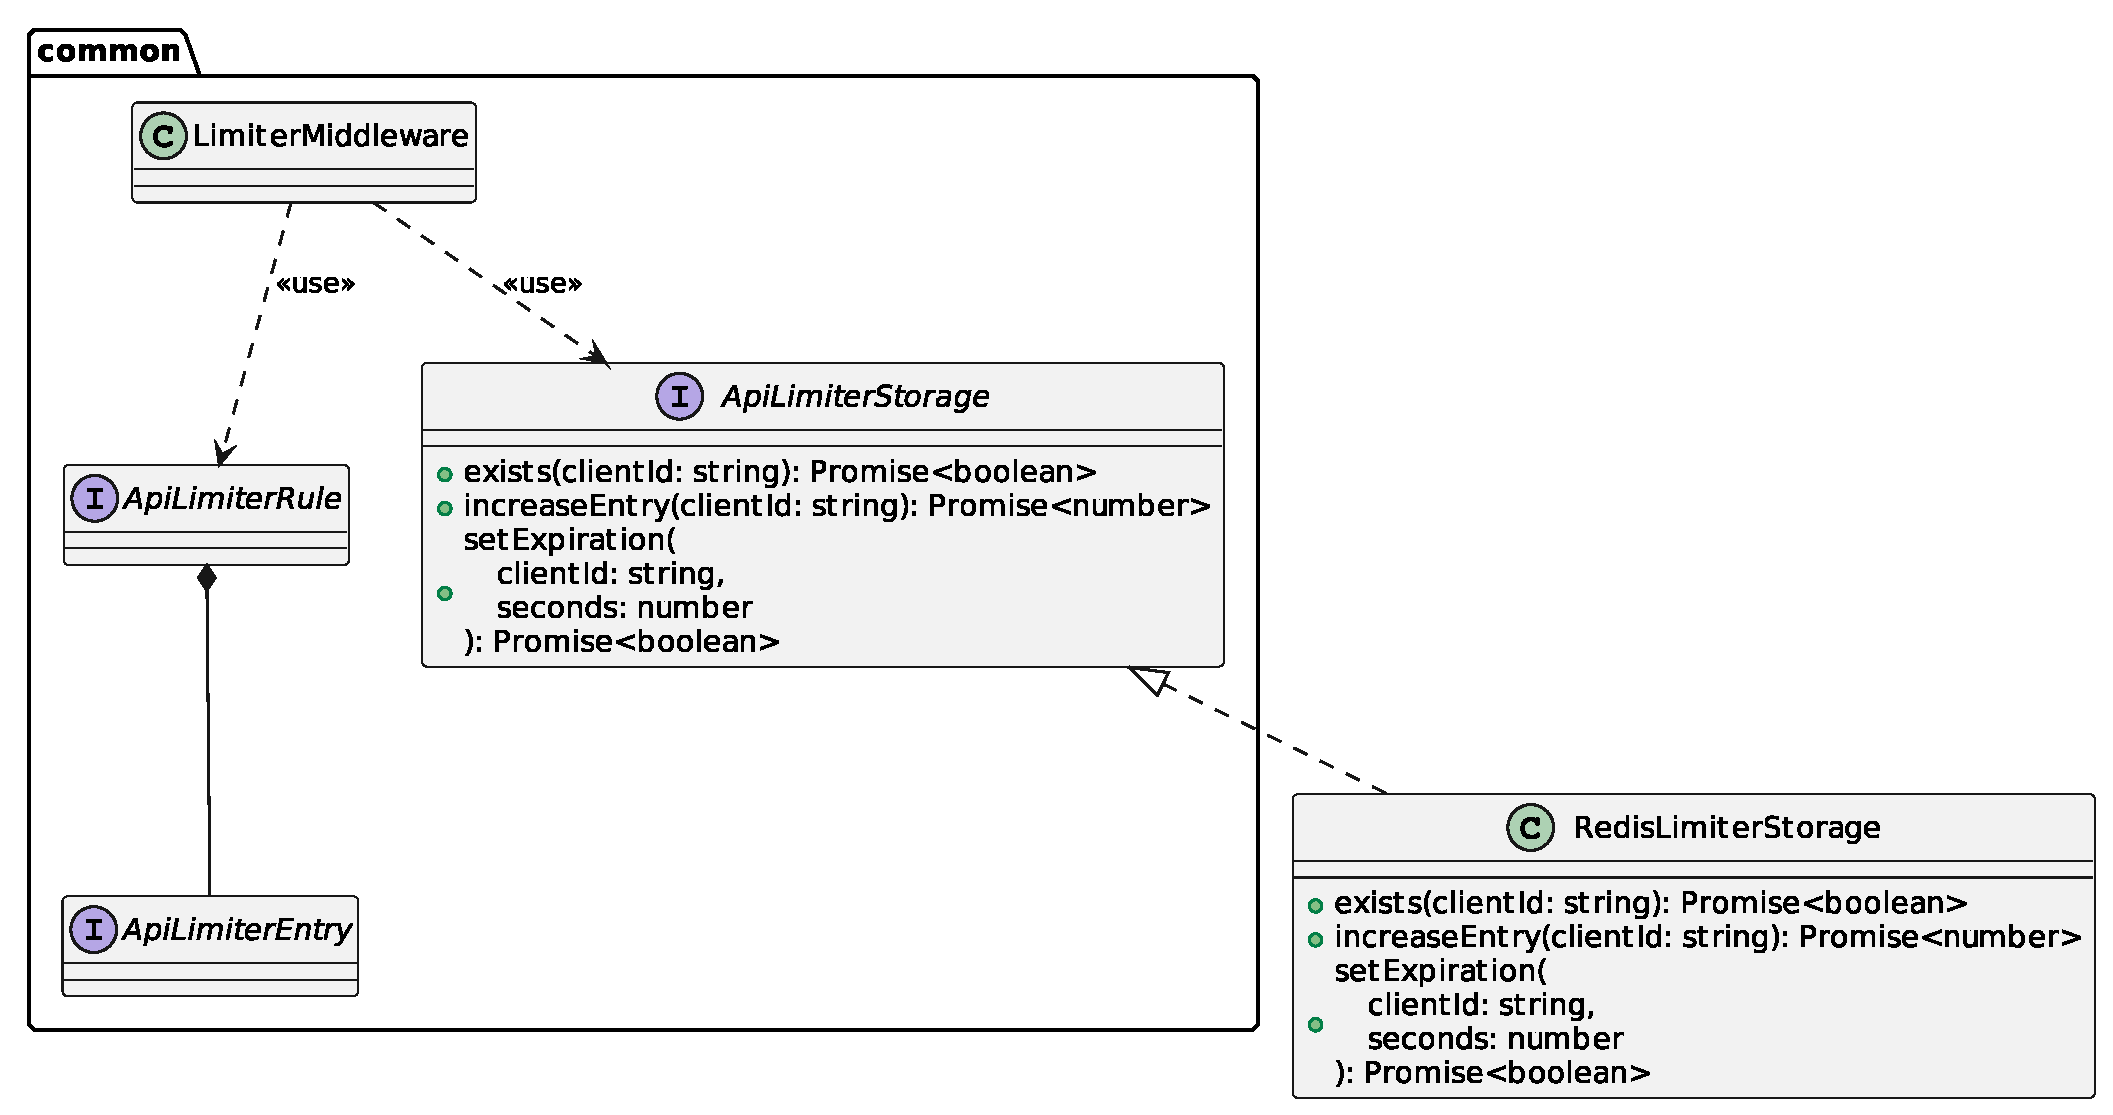
\includegraphics[width=\linewidth]{figures/api-limiter-api.eps}
    \label{fig:api-limiter-api} 
\end{figure}

\begin{info}[\textit{Documentation}]
    Here are listed the links where you can find the Open API documentation of both \texttt{:api-server} and \texttt{auth-server} modules:
    \begin{itemize}
        \item \href{https://tassiluca.github.io/ChainVote/swagger-ui-api/}{\texttt{:api-server} API}
        \item \href{https://tassiluca.github.io/ChainVote/swagger-ui-auth/}{\texttt{:auth-server} API}
    \end{itemize}
\end{info}

\fi
%% -------------------------------------- DS ----------------------------

\subsubsection{Authentication}
Authentication within the system is implemented by the use of \texttt{JWT tokens}. JWT \cite{jwt} is an open standard that allows the secure transmission of information between two parties as a JSON object. The information passed is digitally signed using the RS256 algorithm so it can be trusted and verified by an entity that requests it. Both the sign and verify functions for an access token are distributed to the \texttt{API} and \texttt{AUTH} server inside the \texttt{:common} package.

When a user tries to log in, the \texttt{AUTH} server will sign an access and a refresh token. The first one has a validity of 15 minutes while the latter one of 30, both will be securely signed by a private key and then sent back to the client. 

\jsimport[
    caption={The login method in the auth server},
    label={lst:login-auth-server}
]{listings/login.ts}

The client is responsible for securely storing the tokens and for sending them to the request that requires authentication. Before accessing the routes, \texttt{API} server verifies the validity of the access token and extract 
the information that it needs from it.
This operation is performed by a middleware that is executed before the request is processed by the route handler. It verifies the validity of the token and extracts the information that it needs from it. If the token is valid, the middleware registers the user information and sends it to the function that handles the request. If the token is not valid, the middleware sends back an error response.

\jsimport[
    caption={The middleware that handles the authentication},
    label={lst:auth-middleware}
]{listings/authentication.handler.ts}

\begin{figure}
    \centering
    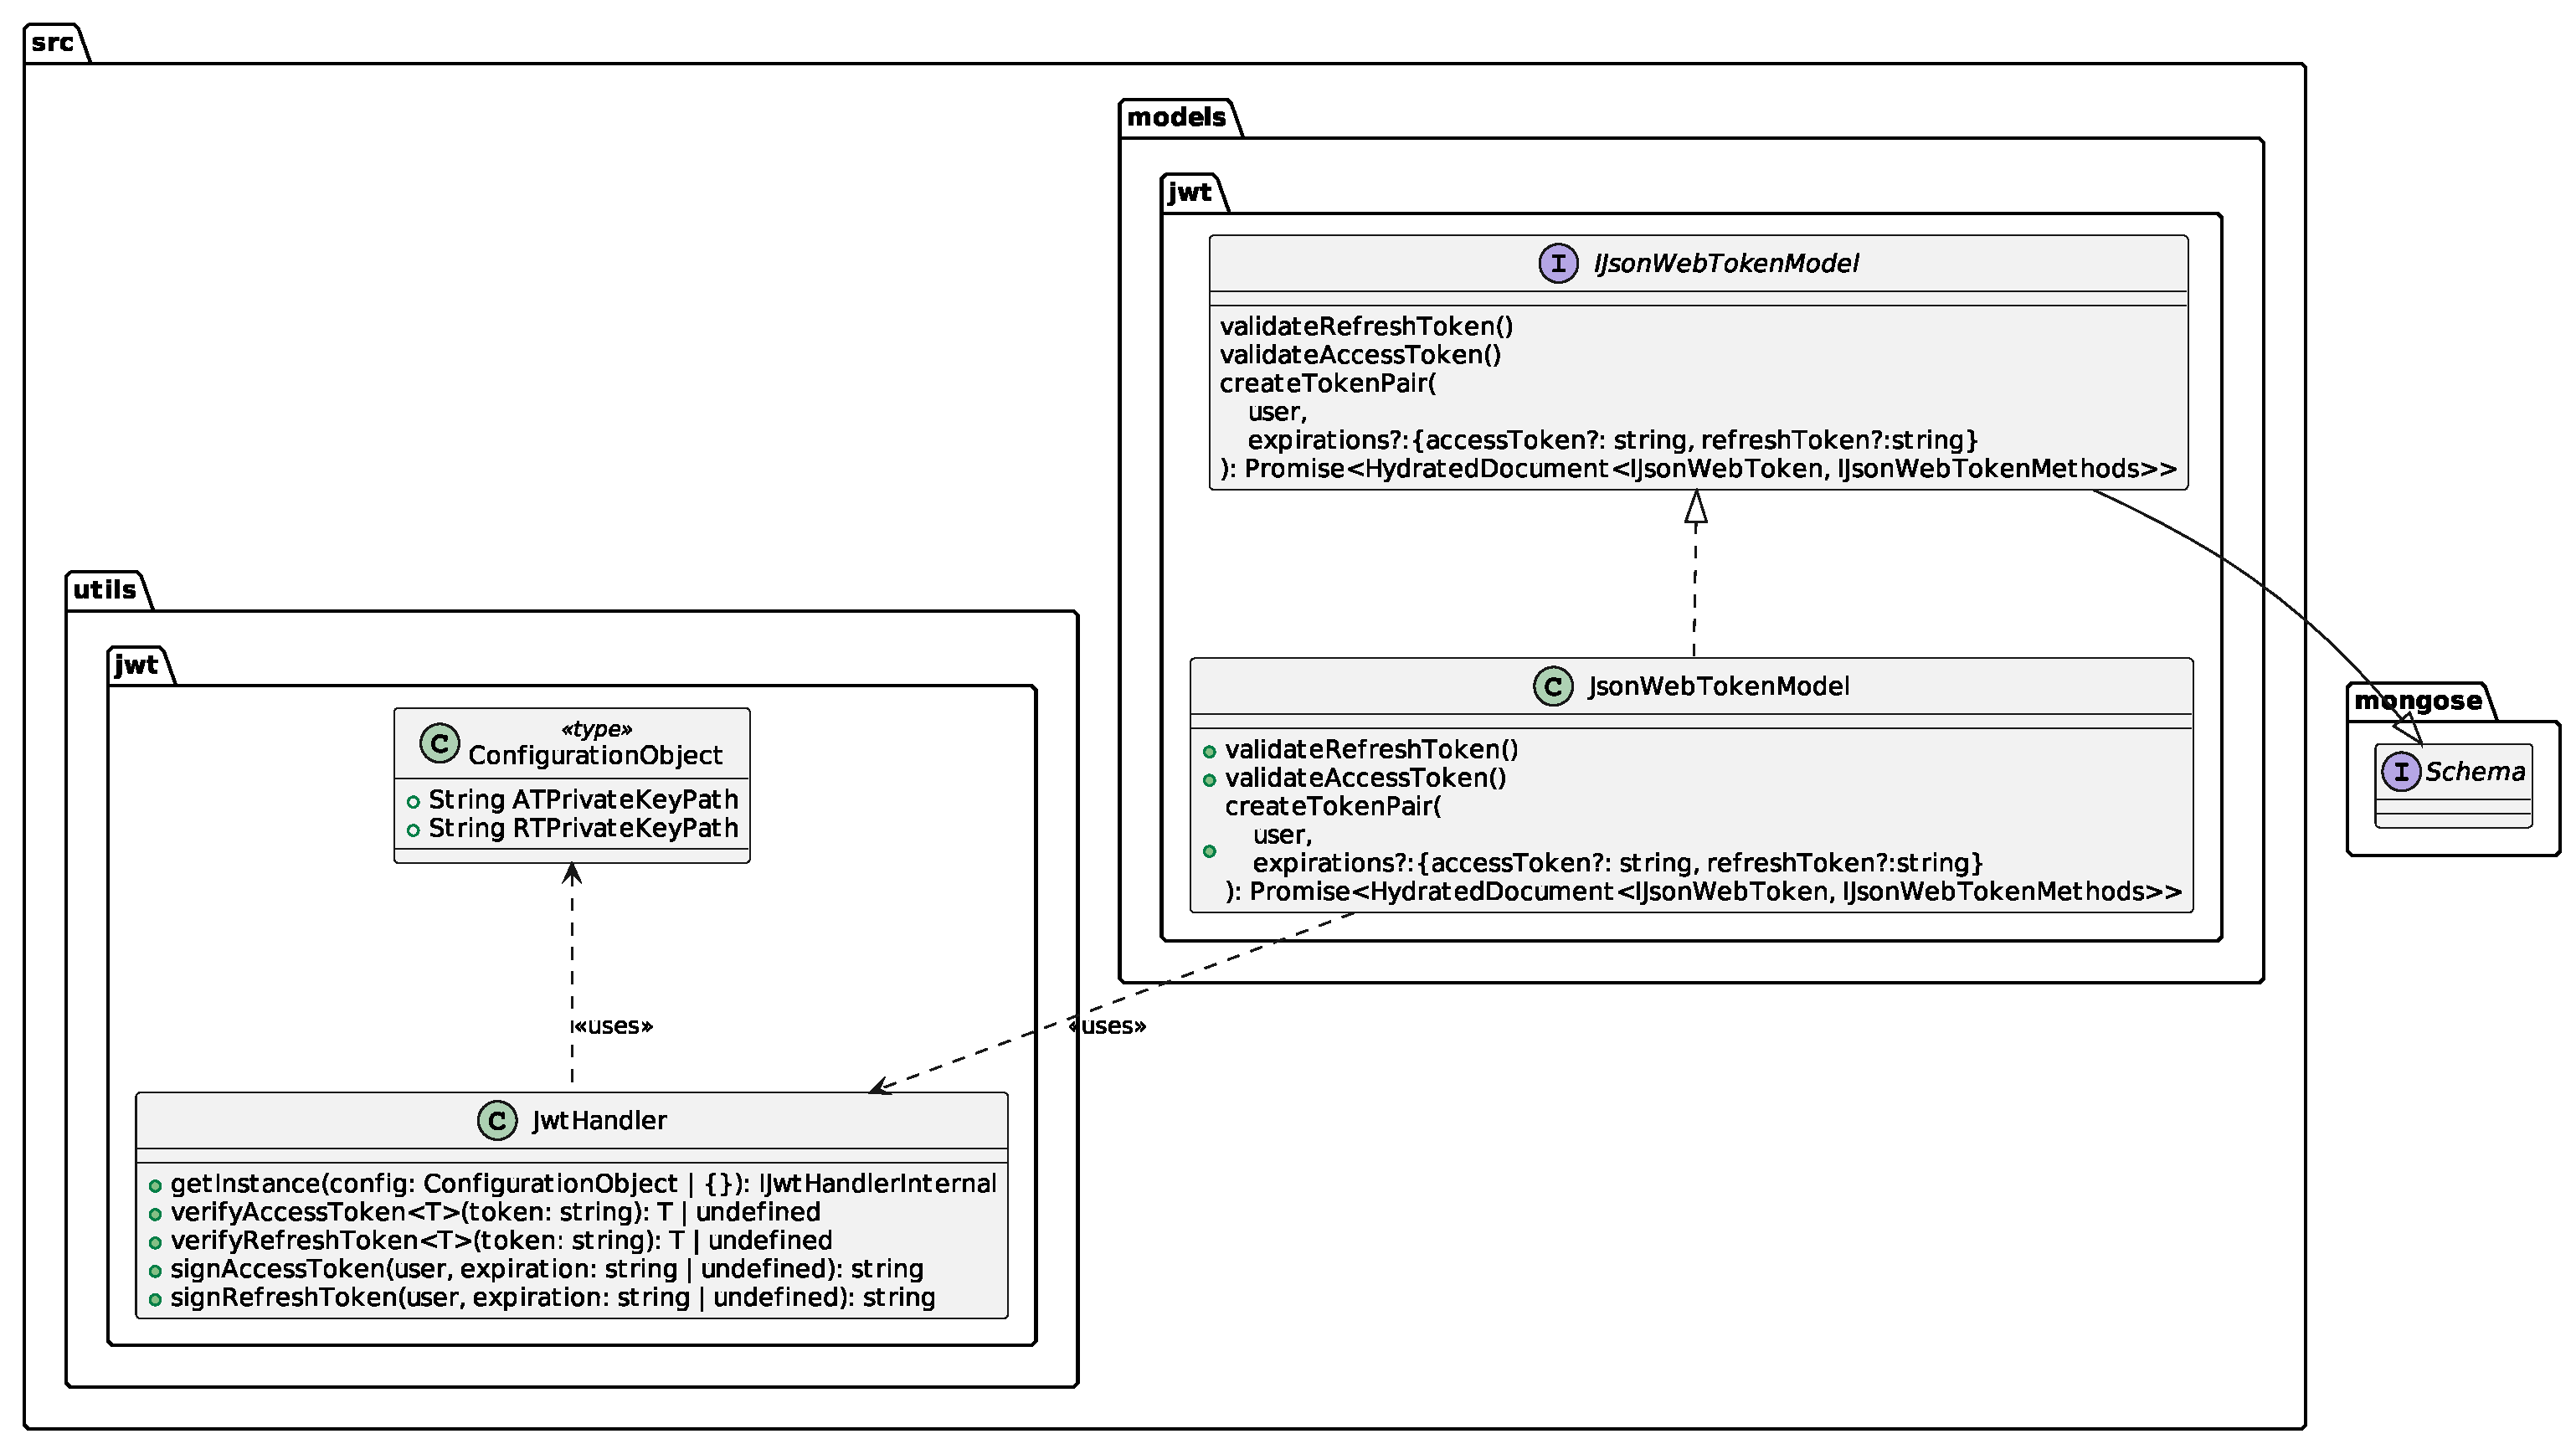
\includegraphics[width=\linewidth]{figures/jwt-api.eps}
    \label{fig:jwt-packages-api} 
    \caption{The overall API for the management of the JWT tokens}
\end{figure}

The \texttt{Jwt} model handles the verification and persistence of tokens inside the \texttt{MongoDB} database. It uses the namesake utility class, located within the \texttt{utils.jwt} package which is responsible for managing the construction of the various parts of the token.

\begin{warn}[\textit{Warning}]
    Once the network is deployed, the script copies a pair of public \& private keys in \texttt{api}, \texttt{auth} and \texttt{common} modules. While this operation simplifies the deployment process, and its testing, we're aware that in a real scenario, this would be a security issue and the private key should be stored and distributed relying on a more secure way.
\end{warn}

\subsubsection{Rate limiter}
We've implemented a custom rate-limiter module inside the API layer, which is responsible for limiting the number of requests that a client can send to a specific endpoint. This is done by using a \texttt{Redis} database that stores the number of requests that a client has sent to a specific endpoint. The rate limiter is implemented as a middleware that is executed before the request is processed by the route handler. It checks if the client has exceeded the maximum number of requests allowed, if so it sends back an error response to the client, otherwise, it increments the number of requests and sends the request to the route handler.

The way it works is as follows: each controller specifies a set of rules for each endpoint that can vary from the type of request.

\jsimport[
    caption={The definitions of the rules for the rate-limiter},
    label={lst:rate-limiter-rules}
]{listings/api.rule.ts}

In \Cref{lst:rate-limiter-rules} we listed the rules for three endpoints, each of them specify for the \texttt{verb} type two parameters:
\begin{itemize}
    \item \texttt{time}: The time window in which the requests are counted.
    \item \texttt{limit}: The maximum number of requests that can be sent in the specified time window.
\end{itemize}

So, for example, \texttt{endpoint\_name\_1} can receive a maximum of 50 requests in 18 seconds if the request type is \texttt{POST} and 60 requests in 14 seconds if the request type is \texttt{GET}.
The set of rules is then passed to the RateLimiter middleware which retrieves the IP address of the client and the endpoint that is being requested. 
Route checking is done on data saved on a \texttt{Redis} database. To make this solution more modular and extensible a Storage (\texttt{ApiLimiterStorage}) interface was devised that defines the operations to be performed on the data. 

\jsimport[
    caption={The limiter middleware},
    label={lst:rate-limiter-middleware}
]{listings/api.limiter.ts}

\begin{figure}
    \centering
    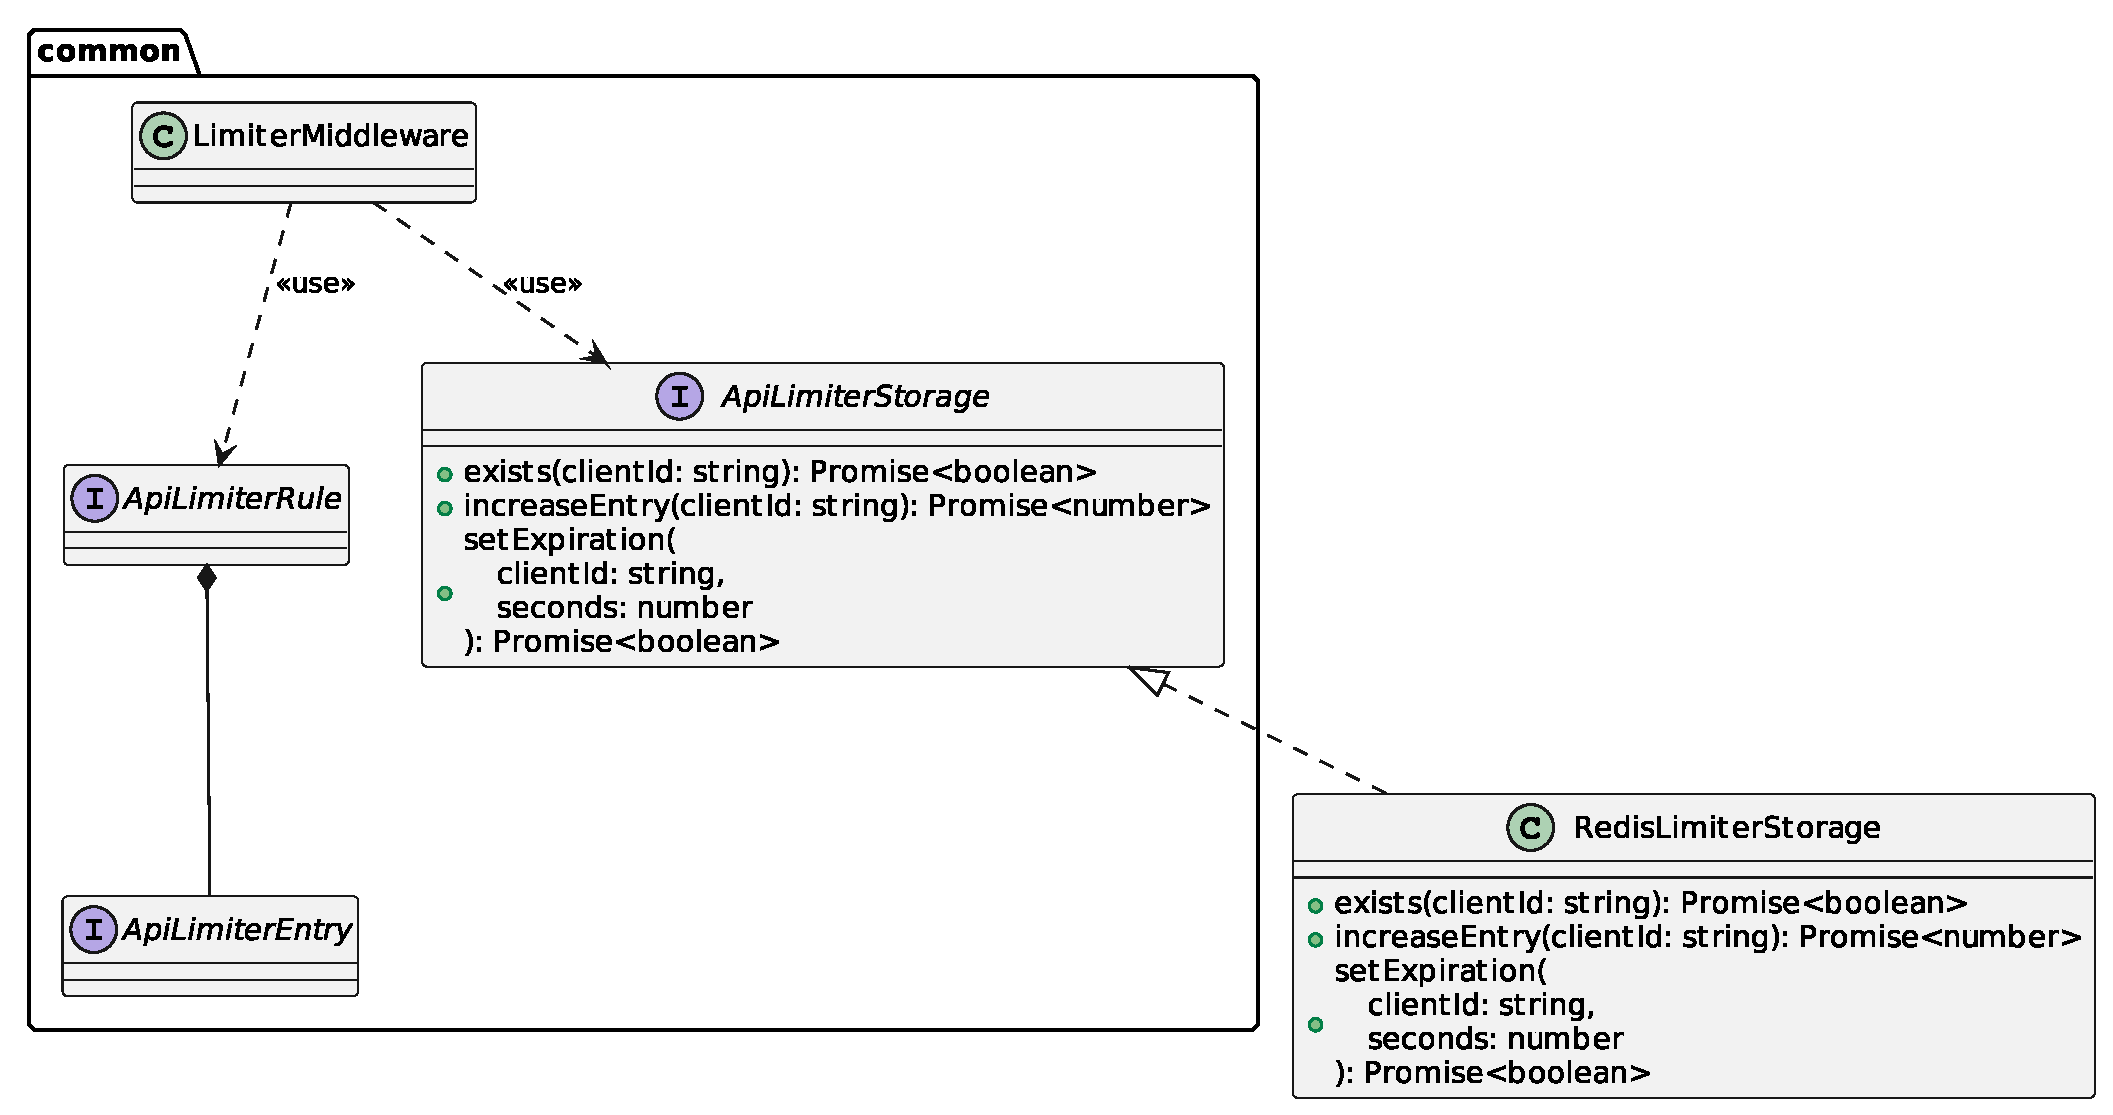
\includegraphics[width=\linewidth]{figures/api-limiter-api.eps}
    \label{fig:api-limiter-api} 
\end{figure}

\subsubsection{Mailer}

\subsubsection{Routes}

Following REST principles, we defined routes according to the main entities.
Using Open API, we provide documentation of both \texttt{:api-server} and \texttt{auth-server} modules:
\begin{itemize}
    \item \href{https://tassiluca.github.io/ChainVote/swagger-ui-api/}{\texttt{:api-server} API}
    \item \href{https://tassiluca.github.io/ChainVote/swagger-ui-auth/}{\texttt{:auth-server} API}
\end{itemize}

A brief example is provided in \Cref{fig:backend-routes}.

\todo{Check if it's okay}

\begin{figure}
    \centering
    \begin{subfigure}[b]{0.3\textwidth}
        \centering
        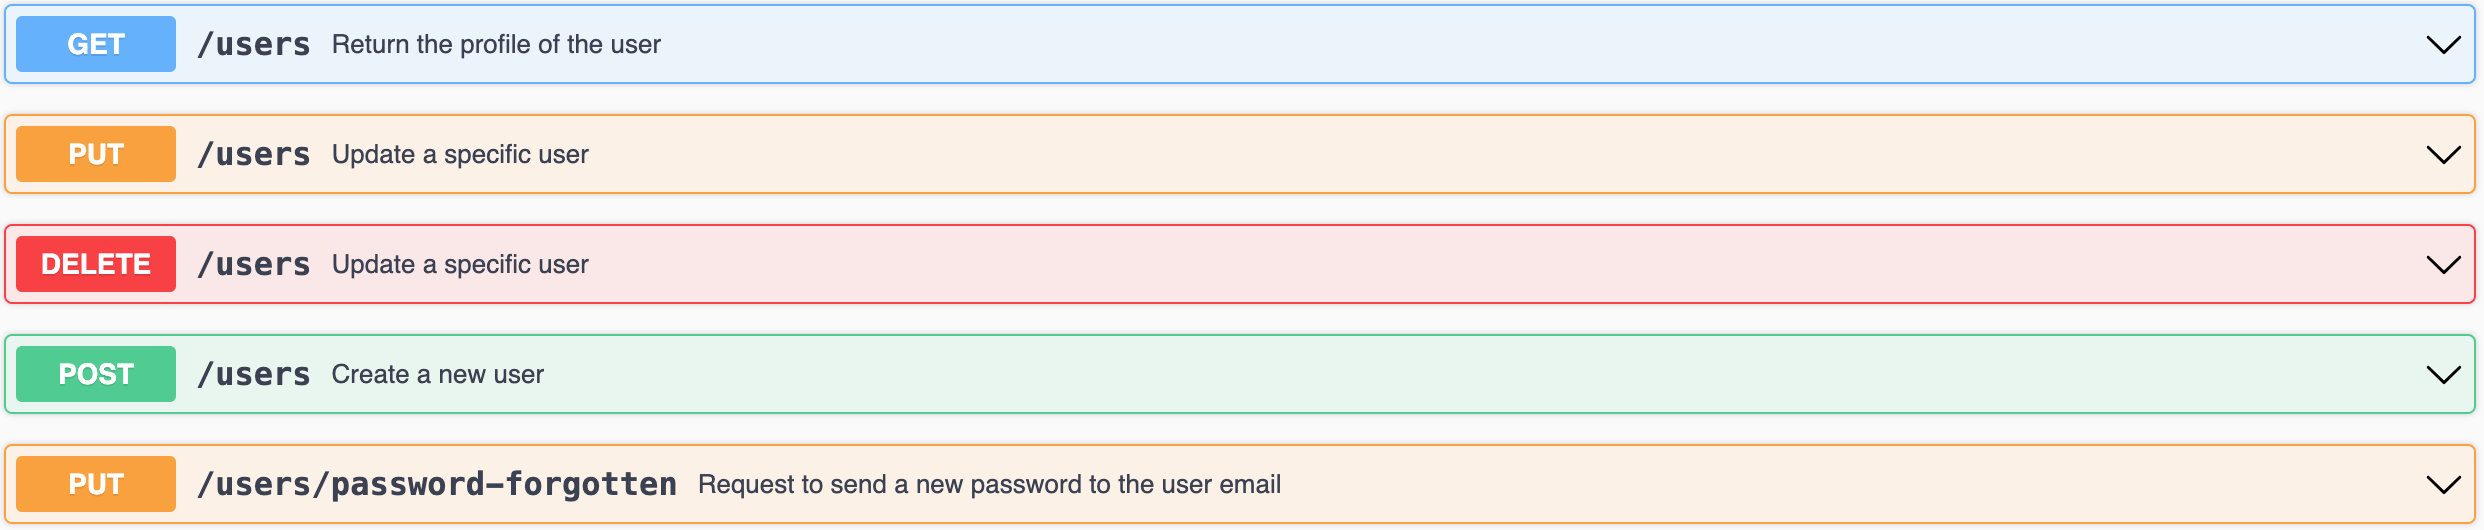
\includegraphics[width=\textwidth]{./figures/backend-routes/users.png}
        % \caption{}
    \end{subfigure}
    \hfill
    \begin{subfigure}[b]{0.3\textwidth}
        \centering
        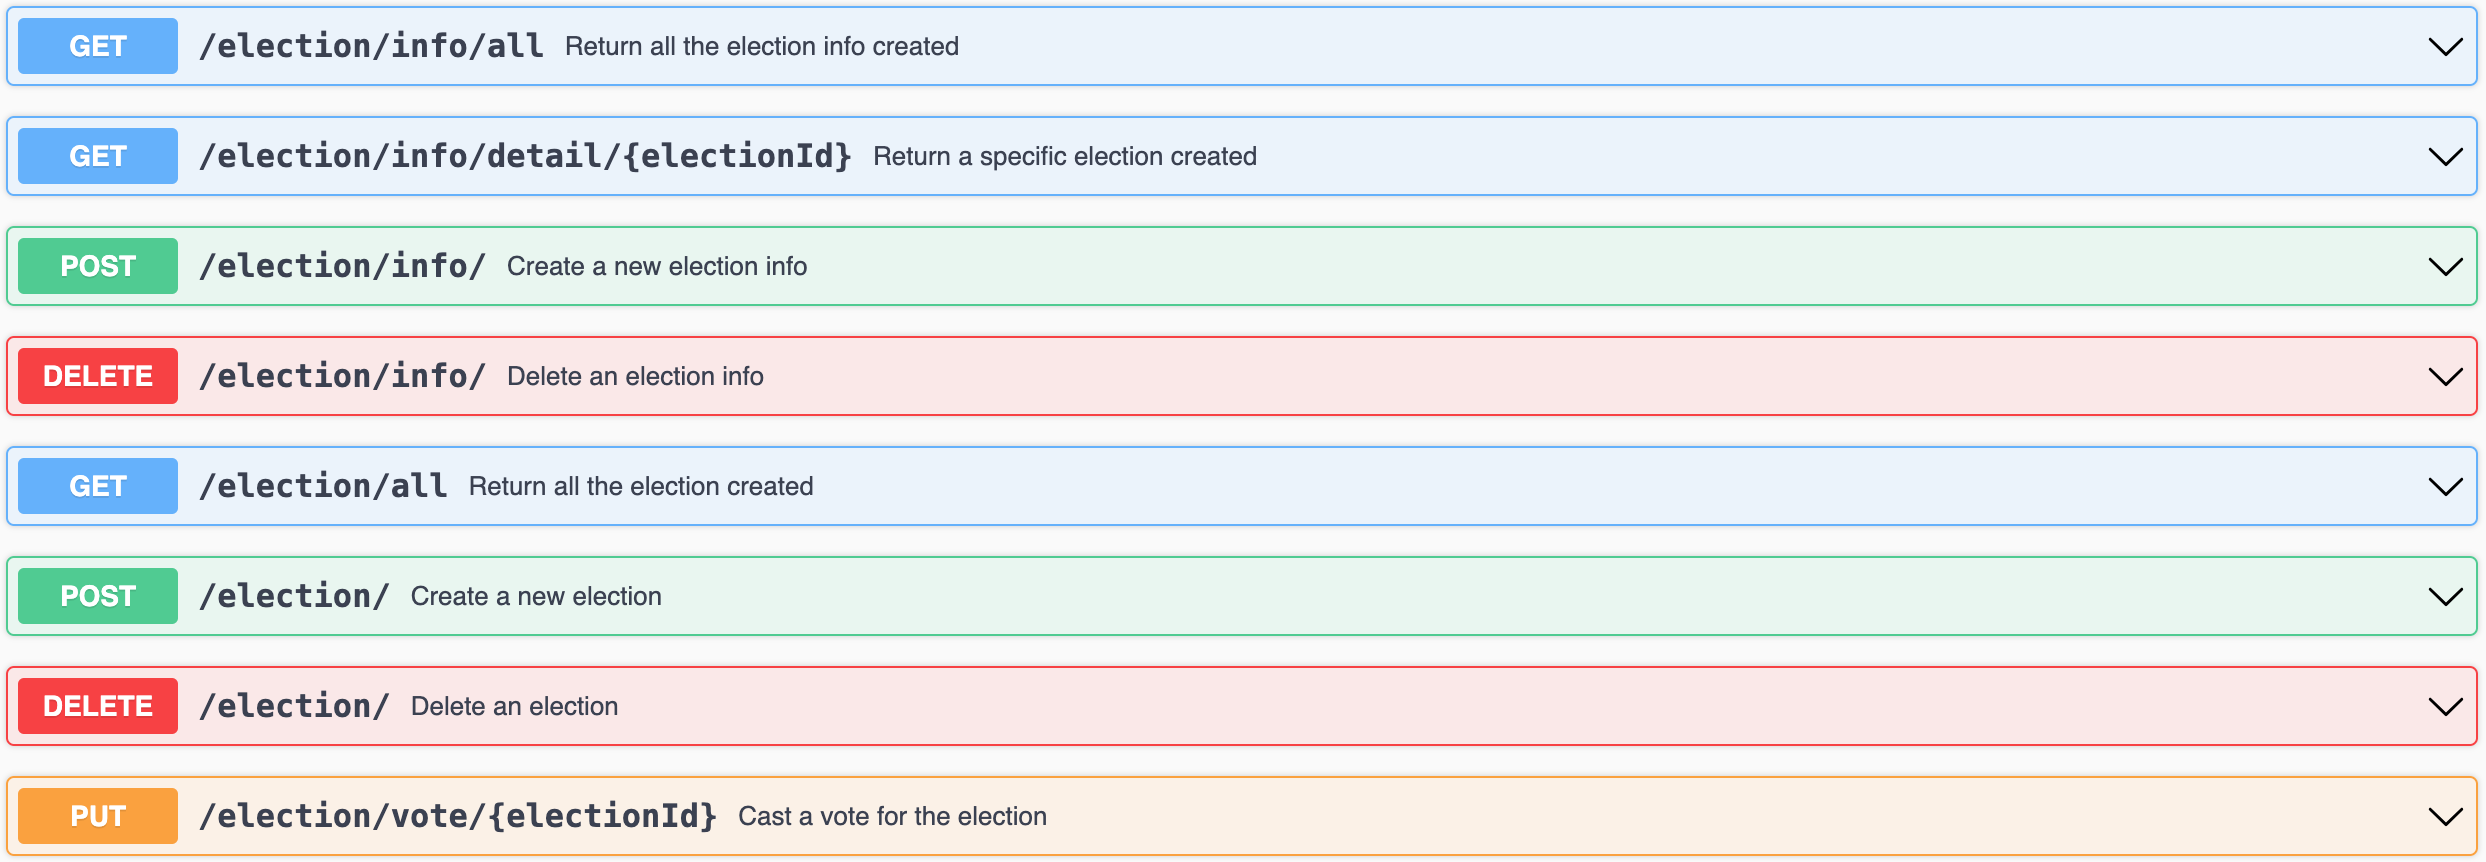
\includegraphics[width=\textwidth]{./figures/backend-routes/election.png}
        %\caption{}
    \end{subfigure}
    \hfill
    \begin{subfigure}[b]{0.3\textwidth}
        \centering
        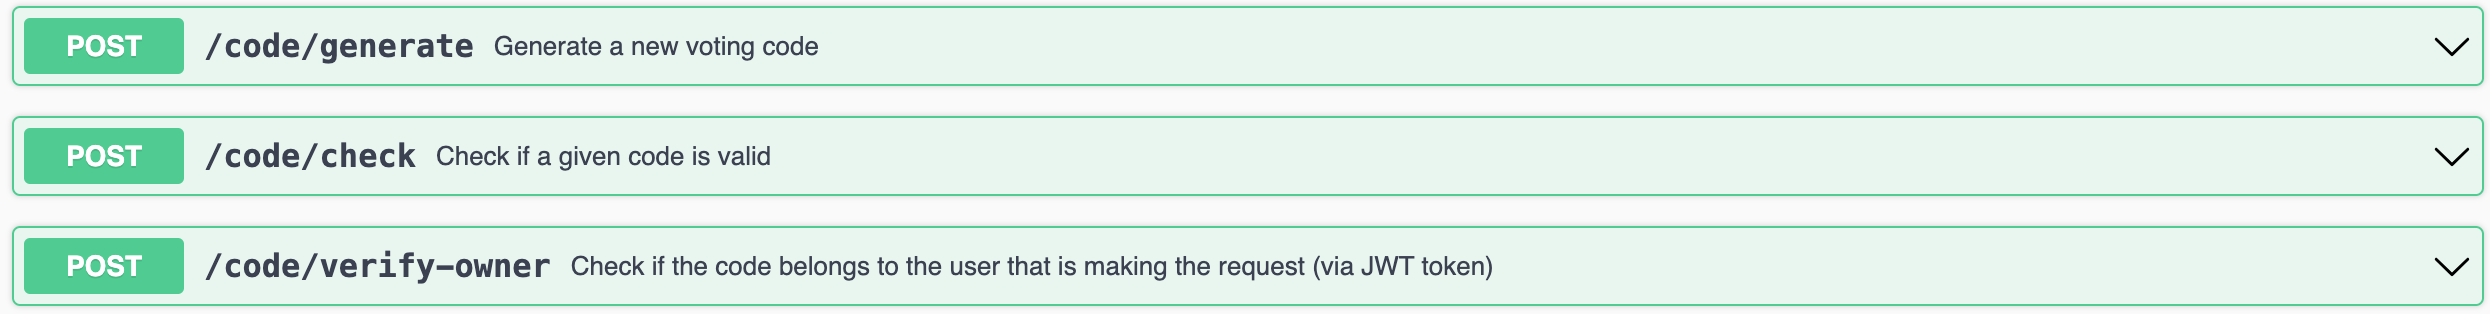
\includegraphics[width=\textwidth]{./figures/backend-routes/code.png}
        %\caption{}
    \end{subfigure}
    \hfill
    \begin{subfigure}[b]{0.3\textwidth}
        \centering
        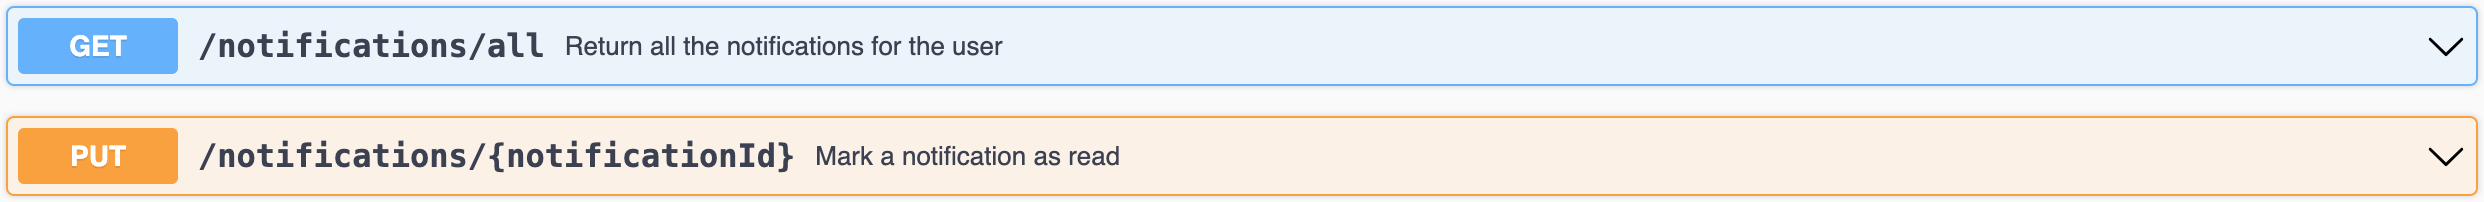
\includegraphics[width=\textwidth]{./figures/backend-routes/notifications.png}
        %\caption{}
    \end{subfigure}
    \hfill
    \caption{Backend routes api.}
    \label{fig:backend-routes}
\end{figure}

\subsubsection{Real time updates and notifications with \texttt{Socket.io}}

\texttt{Socket.io}, as already stated in \Cref{sec:technologies}

\subsection{Frontend}

\subsubsection{Stores}

We've collected all backend APIs in stores, one for each main entity of the system, which also hold information required in communications.

\subsubsection{Vue Components}

Given the reusable and modular nature offered by Vue's component, we've implemented several components to manage custom content and logic.
By means of custom emit events and props, the nested structure offered by components can be crossed from parent to child components bidirectionally, triggering events in child components that propagate up to the parents.

\section{Story board}


\section{Validation}

%% -------------------------------------- DS ----------------------------
\iffalse

Tests have been conducted on different levels: domain model, smart contracts and API interactions.

Concerning the domain model of the smart contract unit test has been used (using JUnit framework \cite{junit}).
%
They can be found in \texttt{:core} module.

To test smart contracts, since their functioning requires the network to be up and running, and to effectively bring up the network requires a non-negligible time which would have made the testing environment viscous, Mockito framework \cite{mockito} has been adopted to mock the network-dependent parts.
%
Indeed, Mockito allows the creation of mock objects, which essentially are placeholders for real objects that simulate their behavior by defining the expected outcome provided by specified methods, and spy objects which allow a partial mock of some method of an existing object, retaining its original behavior while customizing certain aspects.
%
An example of usage for the 

\javaimport[
    caption={An example of Mockito behavior definition},
    label={lst:mockito-example}
]{listings/MockitoExample.java}

\javaimport[
    caption={An example of Mockito Spy behavior definition},
    label={lst:mockito-spy-examlpe}
]{listings/MockitoSpyExample.java}

Some testing metrics regarding \texttt{smart-contracts module}: a total of 86 tests were developed, including \texttt{core}, \texttt{presentation} and \texttt{chaincode*} submodules, and the test coverage is overall higher than 80\% (the detail is shown in \Cref{fig:smart-contracts-coverage}).

\begin{info}[\textit{Tests}]
    To run the smart contracts tests, simply: \texttt{./gradlew test} inside the \\ \texttt{smart-contracts} folder of the project.
    \\
    Reports are available in each \texttt{build/reports/tests} submodule directory.
\end{info}

\begin{figure}
    \centering
    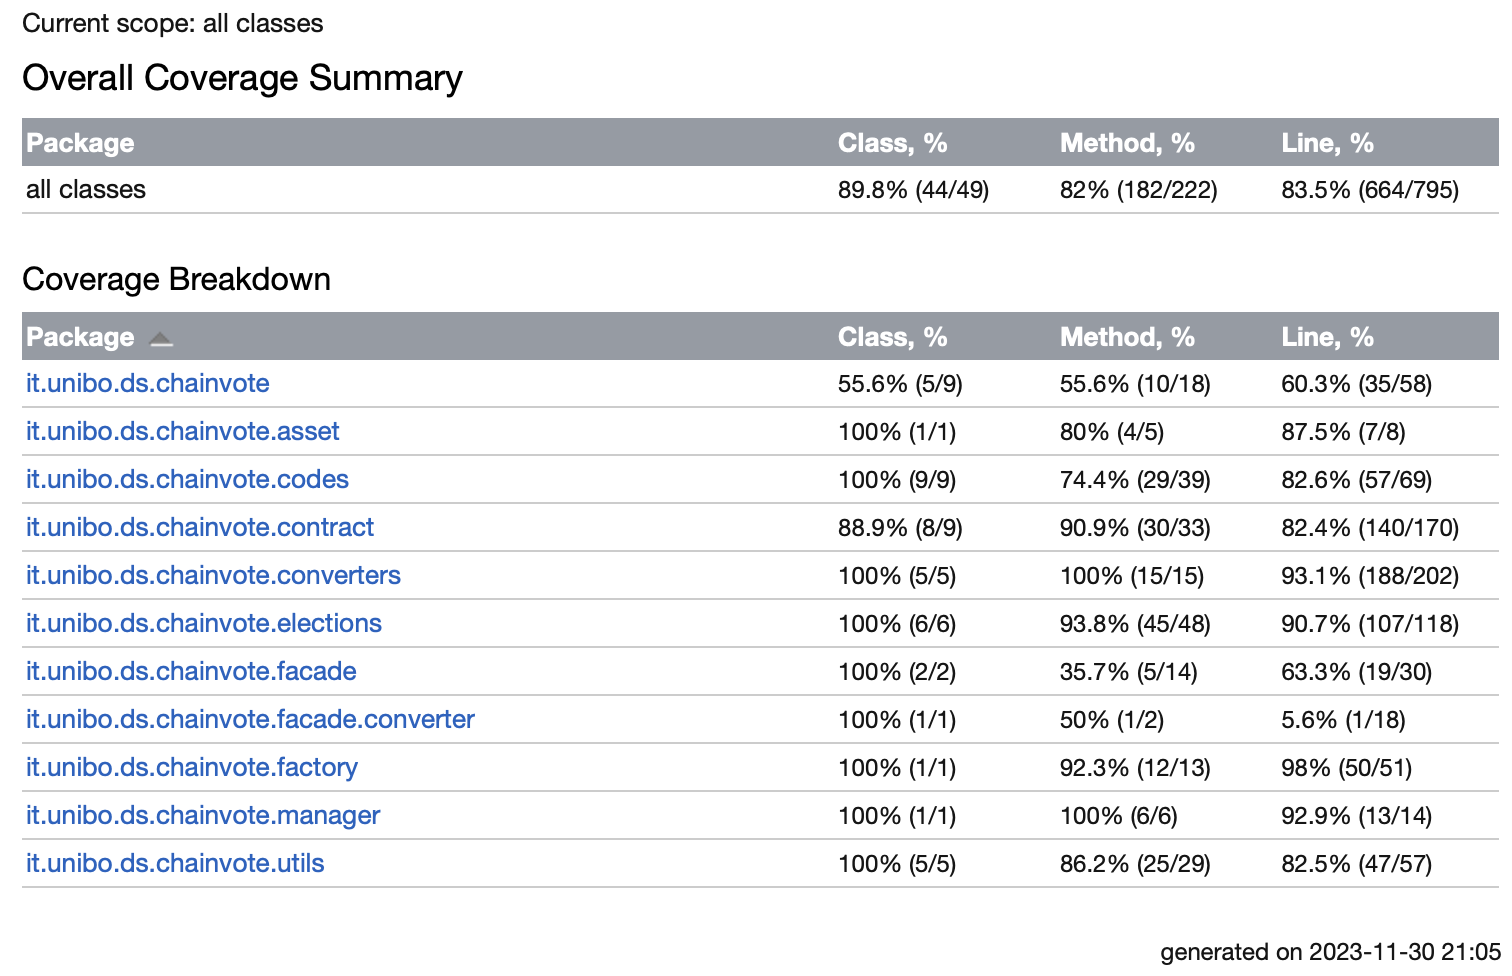
\includegraphics[width=\linewidth]{figures/smart-contracts-coverage.png}
    \caption{Coverage of the \texttt{:smart-contracts} module.}
    \label{fig:smart-contracts-coverage} 
\end{figure}

Concerning distributed quality attributes of the blockchain component, such as fault tolerance, we leverage the Hyperledger Fabric framework which ensures that, for example, if a peer is down, the transactions are redirected to the other peers of the organization.
%
Manual tests have been conducted to stress the network in corner cases (like the one cited above) operating on the peers' containers.

\subsection{API Testing}
The principal goal of the API testing is to verify that the server correctly handles the requests that it receives from the client. To achieve this we used in combination the \texttt{jest} testing library along with \texttt{supertest}. The first one is a JavaScript testing framework that allows the creation of unit tests for JavaScript code, while the latter is a library that allows the creation of HTTP requests to a server

\jsimport[
    caption={An example of an API test},
    label={lst:jest-test}
]{listings/jest.example.ts}

In \Cref{lst:jest-test} we show an example of testing on POST requests to the /code endpoint of the API server. \texttt {jest} allows control division \& execution of the tests introducing initialization and cleanup functions that will be executed before and after the execution of the tests. 
We can group up tests with \texttt{describe} functions, so we can better organize them among the various scenarios of the specific endpoints.
\texttt{request} is a function provided by the \texttt{supertest} library that allows the creation of HTTP requests to a server. It takes as input an instance of the express application, then we can configure it specifying the type of the request and the various parameters.

We check the validity of the response by evaluating the status code and the body of the response. 

\fi
%% -------------------------------------- DS ----------------------------

\section{Deployment}

\subsection{Prerequisites}

\begin{itemize}
    \item Unix-like operating system (either macOS or Linux);
    \item Docker and Docker Compose (on Mac OS make sure the file sharing implementation for the container is set to \texttt{osfx (Legacy)} (\texttt{Settings -> General});
    \item Java 11 or higher;
    \item Node.js 18 or higher;
    \item npm.
\end{itemize}

\subsection{Startup}

To bring up the blockchain network, deploy the smart contracts on top of the peers, start the API services and the frontend web app you can use the \texttt{services.sh} script on the root of the project.

To bring up all the system's services:

\begin{verbatim}
    ./services up
\end{verbatim}

Since the first time it will pull Hyperledger Fabric binaries and docker images to create blockchain artifacts and start API services, it will take a while to bring up the entire system.

While it reaches the API server creation phase, the script will execute the \texttt{npm login} command; we've preconfigured some default credentials for this purpose, these should be used when the login request is prompted:
\begin{itemize}
    \item username: \texttt{user}
    \item password: \texttt{password}
\end{itemize} 

\begin{warn}
    During the startup phase of the API layer, the script will require the sudo privileges in order to ensure that the \texttt{verdaccio}, \texttt{cache} and \texttt{dbdata} folders have write and read permissions, which are needed on Linux environment.
\end{warn}

The full working system consists of 33 containers (\Cref{fig:containers}): one for each peer and chaincode deployed on it, five containers for the API services and one for the frontend web app.

\begin{figure}[h!]
    \centering
    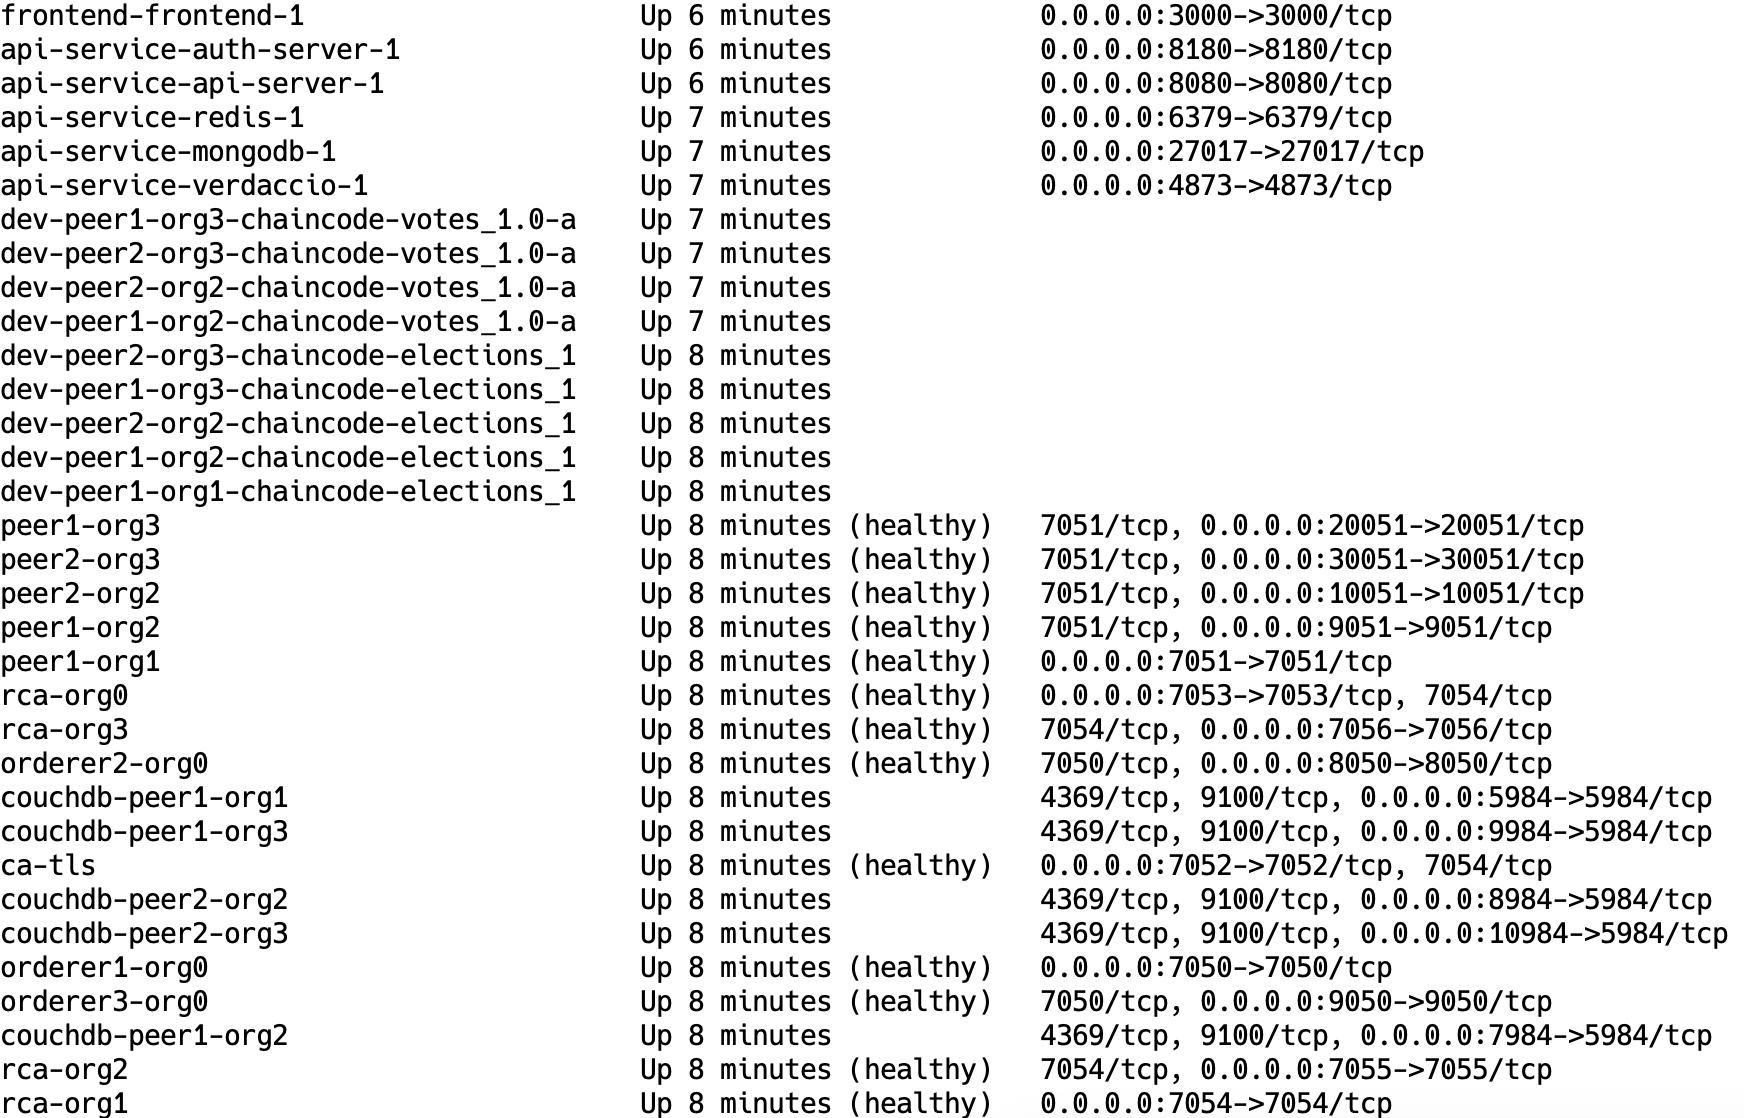
\includegraphics[width=\linewidth]{figures/containers.png}
    \caption{The set of containers that should be up and running at the end of the deployment.}
    \label{fig:containers} 
\end{figure}

To bring them down without cleaning the blockchain artifacts (it will speed up the creation of the network next times):

\begin{verbatim}
    ./services down
\end{verbatim}

To clean network artifacts:

\begin{verbatim}
    ./services clean
\end{verbatim}

%% -------------------------------------- DS ----------------------------
\iffalse

\subsection{Details}
\label{deployment-details}

Each project's module is shipped with a script that automatizes its subpart of the system.
%
\texttt{services.sh} script, under the hood, sequentially executes each module's deployment script in order to make the deployment of the entire system simpler.

\subsubsection*{\texttt{:blockchain} module}

For this module a \texttt{network.sh} bash script automatize the deployment of the blockchain network and all its component.
%
It has been built following the Fabric CA Operations Guide \cite{hyperledger-fabric-ca-docs} \cite{fabric-ca-rework}, simulating its deployment using Docker.

The overall process is non-trivial and it is summarized in \Cref{fig:blockchain-up-sequence}.

\begin{figure}
    \centering
    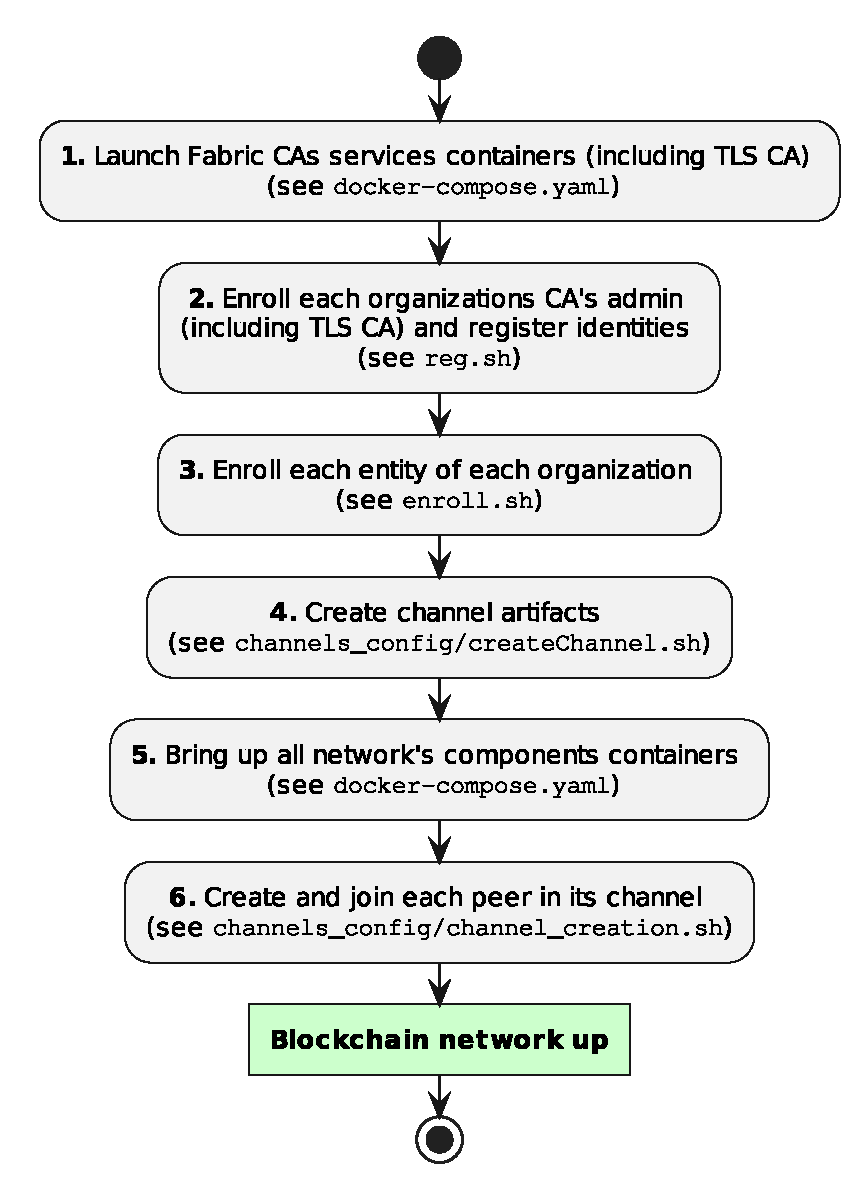
\includegraphics[width=0.6\linewidth]{figures/blockchain-up-sequence.eps}
    \caption{A sequence diagram representing the steps required to create the blockchain network.}
    \label{fig:blockchain-up-sequence}
\end{figure}

After bringing up all the CA's service containers, including the TLS-CA one, (step 1) for each of them an admin is enrolled using the \texttt{fabric-ca-client} script of Hyperledger Fabric.
%
This admin is used to register each entity into the CA database, which will be used in subsequent steps during the enrollment of these entities.
%
These procedures are executed within the \texttt{reg.sh} script (step 2).
%
The enrollment of each entity (both network components and users) from the Certificate Authorities (CAs) is now undertaken for each organization in \texttt{enroll.sh} (step 3).
%
Then, the channel artifacts are generated (step 4) using the \texttt{configtxgen} script provided by Hyperledger Fabric from the configuration files described in \Cref{sec:blockchain-network-impl}.
%
Once the channel artifacts have been created all the network components containers are brought up, the channel is created and peers join them (steps 5 and 6).

All the network components containers are deployed through Docker Compose (using the \texttt{docker-compose.yaml} file in the \texttt{:blockchain} module folder).

\subsubsection*{\texttt{:smart-contracts} module}

The \texttt{:smart-contract} module provides a set of Gradle tasks created to bring up the network, package the chaincodes and install them on the peers.
%
These are shown below (to list them: \texttt{./gradlew tasks}):

\begin{verbatim}
    Blockchain tasks
    ----------------
    cleanAllPackages - Remove all generated packages
    downNetwork - Bring down the blockchain network without cleaning
                  artifacts
    downNetworkAndClean - Bring down the blockchain network and clean
                          the artifacts
    packageChaincodes - Build and generate chaincodes packages
    upAndDeploy - Up the network and deploy chaincodes in one shot
    upNetwork - Bring up the blockchain network
\end{verbatim}

Among others, \texttt{upAndDeploy} is the Gradle task which automatizes the upping of the network and the installation of both chaincodes in one single shot.

Technically, the installation of a chaincode on peers involves, after creating the network, the following steps (\Cref{fig:sc-installation-sequence.eps}):

\begin{enumerate}
    \item Build and generate chaincodes jars;
    \item Package the jars into a \texttt{.tar.gz} files with the \texttt{peer lifecycle chaincode package} command;
    \item Install the chaincodes on every peer that will endorse a transaction with the \texttt{peer lifecycle chaincode install} command;
    \item After the installation, the organization's approval is needed. The set of channel members who need to approve a chaincode before it can be deployed is governed by the \texttt{Application/Channel/LifecycleEndorsement} policy described in \Cref{sec:blockchain-network-impl};
    \item After a sufficient number of organizations have approved a chaincode definition, one organization can commit the chaincode definition to the channel using the \texttt{peer lifecycle chaincode commit} command.
\end{enumerate}

\begin{figure}
    \centering
    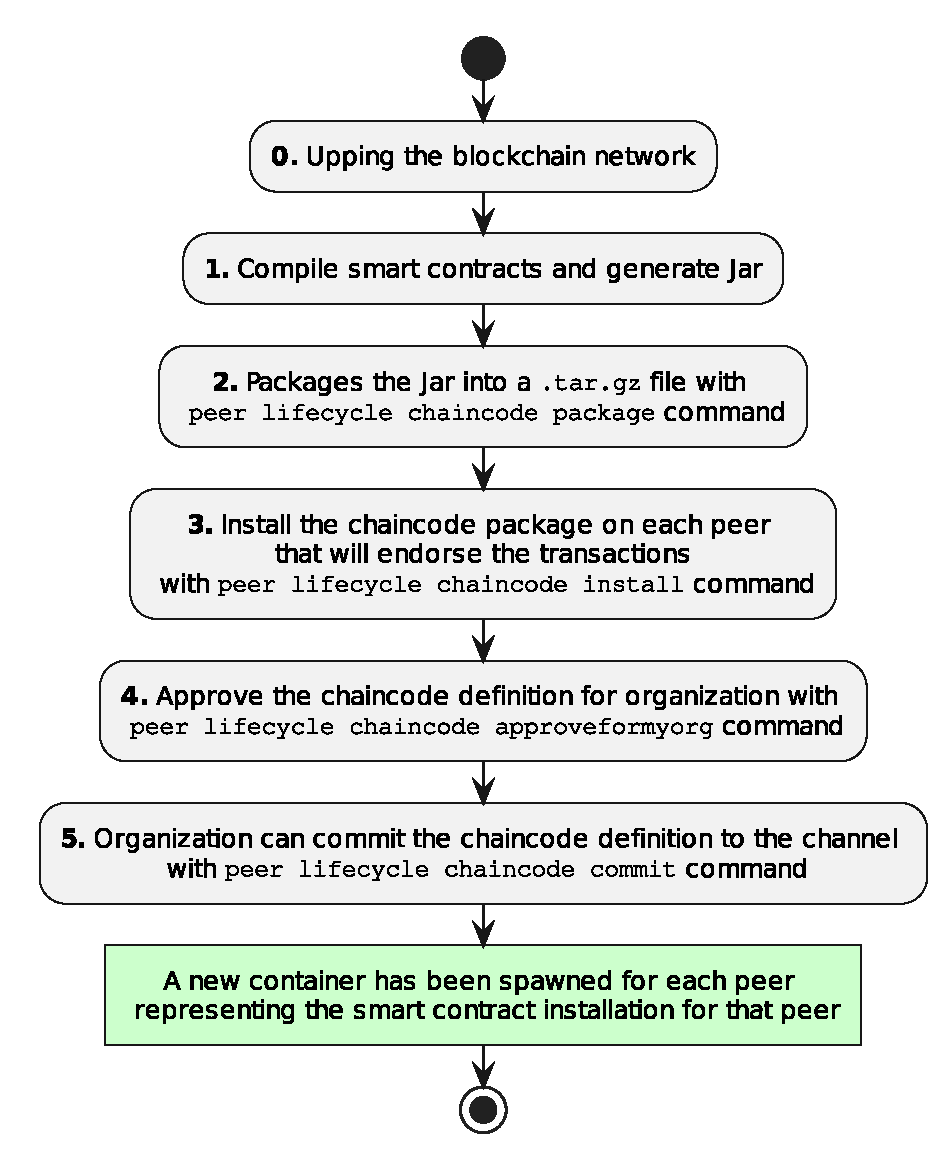
\includegraphics[width=0.7\linewidth]{figures/sc-installation-sequence.eps}
    \caption{A sequence diagram representing the steps required to install the chaincodes on top of the peers.}
    \label{fig:sc-installation-sequence.eps}
\end{figure}

All of these steps have been programmed in Kotlin within Gradle tasks into the \texttt{build.gradle.kts} project's build file.

Moreover, since the startup of the network and the chaincodes installation is a very critical asset for the project a CI Pipeline has been set up to test its functioning at every pushed commit on a \href{https://github.com/tassiLuca/ChainVote}{mirrored repository} hosted on GitHub.

\subsubsection*{\texttt{:api-service} module}

We deploy all the services inside the \texttt{:api-service} module using a simple script called \texttt{startup.sh}. This contains two functions: 
\begin{itemize}
    \item \texttt{up} which will prepare the environment and start the API servers;
    \item \texttt{down} which will stop the API layer.
\end{itemize} 

When the \texttt{up} is executed it will first copy a pair of test keys inside the \texttt{common},\texttt{auth},\texttt{api} folders, these are used for testing the jwt functions. 
After that it creates the data folders that should be used as mounting points for verdaccio and redis: \texttt{dbdata} and \texttt{cache}. 
After that, using the docker-compose yaml file, the \texttt{Verdaccio} server will be started and the common dependencies, inside the \texttt{:common} package will be built and published on the local registry.
Once the dependencies are published the rest of the services are built and started. The \texttt{down} function will simply stop the API layer using the \texttt{docker-compose down} function.

\subsubsection*{\texttt{:frontend} module}

The \texttt{:frontend} module contains just a \texttt{docker-compose.yaml} file thanks to which, simply with \texttt{docker compose up}, the frontend container can be started, listening on port \texttt{3000}.

\fi
%% -------------------------------------- DS ----------------------------

\subsection{Troubleshooting}
If you are encountering issues or observing unexpected behavior during the deployment, this troubleshooting guide is designed to assist you in identifying and resolving common problems.

\subsubsection*{Linux/MacOS: \texttt{[common.tools.configtxgen] main -> Error on outputBlock: could not create bootstrapper: could not create channel group ...: open /Projects/distributed-systems/ds-project/chain-vote/blockchain/ \\../.chainvote/blockchain/org0/orderer1/tls-msp/signcerts/cert.pem: no such file or directory}}

A similar error occurs the next time a problem arises during the creation of channel artifacts because it tries to get some files inside the artifacts folder but, since the previous deployment failed, those files don't exist.
%
Cleaning the artifacts with \texttt{./services clean} should solve the problem.

\subsubsection*{MacOS: resource management}
On MacOS systems make sure to increase allocated resources in Docker Desktop, particularly for CPU and memory limit (8GBs are enough).

\subsubsection*{MacOS: \texttt{Error response from daemon: cannot stop container: <container-id>: tried to kill container, but did not receive an exit event}}

Sometimes happens that, when the services are torn down (with \texttt{./services down} or \texttt{services clean}), one Hyperledger CA container remains hanging.
Restarting Docker Desktop solves this issue.

\subsubsection*{MacOS: \texttt{container peer1-org2 is unhealthy}}
If, during the deployment of the network, the shown message (or a similar one) appears on a MacOS host, make sure the file-sharing implementation for the containers in \texttt{Settings -> General} is set to \texttt{osxfs (Legacy)}.

\subsubsection*{MacOS/Linux: \texttt{General build failure}}
While the system is starting up docker will cache lots of data that is used in the various building phases. This could lead to a general build failure in future runs. Is possible to try these solutions for solving the problems:
\begin{itemize}
    \item \texttt{docker builder prune} to clean the docker cache;
    \item Delete dangling images and volumes;
    \item Restart docker engine;
\end{itemize}

\section{Conclusions}

In this project, we explored the possibility of building a reliable and secure e-voting system leveraging the advantages offered by blockchain technology.

After identifying system requirements and exploring three of the most important technologies for building permissioned blockchain, we chose Hyperledger Fabric for its modularity and high configurability.

We then proceeded with the design of the blockchain network and architecture of the project, trying to give maximum preference to its extensibility, not forgetting the three essential cornerstones for such a project: security, reliability and fault-tolerance.

Ample space was devoted to the configuration and implementation of the network and smart contracts and their deployment using Docker.

Finally, we developed a ReST API adopting best practices to provide a uniform interface, with a semantic and clear meaning, to application clients.

Despite being a challenging project we achieved the goals, fulfilling all the requirements of the system.

\subsection{Future Works}

To conclude, some extensions that could be implemented to make the system more comprehensive are listed below:
\begin{itemize}
    \item As highlighted in \ref{subsec:blockchain-architecture}, the blockchain network must be improved from the fault-tolerance side by building a significant amount of organization peers; this could positively affect the availability of the system too;
    \item As domain requirements could change, another feature could involve the ability to define customizable rules for ballots, i.e. the possibility to vote multiple choices in a single ballot, and for elections, i.e. establish criteria to invalidate results based on quorum;
    \item The admin creation process should be handled differently, in a real scenario an admin should be created only by means of another admin;
    \item Given that the process of collecting signatures for petitions to invoke a popular vote is a costly process for both organizers and participants, the system could provide a user-friendly interface to handle proposals and automatically generate a referendum when a quorum is reached;
    \item Tests could be enriched by simulating a wider variety of stress situations;
    \item From a security point of view, the mechanism used to provide the code to users should rely on a secure fashion, i.e. a combination of out-of-band channels.
\end{itemize}

\nocite{*} % Includes all references from the `references.bib` file
\bibliographystyle{plain}
\bibliography{references}

\end{document}
